%!TEX root = ../../thesis.tex
\section{History of soft robotics: what are they?} 
\label{sec:intro:history}
Biological systems have long been an inspiration for roboticist to make more robust and capable machines. While holding these pages in one's hand, one might wonder \textit{'how do we interact with so many different objects so effortlessly on a daily basis?'}. A conventional (rigid) robot, on the other hand, needs to know the exact weight, shape, and orientation of an object to interact with it safely and robustly. These philosophies adopted from nature are now presented into machines that accordingly shaped a new robotics discipline called \emph{soft robotics}. Contrary to rigid robots, these machines are made from softer materials. Softness here refers to the enveloping properties of low elasticity materials. Indeed, by observing common materials in robotics and their elastic moduli (see Figure \ref{fig:C0:elasticity}), we observe a gap between machine and nature. It is believed that the lack of material diversity in robotics might be the missing puzzle piece of achieving bio-like performance in modern machines.
%A common measure of the elasticity is the Young's modulus. Although it only applies to homogenous materials subject to small deformations, it can be explored to classify rigidity in robotics. To aid the reader, we have provided a spectrum of different materials in Figure \ref{fig:C0:elasticity}. Observing this spectrum, we see that biological organisms are mostly composed of materials with low moduli in the order of $10^4 - 10^7$ \si{Pa} (\eg, muscle or skin tissue) and sparsely of rigid materials, \eg, bone. Classic robotics, on the other hand, are predominantly composed of hard materials, like metals or hard plastics. 
% It is interesting to observe that the materials responsible for motion, which naturally undergo repeated deformation, have accordingly low elasticity. As opposed to the use of rigid materials in classic robotics. 
The idea of exploring low elasticity materials in robotics, so-called \textit{soft material}, has sparked a new direction in robotics aimed at harmonizing robots and biology. Before continuing, we introduce the following definition:
%
\terminology{\textbf{Soft materials} are a class of homogenous materials with a Young's modulus (\ie, the modulus of elasticity) lower than $E \le 10^9$ \si{\pascal}. Following, the word softness refers to the collection of mechanical properties that are often associated with these low moduli materials.}{}\
%
Now, although the words \emph{soft} and \emph{robotics} have a clear definition independently, the collocation of the two sparked many vivid discussions and new idealogies within the robotics community for the past two decades. Throughout its young academic life, several defintions have been coined. Early terms for soft robotics were used to indicate robots with variable joint stiffness \cite{AlbuSchaffer2004}, or artificial compliance through control \cite{AlbuSchaffer2011}. The term was also used to underline the shift from rigid-linked robots to \textit{bio-inspired continuum robots are inherently compliant and that exhibit large strains in normal operations} \cite{Trivedi2008}. Paraphrasing the work of Robison et al. (1999, \cite{Robinson1999}): \textit{soft robotic manipulators are continuum robots made of soft materials that undergo continuous elastic deformation and produce motion through the generation of a smooth backbone curve}. Alternatively, a broader definition was coined in a review by Kim et al. (\cite{Kim2013}, 2013) simply referring to soft-bodied robots as \textit{an analogy to soft-bodied animals}. A concise (but generic) definition was proposed by Laschi et al. (\cite{Laschi2014}, 2014), as soft robots being \textit{any robot built by soft materials}. Rus et al. (2015, \cite{Rus2015}) defined soft robots in terms of their structural elasticity: \textit{Systems that are capable of autonomous behavior, and that are primarily composed of materials with moduli in the range of that of soft biological materials}.
%
\begin{figure}[!t]
  \ifx\printFigures\undefined
  \else
  \centering
  \vspace{-3mm}
  % This file was created by matlab2tikz.
%
%The latest updates can be retrieved from
%  http://www.mathworks.com/matlabcentral/fileexchange/22022-matlab2tikz-matlab2tikz
%where you can also make suggestions and rate matlab2tikz.
%
\definecolor{mycolor1}{rgb}{0.00784,0.74902,0.90588}%
\definecolor{mycolor2}{rgb}{1.00000,0.16078,0.45882}%
%
\begin{tikzpicture}

\begin{axis}[%
width=0.751\textwidth,
height=0.139\textwidth,
at={(0.116\textwidth,0.002\textwidth)},
scale only axis,
xmin=0,
xmax=1,
ymin=0,
ymax=1,
axis line style={draw=none},
ticks=none,
axis x line*=bottom,
axis y line*=left
]
\end{axis}

\begin{axis}[%
width=0.95\textwidth,
height=0.075\textwidth,
at={(0\textwidth,0.077\textwidth)},
scale only axis,
xmin=0,
xmax=1,
xtick={0,0.1,0.2,0.3,0.4,0.5,0.6,0.7,0.8,0.9,1},
xticklabels={\empty},
ymin=0,
ymax=1,
ytick={0,0.5,1},
yticklabels={\empty},
axis line style={draw=none},
ticks=none,
axis x line*=bottom,
axis y line*=left
]
\end{axis}

\begin{axis}[%
width=0.95\textwidth,
height=0.075\textwidth,
at={(0\textwidth,0\textwidth)},
scale only axis,
clip=false,
xmode=log,
xmin=10000,
xmax=1100000000000,
xtick={10000,100000,1000000,10000000,100000000,1000000000,10000000000,100000000000,1000000000000},
xticklabels={{$\text{10}^{\text{4}}$},{$\text{10}^{\text{5}}$},{$\text{10}^{\text{6}}$},{$\text{10}^{\text{7}}$},{$\text{10}^{\text{8}}$},{$\text{10}^{\text{9}}$},{$\text{10}^{\text{10}}$},{$\text{10}^{\text{11}}$},{$\text{10}^{\text{12}}$}},
xminorticks=true,
ymin=-1,
ymax=1,
ytick={\empty},
axis background/.style={fill=white},
xmajorgrids,
xminorgrids,
ymajorgrids
]
\addplot [color=white, forget plot]
  table[row sep=crcr]{%
10000	0\\
12626.0010987486	0\\
15941.59037456	0\\
20127.8537584994	0\\
25413.4303670264	0\\
32086.9999737045	0\\
40513.0496923538	0\\
51151.7809929315	0\\
64584.2443019698	0\\
81544.0739518515	0\\
102957.556731251	0\\
129994.222441324	0\\
164130.719537513	0\\
207231.464521903	0\\
261650.469874882	0\\
330359.912012834	0\\
417112.461205652	0\\
526646.239348428	0\\
664943.599666505	0\\
839557.86199951	0\\
1060025.84880688	0\\
1338388.75317376	0\\
1689849.78681246	0\\
2133604.52650141	0\\
2693889.30959018	0\\
3401304.93827925	0\\
4294487.98878927	0\\
5422221.00650159	0\\
6846096.83857466	0\\
8643882.62059826	0\\
10913767.1465127	0\\
13779723.5983356	0\\
17398280.5293036	0\\
21967070.9079324	0\\
27735626.1419842	0\\
35019004.6143171	0\\
44214999.0737449	0\\
55825862.688627	0\\
70485740.364519	0\\
88995303.5288522	0\\
112365480.013875	0\\
141872667.41166	0\\
179128445.4622	0\\
226167594.922286	0\\
285559230.19901	0\\
360547115.42505	0\\
455226827.550731	0\\
574769442.483536	0\\
725703961.232423	0\\
916273901.188673	0\\
1156887528.31628	0\\
1460686320.36499	0\\
1844262708.58553	0\\
2328566298.4982	0\\
2940048064.33471	0\\
3712105009.06637	0\\
4686904192.31419	0\\
5917685748.18881	0\\
7471670675.86807	0\\
9433732216.29977	0\\
11911031332.8301	0\\
15038869469.5541	0\\
18988078244.6526	0\\
23974349678.0108	0\\
30270016537.6346	0\\
38218926206.3311	0\\
48255220427.4128	0\\
60927046613.6869	0\\
76926495748.7916	0\\
97127401984.7117	0\\
122633068417.756	0\\
154836525658.55	0\\
195496614309.126	0\\
246834046706.865	0\\
311652694492.944	0\\
393492726309.585	0\\
496823959473.439	0\\
627289985819.623	0\\
792016405019.254	0\\
1000000000000	0\\
};

\addplot[area legend, draw=none, fill=mycolor1, fill opacity=0.75, forget plot]
table[row sep=crcr] {%
x	y\\
10000	-1\\
15000	-1\\
15000	1\\
10000	1\\
}--cycle;
\node[right, align=left, rotate=70]
at (axis cs:9775,1.3) {\scriptsize Hydrogel};

\addplot[area legend, draw=none, fill=mycolor1, fill opacity=0.75, forget plot]
table[row sep=crcr] {%
x	y\\
100000	-1\\
770000	-1\\
770000	1\\
100000	1\\
}--cycle;
\node[right, align=left, rotate=70]
at (axis cs:255850,1.3) {\scriptsize Elastomer};

\addplot[area legend, draw=none, fill=mycolor2, fill opacity=0.75, forget plot]
table[row sep=crcr] {%
x	y\\
20500	-1\\
27500	-1\\
27500	1\\
20500	1\\
}--cycle;
\node[right, align=left, rotate=70]
at (axis cs:19210,1.3) {\scriptsize Skeletal muscle};

\addplot[area legend, draw=none, fill=mycolor2, fill opacity=0.75, forget plot]
table[row sep=crcr] {%
x	y\\
90000	-1\\
110000	-1\\
110000	1\\
90000	1\\
}--cycle;
\node[right, align=left, rotate=70]
at (axis cs:81600,1.3) {\scriptsize Cardiac muscle};

\addplot[area legend, draw=none, fill=mycolor2, fill opacity=0.75, forget plot]
table[row sep=crcr] {%
x	y\\
1258925.41179417	-1\\
1995262.31496888	-1\\
1995262.31496888	1\\
1258925.41179417	1\\
}--cycle;
\node[right, align=left, rotate=70]
at (axis cs:1257852.51,1.3) {\scriptsize Artery};

\addplot[area legend, draw=none, fill=mycolor1, fill opacity=0.75, forget plot]
table[row sep=crcr] {%
x	y\\
31622776.6016838	-1\\
63095734.4480193	-1\\
63095734.4480193	1\\
31622776.6016838	1\\
}--cycle;
\node[right, align=left, rotate=70]
at (axis cs:34904964.362,1.3) {\scriptsize Rubber};

\addplot[area legend, draw=none, fill=mycolor2, fill opacity=0.75, forget plot]
table[row sep=crcr] {%
x	y\\
14000000000	-1\\
16000000000	-1\\
16000000000	1\\
14000000000	1\\
}--cycle;
\node[right, align=left, rotate=70]
at (axis cs:12410000000,1.3) {\scriptsize Bone};

\addplot[area legend, draw=none, fill=mycolor1, fill opacity=0.75, forget plot]
table[row sep=crcr] {%
x	y\\
60000000000	-1\\
66000000000	-1\\
66000000000	1\\
60000000000	1\\
}--cycle;
\node[right, align=left, rotate=70]
at (axis cs:52530000000,1.3) {\scriptsize Aluminium};

\addplot[area legend, draw=none, fill=mycolor1, fill opacity=0.75, forget plot]
table[row sep=crcr] {%
x	y\\
3200000000	-1\\
4000000000	-1\\
4000000000	1\\
3200000000	1\\
}--cycle;
\node[right, align=left, rotate=70]
at (axis cs:2924000000,1.3) {\scriptsize Nylon};

\addplot[area legend, draw=none, fill=mycolor1, fill opacity=0.75, forget plot]
table[row sep=crcr] {%
x	y\\
800000000	-1\\
3000000000	-1\\
3000000000	1\\
800000000	1\\
}--cycle;
\node[right, align=left, rotate=70]
at (axis cs:1241000000,1.3) {\scriptsize Epoxy};

\addplot[area legend, draw=none, fill=mycolor2, fill opacity=0.75, forget plot]
table[row sep=crcr] {%
x	y\\
10000000	-1\\
12000000	-1\\
12000000	1\\
10000000	1\\
}--cycle;
\node[right, align=left, rotate=70]
at (axis cs:9010000,1.3) {\scriptsize Skin};

\addplot[area legend, draw=none, fill=mycolor2, fill opacity=0.75, forget plot]
table[row sep=crcr] {%
x	y\\
8000000000	-1\\
9300000000	-1\\
9300000000	1\\
8000000000	1\\
}--cycle;
\node[right, align=left, rotate=70]
at (axis cs:7131500000,1.3) {\scriptsize Wood};

\addplot[area legend, draw=none, fill=mycolor2, fill opacity=0.75, forget plot]
table[row sep=crcr] {%
x	y\\
89000000000	-1\\
99000000000	-1\\
99000000000	1\\
89000000000	1\\
}--cycle;
\node[right, align=left, rotate=70]
at (axis cs:78200000000,1.3) {\scriptsize Tooth enamel};

\addplot[area legend, draw=none, fill=mycolor1, fill opacity=0.75, forget plot]
table[row sep=crcr] {%
x	y\\
1020000000000	-1\\
1100000000000	-1\\
1100000000000	1\\
1020000000000	1\\
}--cycle;
\node[right, align=left, rotate=70]
at (axis cs:887400000000,1.3) {\scriptsize Diamond};

\addplot[area legend, draw=none, fill=mycolor1, fill opacity=0.75, forget plot]
table[row sep=crcr] {%
x	y\\
190000000000	-1\\
200000000000	-1\\
200000000000	1\\
190000000000	1\\
}--cycle;
\node[right, align=left, rotate=70]
at (axis cs:164050000000,1.3) {\scriptsize Steel};
\node[right, align=left]
at (axis cs:200000000,0.1) {\scriptsize soft};
\node[right, align=left]
at (axis cs:900000000,0.1) {\scriptsize rigid};
\end{axis}

\begin{axis}[%
width=0.969\textwidth,
height=0.171\textwidth,
at={(-0.01\textwidth,-0.017\textwidth)},
scale only axis,
xmin=0,
xmax=1,
ymin=0,
ymax=1,
axis line style={draw=none},
ticks=none,
axis x line*=bottom,
axis y line*=left
]
\draw[-{Stealth}, color=black] (axis cs:0.59,0.2) -- (axis cs:0.15,0.2);
\draw[-{Stealth}, color=black] (axis cs:0.61,0.2) -- (axis cs:0.9,0.2);
\end{axis}
\end{tikzpicture}%
  \fi
  \caption{Young's modulus spectrum in (\si{Pa}) of rigid and soft materials, where (\ldata{Matlab8}) are the organic (\ie, biological) materials and (\ldata{Matlab7}) inorganic materials. \label{fig:C0:elasticity}}
\end{figure}
%
\par Although the debate on the exact terminology is still ongoing, and perhaps may never be closed; we will propose a terminology applicable to this thesis. Our definition is based on the history of soft robotics and the scientific trends in modern literature related to the topics of design and control. Naturally, given its multi-disciplinary nature, the terms used in this thesis might deviate from the aforementioned literature. Nevertheless, we propose the following definition for soft robotics:
%
\terminology{\textbf{Soft robotics} is a subclass of robotics with purposefully designed compliant actuators embedded into their mechanical structure whose goal is to endow the robot with natural (or biological) motion or compliance.}{}
%
This definition is adopted from the work of Della Santina et al. (2020, \cite{DellaSantina2020Springer}), but modified to highlight the importance of soft materials to mimic biological motion -- also referred to as \emph{bio-mimicry}. The ambition of closely mimicking biological creatures is perhaps not commonly associated with the field of robotics, given its important role in the automation industry, yet the inception of robotics can originally be found in bio-mimicry when regarding its rich history. In this section, we will present a short historical overview of soft robotics. Hereby showing that the current trends of bio-mimicry and elasticity in robotics find roots in a periods way before the soft robotic boom in the early 2010's. To guide the reader, in Figure \ref{fig:C0:timeline}, we provide a graphical, historic overview of soft robotic systems from 1960 to 2022. We will discuss the inception of soft actuation, early soft robotic designs, and modeling and control strategies for these continuum robotics.

\begin{rmk}
Readers familiar with the history and terminologies,  like soft actuation and soft sensing, and that wish to read on modern soft robotics instead; are referred to Section \ref{sec:C0:1.2} -- "Challenges in modern soft robotics"
\end{rmk}

\vspace{0.085em}
%
\afterpage{
\begin{figure}
\ifx\printFigures\undefined
\else
\hspace{-7mm}
\includegraphics[width=1.11\textwidth]{./3_chapters/0_introduction/img/timeline_printer.pdf}
\fi
\caption{A brief timeline of the state-of-the-art of bio-inspired robotics throughout human history. {(1954):} Unimate, the first industrial robot . 
{(1957):} McKibben actuator, an early soft actuator inspired by the human muscle used for rehabilitation purposes \cite{Mckibben}. 
{(1965):} The Orm, believed to be the first soft robotic system designed by  Scheinman and Leifer \cite{BibEntryOrm2019Sep}. 
(1968): Tensor Scripps arm developed by Anderson \cite{Anderson1968}.
{(1981):} Canadarm-1, early flexible robotics employed on the International Space Station. 
{(1983):} Robot Arm with Pneumatic Gripper by Teleshev \cite{Teleshev1981}.
{(1984):} Bellows robotic arm by Wilson et al. \cite{Wilson2007}.
{(1989):} The soft robotic gripper developed by Suzumori et al. \cite{Suzumori1991,Suzumori1992}, seen as one of the earliest \textit{academic} soft robot, developed before the word \emph{soft robot} existed. 
{(2010):} Festo's Bionic arm inspired by the elephant's trunk \cite{Grzesiak2011}. 
{(2011):} Soft inflatable robot arm by Sanan and Atkeson \cite{Sanan2013,BibEntryBH62022Sep}.
(2012) Multi-gait soft robot capable of terrestial locomotion \cite{Choi2011}. 
(2016): Octobot, the first autonomous 3D-printed soft robot that explores a stabilizing oscillator chemical network that produces preprogrammed repetitive motion \cite{Wehner2016}.
(2018): Autonomous robotic fish made by Katzschmann \cite{Katzschmann2018}.
(2020): Xenobot, an organic soft robot composed of skin and muscle cells made by Blackiston and Kriegman \cite{Kriegman2019}.
}
\label{fig:C0:timeline}
\end{figure}
\clearpage
}

%\textbf{(Biomimicry in early automata)} One of the earliest examples of bio-mimicry is a mechanical wooden dove developed by mathematician Archytas of Tarentum in 350 BC. According to historians, the system was driven by compressed air or an internal steam-driven engine to achieve forward propulsion. It was believed to achieve traveling distances of ~200 \si{\meter} (see note\footnote{It was unclear if the devices was attached to a rope, or autonomous flight was achieved.}). Although might argue its lacks to sophistication to be considered a \emph{robot}, Archytas's invention could be considered as one of the earliest examples aviation, as its mechanical principles of achieving motion are undoubtedly similar to nowadays \emph{drone} technology. A millennium later, in the period of the High Renaissance, Leonardo da Vinci designed and constructed a mechanical knight around the 1490's -- and is thought to be the earliest robotic system. The mechanical constructions are perhaps closer to classical robots given our current perspective, and it was capable of various complex motions using preprogrammed sequences. 
%It is well-known that his work was built upon extensive anatomical research, which may have facilitated a deep understanding of the human body into the mechanical knight's robotic design. Given the work of Archytas and Da Vinci, biomimicry played a paramount role in the development of robot technologies before the term \emph{robot} was even introduced.

%\par In the 1920's, shortly after the second industrial revolution (1870 - 1914) and the first world war (1914), the first usage of the work \emph{robot} appeared -- originally meaning 'forced labor by serfs' (\ie, peasants) derived from the Czech word \emph{robota}. An common misconception is that robot implies slave, nonetheless, its origin is somewhat related. The word was popularized by Karel \v{C}apek in his play R.U.R. (Rossum’s Universal Robots) that involves an inventor named Rossum who discovers the secret of creating human-like machines. In his play, Rossom's robots assisted or fully alleviated mankind from any labor. Through human's ambition to assimilate man and machine, the robots ultimately gained the capacity for emotions. Shortly after, the robots, who were created to serve humans, have come to dominate mankind completely. The word \emph{robotics} was later solidified by Isaac Asimov, adapting the term from \v{C}apek. These works of science fiction are perhaps the fundamental groundwork of modern robotics which have led to the base practices of robotics and its corresponding academic field.

\textbf{Early soft actuation in robotics}. To relate the historical progress of soft robots to rigid robots, let us begin with early rigid robots. In 1954, George Devol filed a patent describing an autonomous robotic machine that could be preprogrammed to execute step-by-step motions \cite{Mickle2008}. The machine was designed to reduce the workload on the manufacturing work floor, with a major focus on mimicking repetitive (exhausting) human labor. In 1958, those prototypes led to a robotic system under the name \emph{Unimate}. An illustration of this early rigid robot is shown in Figure \ref{fig:C0:timeline}. The Unimate was used for manipulating metal die-casts and welding these to the main body of automobiles. In doing so revolutionizing the car industry shortly after. Much later (1969), Victor Scheinman created the Stanford Arm \cite{BibEntryStanford2022Sep,BibEntryOrm2019Sep}, recognized as the first electronic computer-controlled robotic arm because the Unimate's instructions (\ie, predefined setpoints in joint space) were prerecorded on a magnetic drum. He later developed the well-known PUMA robot in 1972 (video available at \cite{BibEntryPuma2022Sep}) -- the successor to the Unimate. Keep Scheinman in mind, as he ultimately ties to early soft robots. \vspace{0.085em}

\afterpage{
\begin{figure}[!t]
  %\hspace*{-1mm}
  \ifx\printFigures\undefined
  \else
  \centering
  %% This file was created by matlab2tikz.
%
%The latest updates can be retrieved from
%  http://www.mathworks.com/matlabcentral/fileexchange/22022-matlab2tikz-matlab2tikz
%where you can also make suggestions and rate matlab2tikz.
%
\definecolor{mycolor1}{rgb}{0.06275,0.35686,0.84706}%
\definecolor{mycolor2}{rgb}{0.86667,0.21176,0.10980}%
%
\begin{tikzpicture}

\begin{axis}[%
width=0.602\textwidth,
height=0.161\textwidth,
at={(0\textwidth,0.015\textwidth)},
scale only axis,
axis on top,
xmin=0.5,
xmax=2426.5,
tick align=outside,
y dir=reverse,
ymin=0.5,
ymax=650.5,
axis line style={draw=none},
ticks=none
]
\addplot [forget plot] graphics [xmin=0.5, xmax=2426.5, ymin=0.5, ymax=650.5] {fig_1_1-1.png};
\end{axis}

\begin{axis}[%
width=0.302\textwidth,
height=0.191\textwidth,
at={(0.648\textwidth,0\textwidth)},
scale only axis,
xmin=0,
xmax=1.5,
xlabel style={font=\color{white!15!black}},
xlabel={pressure (kPa)},
ymin=0,
ymax=35,
axis background/.style={fill=white},
xmajorgrids,
ymajorgrids,
legend style={at={(0.03,0.97)}, anchor=north west, legend columns=2, legend cell align=left, align=left, draw=white!15!black}
]
\addplot [color=mycolor1, line width=1.5pt]
  table[row sep=crcr]{%
0	0\\
0.00600149999999999	3.0568983103671\\
0.012003	5.35826739157104\\
0.024006	7.86017230302163\\
0.036009	9.05072762147565\\
0.0480119999999999	9.795136933107\\
0.0600149999999999	10.3164705929212\\
0.0720179999999999	10.711316657325\\
0.0840209999999999	11.0279129564825\\
0.0960239999999999	11.2925201532359\\
0.108027	11.5206742947192\\
0.1260315	11.8150953044601\\
0.144036	12.0694590939099\\
0.1620405	12.2959065095095\\
0.1860465	12.5672572998435\\
0.2100525	12.8138561366798\\
0.24006	13.0980192458931\\
0.276069	13.4149916949781\\
0.3180795	13.7633415653589\\
0.372093	14.1910487738014\\
0.456113999999999	14.8357726162343\\
0.588146999999999	15.8481229823956\\
0.660164999999999	16.4166289214781\\
0.726181499999999	16.9548047718235\\
0.786196499999999	17.4617841353458\\
0.840209999999999	17.9350495132933\\
0.894223499999999	18.4266813211065\\
0.948236999999999	18.9389704257632\\
0.996248999999999	19.413653689242\\
1.044261	19.9084481551956\\
1.092273	20.4253835409611\\
1.140285	20.9666992209241\\
1.1822955	21.4623032550621\\
1.224306	21.9803397018051\\
1.2663165	22.5228818415618\\
1.308327	23.0922527983715\\
1.3503375	23.6910711317645\\
1.392348	24.322306181775\\
1.43435850000001	24.9893459441392\\
1.47036750000001	25.5925254860443\\
1.4999985	26.11365092975\\
};
\addlegendentry{$\delta V$}

\addplot [color=mycolor2, line width=1.5pt]
  table[row sep=crcr]{%
0	0\\
0.00600149999999999	0.57694322540025\\
0.012003	1.8809393408942\\
0.0180045	2.95152432065056\\
0.024006	4.45583458122557\\
0.036009	6.19378149929854\\
0.0480119999999999	7.48539157943733\\
0.0600149999999999	8.4688855095399\\
0.0720179999999999	9.23690647886306\\
0.0840209999999999	9.85153659933535\\
0.0960239999999999	10.3531922792834\\
0.108027	10.7691384956111\\
0.12003	11.1184532554937\\
0.132033	11.4148904215117\\
0.144036	11.6686090629544\\
0.156039	11.8872685256996\\
0.168042	12.0767485361297\\
0.180045	12.2416363770546\\
0.192048	12.3855638977444\\
0.204051	12.511445089458\\
0.216054	12.6216464418373\\
0.228057	12.7181110468447\\
0.24006	12.8024503578201\\
0.252063	12.8760129819895\\
0.264066	12.9399369280069\\
0.276069	12.9951897701871\\
0.288072	13.0425998730449\\
0.300075	13.0828809209488\\
0.312078	13.1166513764424\\
0.324081	13.1444500557612\\
0.336084	13.1667487016037\\
0.348087	13.1839622118741\\
0.36009	13.1964570224759\\
0.372093	13.2045580243864\\
0.384096	13.2085543078992\\
0.3900975	13.2090949291082\\
};
\addlegendentry{$\delta\text{ \!\!L}$}

\addplot [color=mycolor2, dashed, line width=1.5pt, forget plot]
  table[row sep=crcr]{%
0.3900975	13.2090949291082\\
0.4021005	13.2074094834352\\
0.4141035	13.2022150575773\\
0.426106499999999	13.1937085356179\\
0.438109499999999	13.1820674082842\\
0.450112499999999	13.167452053111\\
0.462115499999999	13.1500076917316\\
0.480119999999999	13.1188216524309\\
0.498124499999999	13.0819593181423\\
0.516128999999999	13.0397643773147\\
0.534133499999999	12.9925364907466\\
0.552137999999999	12.940537547495\\
0.576143999999999	12.8641761270216\\
0.600149999999999	12.7802040746341\\
0.624155999999999	12.6890133020198\\
0.654163499999999	12.5653689878037\\
0.684170999999999	12.4314807991557\\
0.714178499999999	12.2877652488207\\
0.744185999999999	12.134547035545\\
0.780194999999999	11.9384837181762\\
0.816203999999999	11.7293863338915\\
0.852212999999999	11.5074325334682\\
0.888221999999999	11.2726938851784\\
0.924230999999999	11.0251466514001\\
0.960240000000001	10.7646794022534\\
1.0022505	10.4442081230322\\
1.044261	10.1054386868975\\
1.0862715	9.74777996411718\\
1.128282	9.3704926101939\\
1.1702925	8.97268281045118\\
1.212303	8.55329199813728\\
1.2543135	8.11108229372756\\
1.296324	7.64461717852633\\
1.3383345	7.15223665142942\\
1.380345	6.63202579865352\\
1.4223555	6.08177530074445\\
1.4583645	5.58429802632113\\
1.4943735	5.06103909220648\\
1.4999985	4.97621111560656\\
};
\end{axis}
\end{tikzpicture}%
  \fi
  \vspace{-3mm}
  \caption{Working principle of a basic pneumatic artificial muscle (\ie, Morin muscle \cite{Morin1953}) with the internal volume \data{Matlab1} in \si{\milli \liter}, and the end-effector displacement \data{Matlab2} in \si{\milli \meter} and \dashdata{Matlab2} is the point at which the undesirable ballooning occurs.
  \label{fig:C0:mckibben}}
\end{figure}

\begin{figure}[!t]
  \vspace{-0.6mm}
  \ifx\printFigures\undefined
  \else
  \centering
  %%!TEX root = ../../thesis.tex
%%%% CHAPTER 1 *****************************************************************
\chapter[Dynamic modeling of Soft Robots -- PCC case]{Dynamic modeling -- The Piece-wise Constant Approach}
\label{chap: chapter 1}

\blankfootnote{This chapter is based on:\\ .\disclaimer}

%%%% ABSTRACT ******************************************************************
%!TEX root = ../../thesis.tex
\chapterabstract{The motion complexity and use of exotic materials in soft robotics call for accurate and computationally efficient models intended for control. To reduce the gap between material and control-oriented research, we build upon the existing Piecewise-Constant Curvature framework by incorporating hyper-elastic and visco-elastic material behavior. In this work, the continuum dynamics of the soft robot are derived through the differential geometry of spatial curves, which are then related to Finite-Element data to capture the intrinsic geometric and material nonlinearities. To enable fast simulations, a reduced-order integration scheme is introduced to compute the dynamic Lagrangian matrices efficiently, which in turn allows for real-time (multi-link) models with sufficient numerical precision. By exploring the passivity and using the parametrization of the hyper-elastic model, we propose a passivity-based adaptive controller that enhances robustness towards material uncertainty and unmodeled dynamics -- slowly improving their estimates online. As a study case, a fully 3D-printed soft robot manipulator is developed, which shows good correspondence with the dynamic model under various conditions, e.g., natural oscillations, forced inputs, and under tip-loads. The solidity of the approach is demonstrated through extensive simulations, numerical benchmarks, and experimental validations.}


%%%% MAIN **********************************************************************
\section{Introduction} \label{sec: chap1 1_introduction}
%!TEX root = ../../thesis.tex
The field of soft robotics is slowly growing as a prominent successor to conventional rigid robotics. Contrary to rigid robots, soft robots explore `\textit{soft materials}' that significantly enhance the robot's dexterity, inherent safety, enable a rich family of motion primitives, and provide environmental robustness. By fully exploiting soft materials, soft robotics places the first steps towards achieving performance similar to biology \cite{Choi2011,Falkenhahn2015,Marchese2014}. In this work, we primarily focus on a subclass of soft robots called '\textit{soft manipulators}'.

Although significant steps have been taken towards bridging biology and soft robotics, its innate infinite-dimensionality poses substantial challenges on modeling and control. To be more specific, soft robots theoretical allow for infinitely many degrees-of-freedom along their continuously deformable body. This renders them particularly suited for PDE models \cite{Duriez2013,Largilliere2015,Wu2021} rather than the conventional ODE for traditional robotics \cite{Spong2006,Murray1994}. Additionally, their actuation often employs distributed loads (\eg, pneumatics \cite{Falkenhahn2015,Marchese2014} and tendons \cite{Till2019,Wu2021}). Consequently, classical descriptions of rigid links and joints paired with local actuation are no longer viable nor physically representative. This paradigm shift calls for novel control-oriented modeling approaches tailored for hyper-flexible and under-actuated robots.

In the last decade, the field of modeling for soft robotic systems has matured sufficiently and currently their applicability in model-based control is slowly feasible \cite{DellaSantina2021}. To highlight a few: reduced-order finite element models \cite{Duriez2013,Zhang2017,Wu2021}, constant and non-constant curvature approaches \cite{Katzschmann2019,DellaSantina2020}, Cosserat-beam models \cite{Renda2020,Boyer2021}, and learning-based approaches \cite{Bruder2019}. The Piece-wise Constant Curvature (PCC) model -- a popular method of state reduction that assumes piecewise constant strains along the soft robot's body -- has proven to be viable for modeling solution applicable to feedforward controllers \cite{Falkenhahn2015}, and more recently model-based feedback controllers \cite{DellaSantina2020,Katzschmann2019}. Nevertheless, the PCC approach has (severe) limitations. They do not originate from continuum mechanics and thus are only applicable in restrictive settings. Although computationally performance might surpass continuous models, due to intrinsic kinematic restrictions, they are unable to capture important continuum phenomena, like buckling, environmental interaction, or wave propagation.

On the contrary, Cosserat beam-models have shown to capture a wide range of continuum deformations. Cosserat models originate from continuum mechanical PDE description and thus allow a more accurate description of the hyper-flexible nature under large deformations. The computational dynamics of Cosserat beams have been extensively developed by \cite{Simo1986} through Geometrically-Exact finite elements on the Lie group $\SE{3}$; and recently, these models are slowly gaining popularity in the soft robotics community \cite{Renda2018,Renda2020,Boyer2021,Till2019}. Ultimately, the strong nonlinearities paired with the diligence to achieve biological performance encourages Cosserat models for control. Yet, compared to the abundance of PCC soft robotic models, literature on model-based control is scarce.

In this chapter, we aim to highlight the capabilities of Cosserat models for model-based control, in particular energy-based strategies. To this end, a finite-dimensional modeling approach is proposed such that the continuous dynamics can be cast into a port-Hamiltonian (pH) structure. The Lagrangian modeling framework is adopted from \cite{Boyer2021} and \cite{Renda2020}, but modified to suit a pH-structure. The main advantage of pH systems is the common formalism with energy-based control. Through the pH structure, we propose an energy-shaping control law that ensures stabilization of the end-effector of the soft robot. Similar energy-based control strategies can be found in \cite{Franco2020,Schaft2004,Ortega2002,Ortega1998} for rigid-body systems. As a study case, we consider a soft robot manipulator inspired by an octopus tentacle (see Figure 1). With the ability to deform continuously and its distributed muscular system, it is ideal for illustrating the complex morphological motions present in soft robotics. Again, all code is made publicly available under the \sorotoki toolkit on \cite{SorotokiCode}, which builds upon previous work Caasenbrood et al. (2021, \cite{Caasenbrood2021}).

The chapter is organized as follows. Section \ref{sec:chap3_model} will detail a modeling approach for a general class of soft robot manipulators, starting with the Cosserat-beam theory. In Section \ref{sec:chap3_control}, we propose an energy-shaping control strategy. Lastly, we show the effectiveness of energy-based controller through numerical simulation in Section  \ref{sec:chap3_result}, followed by a brief conclusion in Section  \ref{sec:chap3_conclusion}.


\newpage
\section{Continuum dynamic model}  \label{sec: chap2 section header}
%!TEX root = ../../thesis.tex
As mentioned previously, soft robots are composed of soft bodies that may be regarded as a continuum body with (theoretically) infinitely many degrees of freedom (DOF). In this section, we aim to derive a compact and computationally efficient model that envelops the continuous dynamics of a soft robot through a small set of generalized coordinates $\q\in\Q$ and their respective generalized velocities $\dq\in T_{\q}\Q$ with $n$ the number of active joint variables. We base the modeling framework on the work of Mochiyama et al. (2003, \cite{Mochiyama2003}), who outlined a theoretical foundation for continuum manipulators. Their work is extended upon by including extensibility, serial-chaining of multiple soft links, pneumatic actuation, and the introduction of nonlinear and time-dependent material behavior. Earlier modeling strategies addressing similar issues can be found in from Godage et al. (2016, \cite{Godage2015,Godage2016}), Della Santina et al. (2020, \cite{DellaSantina2020,DellaSantina2020a,DellaSantina2021}), Renda et al.
(2018, \cite{Renda2018}), and Boyer et al. (2021, \cite{Boyer2021}). Leveraging from the aforementioned works, the continuous dynamics of a soft robot manipulator can be written in the familiar Lagrangian form:
%
\begin{align}
\MB(\q) \ddq + \vec{h}(\q,\dq) & = \vec{J}^\top\!(\q) \vec{\lambda} + \vec{\tau}(\q,\vec{u}), \label{eq:C2:model0}\\
\vec{\tau} & = \vec{G}^\top\!(\q) \vec{u}.
\label{eq:C2:input_model0}
\end{align}
%
where $\MB(\q) \in \R^\nn$ denotes the generalized inertia matrix, $\vec{h}(\q,\dq) \in \R^n$ a vector of nonlinear state-dependent force contributions. The nonlinear state-dependent contributions possess a structures as follows: $\vec{h}(\q,\dq) = \vec{C}(\q,\dq)\dq + \vec{f}(\q,\dq)$ of Coriolis forces and visco-elastic terms, respectively.

\begin{asm}[Finiteness generalized inertia]
The inertia matrix is a positive definite symmetric matrix that is bounded from both sides $\lambda^{-} \preceq \mat{M}(\q) \preceq \lambda^{+}$ for all configurations $\q$.
\end{asm}

\begin{asm}[Passivity]
For any velocity $\dot{\q}$, it holds that $\dot{\q}^\top\left(\dot{\mat{M}} - 2\mat{C}  \right)\dot{\q} = 0$ -- the so-called passivity condition for Lagrangian systems. If the condition holds, it can easily be shown that map $\uB \mapsto \dot{\q}$ is passive, which implies that there exist a constant $\beta \ge 0$, such that the energy produced by the system $E^{\textrm{u}}$ bounded from below \cite{Ortega1998}:
%
\begin{equation}
E^{\textrm{u}} := \int_0^T \dq^\top(\tau) \uB(\tau) \;d\tau > -\beta \quad \forall\,T > 0.
\label{as:C2:passivity}
\end{equation}
%
\end{asm}

\begin{asm}[Under-actuation]
In many cases, a soft robot that falls under the category hyper-redundant is also intrinsically under-actuated. Mathematically, under-actuation is defined as follows \cite{Russ2022}. A second-order system $\ddot{\q} = \fB(\q,\dq,\uB,t)$ is fully-actuated if, for any time $t$ and state $(\q,\dq)$, the flow map $\fB$ is surjective. In laymen's terms, for any acceleration $\ddot{\q}$ there is exists a unique input $\vec{u}$ that produces such response. Otherwise, the system is under-actuated. Given the control affine structure in \eqref{eq:C2:input_model0}, the system is under-actuated if exist configurations $\q \in \Q$
such that $\rank \left( \vec{G}(\q) \right) < \dim(\q)$.
Let it be clear that fully-actuated systems are dramatically easier to control than underactuated systems. However, for the sake of simplicity at this stage, we assume the actuation matrix to be full rank and time-invariant, \ie, $\vec{G}(\q) \equiv \vec{G}$. Under-actuation will be treated further in Chapter 4 and will not be considered in Chapter 3.
\end{asm}

In this chapter, a similar modeling framework is adopted to \cite{Mochiyama2003}; however, we propose an extension to incorporate FEM-driven data to more accurately reflect the underlying continuum mechanics -- in particular, hyper-elasticity and visco-elastic creep. We also propose a numerical scheme that significantly accelerates the computation of the continuous dynamics.

\subsection{Piecewise curve kinematics}
\noindent To represent the hyper-flexible configuration of the soft robot, let us consider a smooth spatial curve that passes through the geometric center of the continuously deformable body, as shown in Figure \ref{fig:C2:configuration}. {In literature, this curve is called} the '\textit{backbone curve}' as it simplifies the three-dimensional deformation imposed by distributed forces acting on the elastic body. The arc-length of the backbone corresponds to the extensible length of the soft robot denoted by the variable $l(t)$ which we assume bounded ${l}_{-}\le l \le {l}_{+}$, and let $L$ be a constant denoting the {total unstressed} length of the soft robot. Next, let us introduce a spatial variable $\sigma \in \Xs$ that belongs to the one-dimensional material domain of the backbone curve, i.e., $\Xs = [0,\, L]$. Let it be clear that the spatial variable $\sigma$ represents the arc-length of a material coordinate along with the undeformed material domain of the soft robot manipulator.

Given each material coordinate, we wish to find a suitable low-dimensional joint representation $\q(t)$ such that the position vector $^0\gammaB$ anywhere on the continuous backbone can be written as a mapping from generalized coordinates and space into Euclidean space $\R^3$:
%
\begin{equation}
^0\gammaB: \Xs \times \Q(\Ts) \to \R^3;
\end{equation}
%
and similarly the rotation matrix $^0\mat{\Phi}(\sigma,\vec{q})$ by a mapping from the generalized coordinates and space into $\SO{3}$:
%
\begin{equation}
^0\PhiB: \Xs \times \Q(\Ts) \to \SO{3}, \label{eq:phi_map}
\end{equation}
%
where {$\SO{3}$ denotes the special orthogonal group for rotations about the origin of $\R^3$}, $n = \dim(\vec{q})$ the state dimension, and the manifold $\Q$ is an embedding of temporal coordinates $t \in [0,T]$. We provided a more detail description on the rotation group $\SO{3}$ in Appendix \ref{app:C2:adjoint}. For sake of brevity, we drop the superscript that indicates the frame of reference, \ie, $^0\PhiB = \PhiB$ and $^0\gammaB = \gammaB$. Under this notion, the position vectors $^0\gammaB(0,\q)$ and
$^0\gammaB(L,\q)$ relate to the base and the end-effector of the soft robot, respectively. {Please note that left-sided superscript are used to indicate the frame of reference.} The set of all points on the backbone
$\vec{\mathcal{C}} = \left\{\gammaB \in \R^3\, |\, \sigma \in \Xs \right\}$ draws a possible {spatial} configuration of the soft robot given {a time instance $t \in \mathbb{T}$ on a finite horizon $\mathbb{T} = [0,T]$}.
%
\begin{figure}[!t]
  \vspace{-0.6mm}
  \centering
  \ifx\printFigures\undefined
  \else
  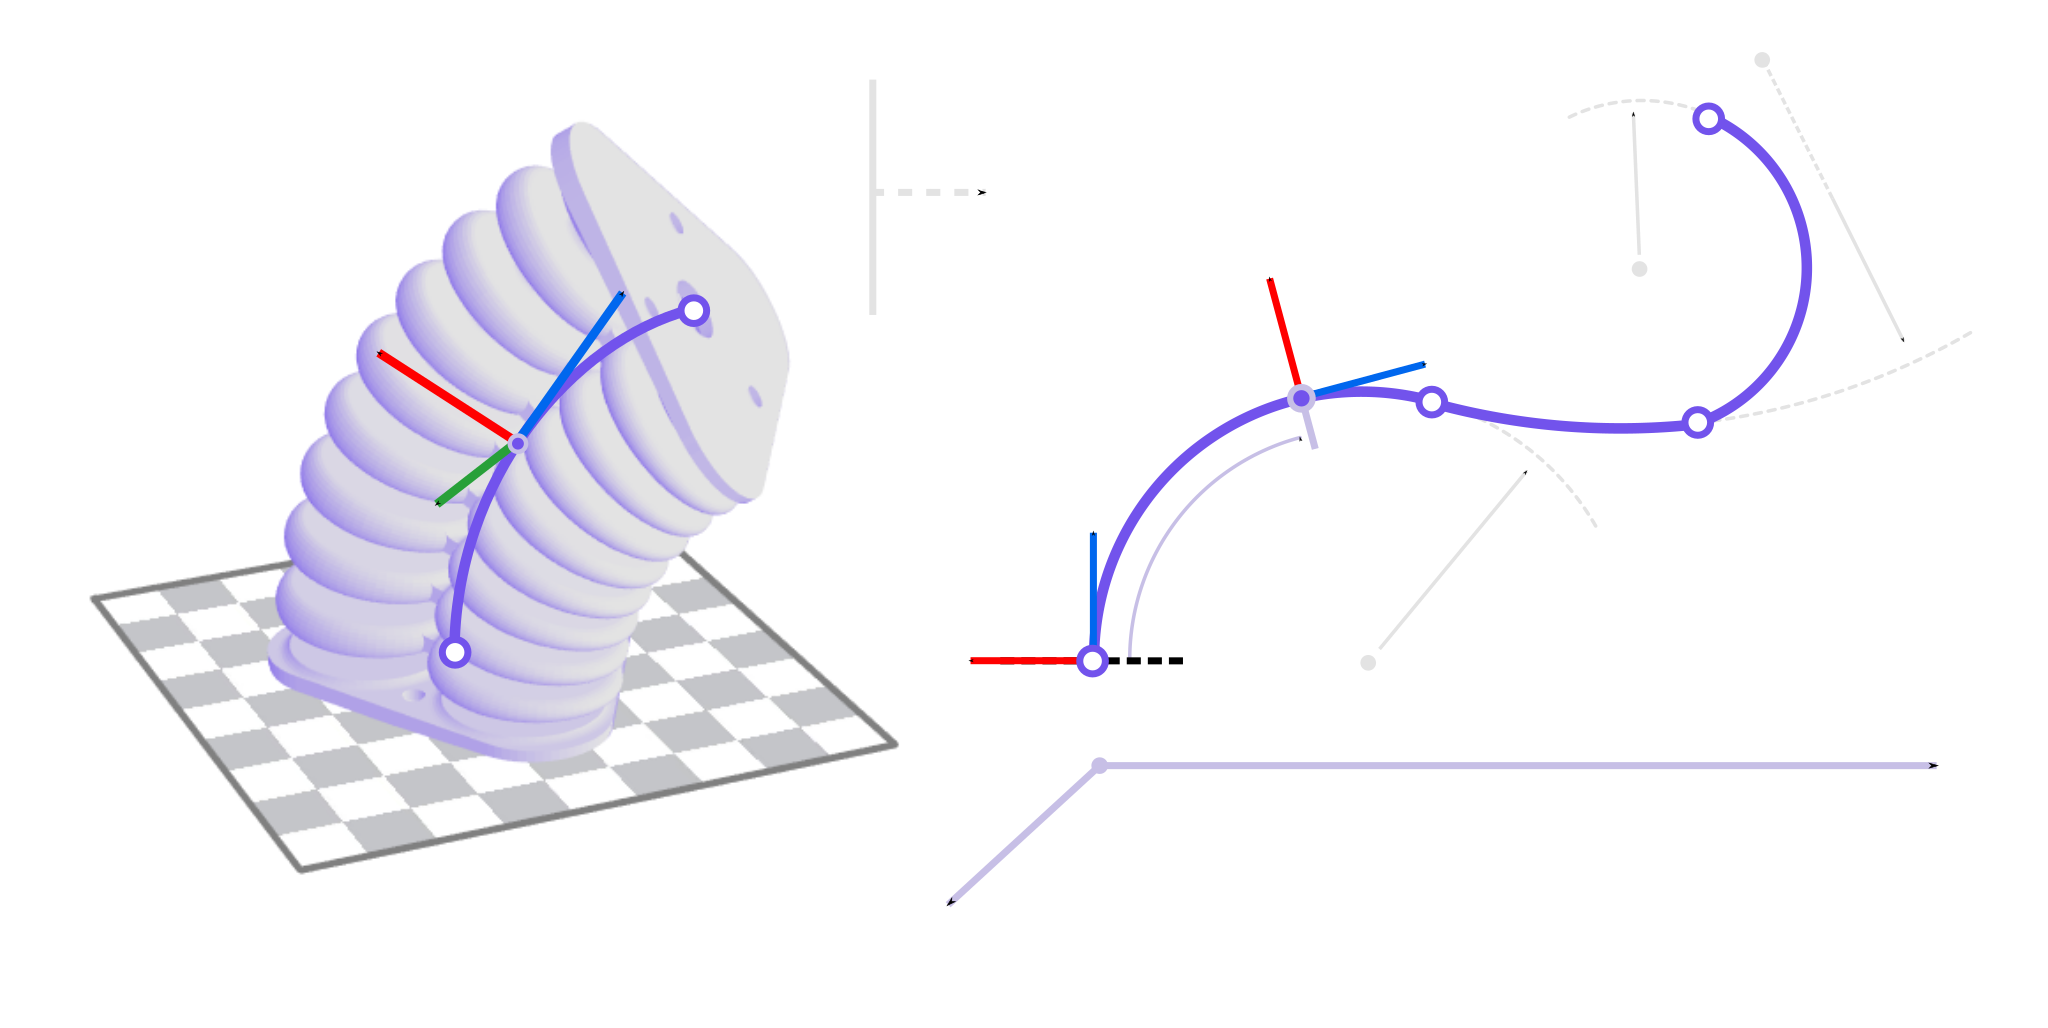
\includegraphics[width = 0.99\textwidth]{fig_C2_schematic.pdf}
  \fi
  \caption{Schematic representation of the Piece-wise Constant Curvature model (PCC) for general soft robotic system, given by a parameterized curve $^0 \gammaB: \Xs \times \Ts \to \R^3$ and orientation matrix $^0 \PhiB: \Xs \times \Ts \to \SO{3}$. The frame $\{\sigma\}$ is rigidly attached to $^0 \gammaB$ such that variation of $\sigma$ give insight into the differential geometry of the curve.}
  \label{fig:C2:configuration}
\end{figure}
%
\begin{dfn}[Piece-wise Constant Curvature]
Despite the inherent flexibility in soft robotics, it is sometimes sufficient to express the kinematics according to the \emph{Piecewise Constant Curvature} (PCC) condition. Mathematically, it implies that the curvature of the continuous body satisfies $\kappa(\sigma_1,\q) = \kappa(\sigma_2,\q)$ for a neighboring region of points $\sigma_1,\sigma_2 \subseteq \Xs$. As a result, this condition allows us to describe the full forward kinematics with a significantly reduced set of generalized coordinates, mitigating kinematic complexity in the model. Numerous works employ PCC models \cite{Falkenhahn2015,Katzschmann2019,Tatlicioglu2007,Marchese2016,Godage2016,DellaSantina2020a}, and depending on the elasticity, the PCC condition has been proven to be consistent for various soft robotic systems.
\end{dfn}
%
{Following this Constant Curvature (CC) description, let us assign a coordinate frame that twists minimally along the backbone -- formally called the \emph{Bishop frame} (see, \cite{Bishop1975}) -- parametrized by the following generalized coordinate vector:}
%
\begin{equation}
\vec{q} := \begin{pmatrix}
\,\varepsilon & \kappa_x & \kappa_y\,
\end{pmatrix}^\top \in \mathcal{Q},
\label{eq:C2:coordinate}
\end{equation}
%
\noindent where $\varepsilon_{-} \le \varepsilon \le \varepsilon_{+}$ is the elongation strain, and $\kappa_x,\,\kappa_y\in\mathbb{R}$ are the curvatures or angular strains in $x$-$z$ and $y$-$z$ plane, respectively; and
$\mathcal{Q} \subset \R^3$ is an admissible space on which $\q$ evolves. Also, we denote the total curvature by $\kappa = \inner{\kappa_x}{\kappa_y}$ together with the curvature angle $\phi = \atantwo(\kappa_y,\kappa_x)$. It is worth mentioning that the joint description above is somewhat related to Renda. et al. (2018, \cite{Renda2018}) who proposed a \emph{Piece-wise Constant Strain} (PCS) parametrization with the exception of including the twist along the tangent.

By exploring the differential geometry of the smooth backbone curve similar to Mochiyama et al. (2003, \cite{Mochiyama2003}), we can write the position vector $\gammaB(\sigma,\q)$ and the orientation matrix $\PhiB(\sigma,\q)$ for each material point $\sigma$ along the smooth backbone as a differential equality of the form:
%
\begin{align}
\renewcommand*{\arraystretch}{2}{}
\frac{\partial \,\!\mat{\Phi}}{\partial \sigma}(\sigma,\q) & = \, \mat{\Phi}(\sigma,\vec{q}) \,\mat{\Gamma}^{\times} (\sigma,\q) \label{eq:C2:change_phi} \\[0.45em]
%
\frac{\partial \, \gammaB}{\partial \sigma}(\sigma,\q) & = \, \mat{\Phi}(\sigma,\vec{q}) \, \vec{U}(\sigma,\q), \label{eq:C2:change_p}
\end{align}
%
where $\vec{\Gamma}^\times \in \SO{3}$ is a skew-symmetric matrix composed of the entries of the vector $\vec{\Gamma} \in \R^3$, and $\vec{U}\in \R^3$ a vector representing the tangent along the extensible backbone. For readers familiar with Lie Groups, the operator $(\,\cdot\,)^\times$ denotes the isomorphism between the Lie algebra $\sog{3}$ and $\R^3$. The vectors $\vec{\Gamma}$ and $\vec{U}$ are vectors that define the differential geometry of the backbone
\cite{Mochiyama2003} which are unique entries that live in the tangent space of the rigid-body transformation group, \ie, $T_{\SE{3}}$. Given the Bishop parametrization as described by \eqref{eq:C2:coordinate} and assuming the Constant-Strain (CC) condition, these geometric entities yield
%
\begin{align}
\vec{\Gamma}(\sigma,t) & \cong \vec{\Gamma}(\sigma,\q(t)) \quad \xRightarrow[]{\textrm{CC condition}}\quad \vec{\Gamma}(\q) = \begin{pmatrix} \;-\kappa_y\;\; \\ \;\kappa_x\;\; \\ \;0\;\;  \end{pmatrix}, \\[0.35em]
%
\vec{U}(\sigma,t) & \cong \vec{U}(\sigma,\q(t)) \!\quad \xRightarrow[]{\textrm{CC condition}} \quad \vec{U}(\q) =  \begin{pmatrix} \;0\;\;  \\  \;0\;\; \\ \varepsilon + 1\ \end{pmatrix},
\end{align}
%
%with $\vec{U}^\circ$ the unit-tangent pointing, and $\vec{\Gamma}^\circ$ the intrinsic curvature/torsion of the curve. For simplicity, lets assume $\vec{U}^\circ = (0,0,1)^\top$ and $\vec{\Gamma}^\circ = \vec{0}_3$.
Now, given an initial configuration of backbone's base, \ie,$\mat{\Phi}(0,\vec{q}) = \vec{\Phi}_0$ and $ \gammaB(0,\q) = \vec{0}_3$, we can now solve for the position and orientation for each material coordinate $\sigma$ along the backbone:
%
\begin{align}
\mat{\Phi}(\sigma,\vec{q}) & = \vec{\Phi}_0\exp_{\SO{3}}(\sigma \vec{\Gamma}^\times(\vec{q})), \label{eq:C2:phi_exact} \\[0.35em]
\gammaB(\sigma,\vec{q}) & = \int_0^\sigma\,^0\mat{\Phi}(\eta,\vec{q})\, \vec{U}(\vec{q}) \; d\eta,
\label{eq:C2:pos_exact}
\end{align}
%
where $\exp_{\SO{3}}: \sog{3} \to \SO{3}$ is the exponential map. Luckily, there exist a compact expression for the exponential mapping related to the orthogonal group of rotation matrices $\SO{3}$ called the \emph{Rodriguez formulas}. Given the rotation angle $\theta(\sigma,\q) := \int_0^\sigma \kappa(s,\q) \; ds = \kappa(\q) \sigma$, we can compactly rewrite the rotation matrix \eqref{eq:C2:phi_exact} in terms of $\cos(\theta)$ and $\sin(\theta)$ using these formulas as follows \cite{Lynch2017}:
%
\begin{equation}
\PhiB(\theta) = \PhiB_0 \left( \mat{I}_3 + \left[ \frac{\sin(\theta)}{\theta} \right]  \GammaB^{\times} + \left[ \frac{1-\cos(\theta)}{\theta^2} \right]  \GammaB^{\times} \GammaB^{\times} \right).
\label{eq:C2:phi_rodr}
\end{equation}
%
We wish to inform the reader that the closed-form solutions \eqref{eq:C2:phi_exact} and \eqref{eq:C2:pos_exact} represent the forward configuration kinematics of the backbone curve. To express the forward velocity kinematic, let
$\etaB(\sigma,\q,\dq) = \left( \vec{\omega}^\top, \vec{v}^\top \right)^\top \in \R^6 \cong \seg{3}$
 be the aggregate of the angular velocity and linear velocity components relative to an inertial frame at $\sigma$, where the space $\seg{3}$ denotes the Lie algebra of $\SE{3}$. The velocity twist is computed by the following integration procedure:
%
\begin{align}
 \etaB(\sigma,\q,\dq) = \Ad_{\mat{g}(\sigma,\cdot)}\inv \int_0^\sigma \Ad_{\mat{g}(s,\cdot)}\, \JB^\star\! \dq\;ds
 \,=:\, \JB(\q,\sigma) \dq, \label{eq:C2:vel_cont}
\end{align}
%
where $\Ad_g: \SE{3} \to \mathbb{R}^{6\times 6}$ denotes the adjoint transformation matrix regarding the rigid body transformation $\gB \in \SE{3}$ that maps local velocities (i.e., twist) to a frame located at $\sigma$, and $\JB^\star:\Q \to T_{\q}\Q$ the joint-axis matrix that relates the DOFs to the geometric deformations. Let it be clear that the joint-axis matrix is naturally constant for a soft segment modeled with the Constant-Strain (CS) assumption. We will later relax this assumption in Chapter 4. Nevertheless here, the joint-axis matrix for an extensible and bendable CS segment parametrized by the Bishop parameters is given by
%
\begin{align}
\renewcommand*{\arraystretch}{1}{}
\JB^\star := \begin{pmatrix}\dfrac{\p \GammaB}{\p \q}^\top & \dfrac{\p \UB}{\p \q}^\top \end{pmatrix}^\top  = \begin{pmatrix}
\,0 & 0 & 0 & 0 & 0 & 1 \, \\
\,0 & 1 & 0 & 0 & 0 & 0 \,  \\
\,-1 & 0 & 0 & 0 & 0 & 0 \,  \\
\end{pmatrix}^\top. \label{eq:C2:joint-axis-matrix}
\end{align}
%
Although we based the forward kinematics on the work of Mochiyama et al.\cite{Mochiyama2003}, the derived expression for the velocity twist in \eqref{eq:C2:vel_cont} is analogous to the work of Renda et al. (2018, 2020; \cite{Renda2018,Renda2020}), and Boyer et al. (2010, 2021; \cite{Boyer2010,Boyer2021}). Please also note that
\eqref{eq:C2:vel_cont} gives rise to the geometric manipulator Jacobian $\JB(\sigma,\q)$ that defines the mapping from joint velocities to the velocity twist for a point $\sigma$ on the elastic body.

In continuation, let us also introduce the acceleration twist \cite{Boyer2021,Mochiyama2003,Renda2018} -- obtained through time differentiation of \eqref{eq:C2:vel_cont}:
%
\begin{align}
\dot{\etaB}(\sigma,\q,\dq,\ddq) & = \JB \ddot{\q} + \Ad_{\gB(\cdot,\sigma)} \inv \int_0^\sigma \Ad_{\gB(s,\cdot)}
\ad_{\etaB(s,\cdot,\cdot)} \, \JB^\star\! \dq \;ds \notag \\
& :=  \JB(\sigma,\q)\ddot{\q} + \dmat{J}(\sigma,\q,\dot{\q}) \dot{\q},
\label{eq:C2:acceleration}
\end{align}
%
where $\ad_{\etaB}: \R^{6} \to \R^{6\times 6}$ denotes the adjoint transformation regarding the velocity twist $\vec{\etaB}^\wedge \in \seg{3}$. The reader is referred to Appendix \ref{app:C2:adjoint} for more detailed expressions on the adjoint transformations.
%
\begin{rmk}[Numerical instability near zero-curvature] In many of the PCC modeling literate there are mentions of a singularity point when the soft robot $\kappa \to 0$, stating that the linear velocities $\vec{v} := \floor{\etaB}_3$ are not well-defined and thus may be unbounded. However, this is perhaps a common misconception in literate is mainly caused by numerical instability. To illustrate, consider the inextensible planar case: $\varepsilon = \kappa_y = 0$ and $\kappa = \kappa_x$. Hence, by solving the forward kinematics for the position vector $\gammaB(\sigma,\kappa)$, and taking the approaching zero from the positive domain $\kappa^{+} \to 0$, we see that
%
\begin{align}
\lim_{\kappa \to \,0^{+}}\gammaB(\sigma,\kappa) & = \begin{pmatrix} \dfrac{1-\cos(\sigma \kappa)}{\kappa}\,, & 0\,, & \dfrac{\sin(\sigma \kappa)}{\kappa} \end{pmatrix}^\top = \begin{pmatrix} 0 & 0 & \sigma \end{pmatrix}^\top,
\end{align}
%
which is clearly well-defined. Since the position vector $\gammaB$ is continuously differentiable when approaching the origin from both sides $\kappa \to 0^+$ and $\kappa \to 0^{-}$, it follows that $\dot{\gammaB}$ must be bounded for all $\kappa \in \Q$. We can simply check this by investigating the behavior of the linear-velocity portion of the geometric Jacobian near zero-curvature, which yields
%
\begin{align}
\lim_{\kappa \to \,0^+} \floor{\JB}_3(\sigma,\kappa) & = \begin{pmatrix} \tfrac{\sigma \kappa \sin(\sigma \kappa) + 1 - \cos(\sigma \kappa)}{\kappa^2}\,, & 0\,, & \tfrac{\sigma \kappa \cos(\sigma \kappa) - \sin(\sigma \kappa) }{\kappa^2} \end{pmatrix}^\top \notag \\[0.35em] & = \begin{pmatrix} \sigma^2 & 0 & 0 \end{pmatrix}^\top.
\end{align}
%
Again, the expression is well-defined. Consequently, the magnitude of the linear velocity of the end-effector reads simply $\lVert \dot{\gammaB}(L,\dot{\kappa}) \rVert = L^2\dot{\kappa} = L \omega_1$ with $\omega_1$ the angular velocity at the tip. This naturally poses an ambiguity on the origin of this kinematic singularity. The problem is, however, of numerical origin when considering the zero-division. To make matters worse, deriving analytical expressions for accelerations will contain similar expressions that are hard to stabilize numerically. To resolve this issue, we opt for a numerical approximation of the forward kinematics -- namely, we employ an explicit forward integration scheme (\ie, trapezoidal integration) to solve \eqref{eq:C2:change_phi} and \eqref{eq:C2:change_p}.
\end{rmk}

\newpage
\begin{example}[Kinematic behavior of PCC segment]
As an illustrative example, we provide simulation of the forward kinematics for a single PCC segment given predefined trajectory on the geometric join variables $\q(t) \equiv \q_d(t)$, $\dot{\q}(t) \equiv \dot{\q}_d(t)$ and $\ddot{\q}(t) \equiv \ddot{\q}_r(t)$. Let us consider the following reference trajectory for the 3-DOF soft manipulator:
%
\begin{align*}
\q_d(t) &  =  \erf(t) \cdot \begin{pmatrix} \varepsilon_0 \sin(\omega t) & \kappa_0 \cos(\omega t) & \kappa_0 \sin(\tfrac{3}{2}\omega t - \tfrac{\pi}{4}) \end{pmatrix}^\top,
\end{align*}
%
where $\textrm{erf}(t) := \frac{2}{\pi}\int_0^\tau \exp(-\tau^2) \; d\tau$ is referred to as the error function. Note that these are smooth functions such that reference velocity $\dq_d$ and reference acceleration $\ddq_d$ exist and are bounded. The reference signals for the geometric strain of the soft robot are shown in Figure \ref{fig:C2:EX1:strain_ref}. Let it be clear that the reference $\q_d$ has been carefully selected to ensure it passes the line $\kappa_x = \kappa_y = 0$ on the configuration space
$\mathcal{Q}$, \ie, the numerical instability point for near-zero curvature..

Then, by inject the reference into the kinematic relations described by the expressions \eqref{eq:C2:change_phi}, \eqref{eq:C2:change_p}, \eqref{eq:C2:vel_cont}, and \eqref{eq:C2:acceleration}, we obtain a (close) approximation of forward kinematics as shown in Figure
\ref{fig:C2:EX1:strain_ref_FK}. Furthermore, we provided a 3D-rendering of the soft robot subjected to the reference $\q_d$ in Figure \ref{fig:C2:EX1:strain_ref_3D}. Now, two key observations can be made. First, although a simple harmonic trajectory is used, the resulting trajectory of the end-effector as shown in Figure \ref{fig:C2:EX1:strain_ref_FK} is rather complex. This perhaps stresses the importance of inverse kinematic solver that can be used for task-space control. Second, although we pass the point of numerical instability for
$\kappa \to 0$, we see that the velocity solutions are smooth and bounded at these instances. This result shows our approach does not suffer from the near-zero curvature instabilities that are notoriously mentioned in \cite{Falkenhahn2015,DellaSantina2020}, yet at the cost of providing an analytical expression.

\begin{figure}[!b]
  %\vspace{-0mm}
  %\centering
  \ifx\printFigures1\undefined
  \else
  % This file was created by matlab2tikz.
%
\definecolor{mycolor1}{rgb}{0.00000,0.34510,0.65882}%
\definecolor{mycolor2}{rgb}{0.79216,0.11765,0.17255}%
\definecolor{mycolor3}{rgb}{0.20392,0.65490,0.24706}%
%
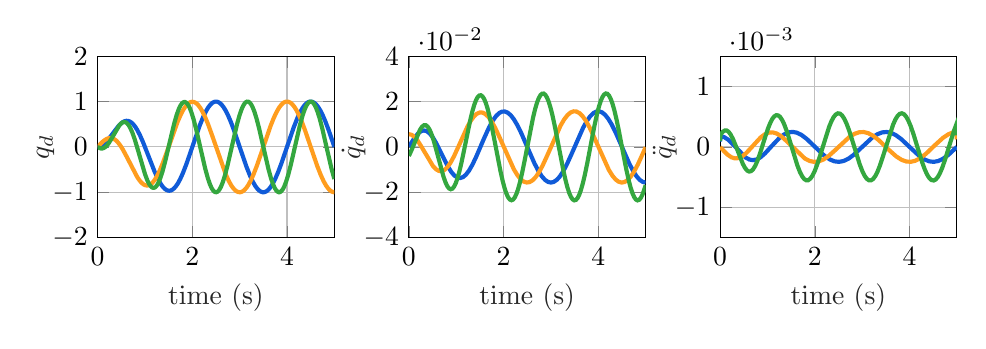
\begin{tikzpicture}

\begin{axis}[%
width=0.248\textwidth,
height=0.19\textwidth,
at={(0\textwidth,0\textwidth)},
scale only axis,
xmin=0,
xmax=5,
xlabel style={font=\color{white!15!black}},
xlabel={time (s)},
ymin=-2,
ymax=2,
ylabel style={font=\color{white!15!black}},
ylabel={$q_d$},
axis background/.style={fill=white},
xmajorgrids,
ymajorgrids,
ylabel style={yshift=-7.5pt}
]
\addplot [color=mycolor1, line width=1.5pt, forget plot]
  table[row sep=crcr]{%
0	0\\
0.035035035035035	0.00434065382436177\\
0.075075075075075	0.0197581919620422\\
0.115115115115115	0.0457558239801097\\
0.16016016016016	0.0864034559537759\\
0.215215215215215	0.149650792611576\\
0.29029029029029	0.251909193908196\\
0.435435435435435	0.452501851145034\\
0.49049049049049	0.511874966215594\\
0.535535535535535	0.547735702552471\\
0.575575575575575	0.567954316778994\\
0.61061061061061	0.575566933229249\\
0.645645645645645	0.573088771427073\\
0.68068068068068	0.560095653946306\\
0.715715715715715	0.536392535810649\\
0.755755755755755	0.496246230155413\\
0.795795795795796	0.442585433729294\\
0.840840840840841	0.367062318903137\\
0.895895895895896	0.255345156916537\\
0.960960960960961	0.101033017828754\\
1.05605605605606	-0.15149073785141\\
1.20620620620621	-0.550319348528045\\
1.27627627627628	-0.708764889034357\\
1.33133133133133	-0.811325353645943\\
1.37637637637638	-0.877772299605288\\
1.41641641641642	-0.922105295564261\\
1.45145145145145	-0.948751619733451\\
1.48648648648649	-0.963596043213059\\
1.51651651651652	-0.966718567647844\\
1.54654654654655	-0.960902245684151\\
1.57657657657658	-0.946171019746461\\
1.61161161161161	-0.91787491799227\\
1.65165165165165	-0.871308378489516\\
1.6966966966967	-0.801691383211872\\
1.74674674674675	-0.704652917692613\\
1.8018018018018	-0.576880303587744\\
1.87187187187187	-0.388564855615353\\
1.96696696696697	-0.103030019623617\\
2.15715715715716	0.472826180715402\\
2.22722722722723	0.653682856913231\\
2.28728728728729	0.783947303234589\\
2.33733733733734	0.871419229432251\\
2.38238238238238	0.931802645757189\\
2.42242242242242	0.969852863853533\\
2.45745745745746	0.990576346388929\\
2.48748748748749	0.99879275130267\\
2.51751751751752	0.998116211770342\\
2.54754754754755	0.988552949224476\\
2.58258258258258	0.966282396359661\\
2.61761761761762	0.932306066362887\\
2.65765765765766	0.87967759968175\\
2.7027027027027	0.803890788095862\\
2.75275275275275	0.700895927035849\\
2.81281281281281	0.554714287228555\\
2.88788788788789	0.344958268771602\\
3.003003003003	-0.00943386773232557\\
3.14314314314314	-0.43468926190012\\
3.21821821821822	-0.633097599682777\\
3.27827827827828	-0.767051472600784\\
3.32832832832833	-0.858054673447568\\
3.37337337337337	-0.921910196927753\\
3.41341341341341	-0.963228857786627\\
3.44844844844845	-0.986913031185399\\
3.48348348348348	-0.998653274574725\\
3.51351351351351	-0.999098293329462\\
3.54354354354354	-0.990657463060607\\
3.57857857857858	-0.96968362697153\\
3.61361361361361	-0.936974398085302\\
3.65365365365365	-0.885736697748763\\
3.6986986986987	-0.811413049476992\\
3.74874874874875	-0.709880810775015\\
3.80880880880881	-0.565174526154613\\
3.88388388388388	-0.356752674288018\\
3.99399399399399	-0.0188673044788441\\
4.14414414414414	0.437523008440333\\
4.21921921921922	0.635532084307429\\
4.27927927927928	0.769068005472834\\
4.32932932932933	0.859667579389312\\
4.37437437437437	0.923125598625732\\
4.41441441441441	0.964070346402118\\
4.44944944944945	0.987416293148271\\
4.48448448448448	0.998812274000765\\
4.51451451451451	0.998960559587034\\
4.54454454454454	0.990224253362287\\
4.57957957957958	0.968910783145196\\
4.61461461461461	0.935871305490616\\
4.65465465465465	0.884272782967919\\
4.6996996996997	0.809571163316425\\
4.74974974974975	0.707662478873392\\
4.80980980980981	0.562577458212637\\
4.88488488488488	0.353813119124604\\
5	8.88178419700125e-16\\
};
\addplot [color=mycolor2, line width=1.5pt, forget plot]
  table[row sep=crcr]{%
0	0\\
0.105105105105105	0.111779765028618\\
0.16016016016016	0.156980153648786\\
0.205205205205205	0.182511422079791\\
0.245245245245245	0.194668024428809\\
0.28028028028028	0.196227360736436\\
0.315315315315315	0.188769317384463\\
0.35035035035035	0.172022106528288\\
0.39039039039039	0.141487076700804\\
0.43043043043043	0.0991512285511922\\
0.475475475475475	0.0383838014112809\\
0.53053053053053	-0.0523767761630261\\
0.6006006006006	-0.18783198174113\\
0.840840840840841	-0.67188191620076\\
0.895895895895896	-0.752708585608064\\
0.940940940940941	-0.802692146771466\\
0.980980980980981	-0.833165316743078\\
1.01601601601602	-0.848168474733675\\
1.04604604604605	-0.851956160757179\\
1.07607607607608	-0.847156376186706\\
1.10610610610611	-0.833681829324347\\
1.14114114114114	-0.807033343602345\\
1.17617617617618	-0.768832354621136\\
1.21621621621622	-0.711564770634355\\
1.26126126126126	-0.63088812208567\\
1.31631631631632	-0.511373504538406\\
1.38138138138138	-0.345607907267669\\
1.46646646646647	-0.101148746562225\\
1.68668668668669	0.544000207265759\\
1.75175175175175	0.701576721741857\\
1.80680680680681	0.812683401978535\\
1.85685685685686	0.892797948975148\\
1.8968968968969	0.941073870130205\\
1.93193193193193	0.971074104183863\\
1.96696696696697	0.989241847338064\\
1.996996996997	0.995215537037103\\
2.02702702702703	0.992264006504053\\
2.05705705705706	0.980411255152744\\
2.09209209209209	0.95547795269928\\
2.12712712712713	0.918880529317171\\
2.16716716716717	0.863353759912902\\
2.21221221221221	0.7844957377737\\
2.26726726726727	0.666829747058395\\
2.33233233233233	0.502232140204002\\
2.41241241241241	0.271529840930044\\
2.7027027027027	-0.594554525970798\\
2.76776776776777	-0.745387426665372\\
2.82282282282282	-0.848990849411984\\
2.86786786786787	-0.915028120952007\\
2.90790790790791	-0.958401759441889\\
2.94294294294294	-0.983946634072939\\
2.97797797797798	-0.997582418387913\\
3.00800800800801	-0.999662561645784\\
3.03803803803804	-0.992851132434541\\
3.06806806806807	-0.977208771789291\\
3.1031031031031	-0.947988039568602\\
3.14314314314314	-0.900570748735437\\
3.18818818818819	-0.830261109785634\\
3.23823823823824	-0.732742817227718\\
3.29329329329329	-0.604697368948116\\
3.36336336336336	-0.41619419138787\\
3.45845845845846	-0.1301363223696\\
3.65365365365365	0.464187490802019\\
3.72372372372372	0.646393867785127\\
3.78378378378378	0.778035686293484\\
3.83383383383383	0.866810466126059\\
3.87887887887888	0.928474109611159\\
3.91891891891892	0.967732918025878\\
3.95395395395395	0.989555253702245\\
3.98398398398398	0.998734409694203\\
4.01401401401401	0.999030984234652\\
4.04404404404404	0.990442339782819\\
4.07907907907908	0.969298597922351\\
4.11411411411411	0.9364241544223\\
4.15415415415415	0.88500593597636\\
4.1991991991992	0.810493174479892\\
4.24924924924925	0.708772560434584\\
4.30930930930931	0.563876708920316\\
4.38438438438438	0.35528334276137\\
4.49449449449449	0.0172951932970005\\
4.63963963963964	-0.424754659261413\\
4.71471471471471	-0.624542944420901\\
4.77477477477477	-0.759946247977657\\
4.82482482482482	-0.852352489109542\\
4.86986986986987	-0.917592188634139\\
4.90990990990991	-0.96021468537402\\
4.94494494494494	-0.985079574464464\\
4.97997997997998	-0.99802277725853\\
5	-0.999999999998463\\
};
\addplot [color=mycolor3, line width=1.5pt, forget plot]
  table[row sep=crcr]{%
0	-0\\
0.04004004004004	-0.0253745100040801\\
0.07007007007007	-0.0347038050172159\\
0.1001001001001	-0.0347370008429007\\
0.13013013013013	-0.0250154145793022\\
0.16016016016016	-0.0054932552761473\\
0.195195195195195	0.0291506297466535\\
0.235235235235235	0.0827538361897568\\
0.285285285285285	0.16619460726963\\
0.46046046046046	0.476679866800188\\
0.5005005005005	0.520938149913881\\
0.53053053053053	0.541265433708041\\
0.555555555555555	0.548589477479468\\
0.58058058058058	0.546477201874926\\
0.605605605605605	0.534475742154076\\
0.63063063063063	0.512334606754345\\
0.66066066066066	0.472339342305941\\
0.695695695695695	0.407638563999009\\
0.735735735735735	0.311549516304309\\
0.785785785785786	0.162988678062016\\
0.850850850850851	-0.0635843329845418\\
1.001001001001	-0.598978538317431\\
1.05105105105105	-0.737906954073797\\
1.09109109109109	-0.822134211231833\\
1.12112112112112	-0.866793223366643\\
1.14614614614615	-0.890778796998402\\
1.17117117117117	-0.902132835176695\\
1.19119119119119	-0.901877449005232\\
1.21121121121121	-0.893224311557399\\
1.23623623623624	-0.870611388147704\\
1.26126126126126	-0.835084370833918\\
1.29129129129129	-0.775989311963286\\
1.32632632632633	-0.685754032567514\\
1.37137137137137	-0.539824281580024\\
1.42642642642643	-0.324964646431106\\
1.51151151151151	0.0524552962322513\\
1.61661661661662	0.51068147425186\\
1.67167167167167	0.710508039285358\\
1.71671671671672	0.839809432175977\\
1.75175175175175	0.914737029146651\\
1.78178178178178	0.959240382698092\\
1.80680680680681	0.981667705873682\\
1.82682682682683	0.989754892345688\\
1.84684684684685	0.988985560607153\\
1.86686686686687	0.979356598439477\\
1.89189189189189	0.954987957816951\\
1.91691691691692	0.917231880765766\\
1.94694694694695	0.854996252662267\\
1.98198198198198	0.760654843428203\\
2.02702702702703	0.609027332372115\\
2.08208208208208	0.386868838337833\\
2.16716716716717	-0.00235341420373558\\
2.27227227227227	-0.476740013733818\\
2.32732732732733	-0.686128439736638\\
2.37237237237237	-0.823872463922093\\
2.40740740740741	-0.905707232186816\\
2.43743743743744	-0.956312435519591\\
2.46246246246246	-0.983906356917698\\
2.48748748748749	-0.997827816311879\\
2.50750750750751	-0.99898359601381\\
2.52752752752753	-0.991250100548469\\
2.55255255255255	-0.969194596213682\\
2.57757757757758	-0.933668618821868\\
2.60760760760761	-0.873964134919092\\
2.64264264264264	-0.782315745941585\\
2.68768768768769	-0.633618002235095\\
2.74274274274274	-0.414005821608413\\
2.82282282282282	-0.0495061227704499\\
2.94294294294294	0.493844251052776\\
2.997997997998	0.700388748460756\\
3.04304304304304	0.835041499681637\\
3.07807807807808	0.914107856575382\\
3.10810810810811	0.962155969131873\\
3.13313313313313	0.98753105117545\\
3.15815815815816	0.99918833543435\\
3.17817817817818	0.998522048373447\\
3.1981981981982	0.988974942633285\\
3.22322322322322	0.964689233243766\\
3.24824824824825	0.927003009137534\\
3.27827827827828	0.864840650298925\\
3.31331331331331	0.770571225684974\\
3.35835835835836	0.619000071754701\\
3.41341341341341	0.396800981518273\\
3.4984984984985	0.00707559477390074\\
3.60860860860861	-0.489752472097759\\
3.66366366366366	-0.697029667042679\\
3.70870870870871	-0.832450937165657\\
3.74374374374374	-0.912197337060987\\
3.77377377377377	-0.960870579525157\\
3.7987987987988	-0.986786943557313\\
3.82382382382382	-0.998996023815813\\
3.84384384384384	-0.998773604988724\\
3.86386386386386	-0.989668255700024\\
3.88888888888889	-0.965925789545627\\
3.91391391391391	-0.928765818557316\\
3.94394394394394	-0.86720224931259\\
3.97897897897898	-0.77357123059458\\
4.02402402402402	-0.622699193733973\\
4.07907907907908	-0.401126949383538\\
4.16416416416416	-0.0117924918369763\\
4.27427427427427	0.485634538435109\\
4.32932932932933	0.693639713954403\\
4.37437437437437	0.82982807333996\\
4.40940940940941	0.910254465460059\\
4.43943943943944	0.959553358610013\\
4.46446446446446	0.986011765731368\\
4.48948948948949	0.998773659190625\\
4.50950950950951	0.998996087409785\\
4.52952952952953	0.990333607846368\\
4.55455455455455	0.967135952108439\\
4.57957957957958	0.930503983273733\\
4.60960960960961	0.869541525097858\\
4.64464464464464	0.776551901449321\\
4.68968968968969	0.626383213058514\\
4.74474474474474	0.405443448982906\\
4.82982982982983	0.0165091212806967\\
4.93993993993994	-0.481505636914043\\
4.99499499499499	-0.690234174264289\\
5	-0.707106781185458\\
};
\end{axis}

\begin{axis}[%
width=0.248\textwidth,
height=0.19\textwidth,
at={(0.326\textwidth,0\textwidth)},
scale only axis,
xmin=0,
xmax=5,
xlabel style={font=\color{white!15!black}},
xlabel={time (s)},
ymin=-0.04,
ymax=0.04,
ylabel style={font=\color{white!15!black}},
ylabel={$\dot{q}_d$},
axis background/.style={fill=white},
xmajorgrids,
ymajorgrids,
ylabel style={yshift=-7.5pt}
]
\addplot [color=mycolor1, line width=1.5pt, forget plot]
  table[row sep=crcr]{%
0	8.87958036743797e-05\\
0.02002002002002	0.000709205286566927\\
0.13013013013013	0.00431354598848444\\
0.2002002002002	0.00602568516306956\\
0.26026026026026	0.00693784257997976\\
0.32032032032032	0.00724490259747501\\
0.38038038038038	0.00690746540709775\\
0.44044044044044	0.00593471651671429\\
0.505505505505505	0.00422996742472659\\
0.575575575575575	0.00177973755126715\\
0.675675675675675	-0.00240049325539715\\
0.825825825825826	-0.00868090425285217\\
0.900900900900901	-0.0111658143824966\\
0.965965965965966	-0.0127084883031694\\
1.02602602602603	-0.0135312743668141\\
1.08608608608609	-0.0137280496105907\\
1.14614614614615	-0.0132868669616926\\
1.20620620620621	-0.0122291022584786\\
1.27127127127127	-0.0104477195110757\\
1.34134134134134	-0.0079022607533874\\
1.42642642642643	-0.00416316463676836\\
1.58658658658659	0.00368059325814496\\
1.69169169169169	0.00849151878580301\\
1.77177177177177	0.0115460906314997\\
1.84184184184184	0.0136041791124057\\
1.90690690690691	0.0149070651732561\\
1.96696696696697	0.0155416553906065\\
2.02702702702703	0.0156092580414757\\
2.08708708708709	0.0151099515853312\\
2.15215215215215	0.0139534009546507\\
2.21721721721722	0.01220713173322\\
2.29229229229229	0.00955913862891311\\
2.37737737737738	0.0059220893298475\\
2.5025025025025	-0.000112795085106754\\
2.65265265265265	-0.00724892771459817\\
2.73773773773774	-0.0106779731168718\\
2.80780780780781	-0.012940911941616\\
2.87287287287287	-0.0144843869759752\\
2.93793793793794	-0.0154244334183069\\
2.997997997998	-0.0157223717405444\\
3.05805805805806	-0.0154620801493941\\
3.12312312312312	-0.0145613972166379\\
3.18818818818819	-0.0130543490417994\\
3.25825825825826	-0.0108257718717653\\
3.33833833833834	-0.00764650755058938\\
3.43843843843844	-0.00302197280326677\\
3.67867867867868	0.00836963830915671\\
3.75875875875876	0.0114195404408468\\
3.82882882882883	0.0135039386224447\\
3.89389389389389	0.0148575485231452\\
3.95895895895896	0.0155925293693473\\
4.01901901901902	0.01569498110561\\
4.07907907907908	0.0152403197954696\\
4.14414414414414	0.0141382701809354\\
4.20920920920921	0.0124475408105065\\
4.27927927927928	0.0100496470917113\\
4.36436436436436	0.00649885919009208\\
4.47947947947948	0.00101291704575601\\
4.65465465465465	-0.00734219873027886\\
4.73973973973974	-0.0107537859157611\\
4.80980980980981	-0.0129989373491224\\
4.87487487487487	-0.0145238276366495\\
4.93993993993994	-0.0154439846312249\\
5	-0.0157230390570149\\
};
\addplot [color=mycolor2, line width=1.5pt, forget plot]
  table[row sep=crcr]{%
0	0.00564679810898916\\
0.06006006006006	0.00532698853810398\\
0.12012012012012	0.00439279220918198\\
0.185185185185185	0.00277385963725596\\
0.265265265265265	0.000135489686829082\\
0.51051051051051	-0.00846723701053786\\
0.575575575575575	-0.00988340148525158\\
0.635635635635635	-0.0105965516072484\\
0.695695695695695	-0.0106745781731705\\
0.755755755755755	-0.0100982489775987\\
0.815815815815816	-0.00889075730022348\\
0.880880880880881	-0.00694328214617457\\
0.950950950950951	-0.00424090998455195\\
1.04604604604605	8.04961082803146e-05\\
1.23623623623624	0.0088695371597316\\
1.31131131131131	0.0116449451465765\\
1.37637637637638	0.0134795293660801\\
1.43643643643644	0.0146177117690955\\
1.4964964964965	0.0151759125248292\\
1.55655655655656	0.0151350477011531\\
1.61661661661662	0.014501321548952\\
1.68168168168168	0.0131809237407268\\
1.74674674674675	0.0112662147885771\\
1.82182182182182	0.00843852080878538\\
1.91191191191191	0.00440679951085077\\
2.21721721721722	-0.00986682322024279\\
2.29229229229229	-0.0124599594878632\\
2.36236236236236	-0.0142550761271227\\
2.42742742742743	-0.0153034838841499\\
2.48748748748749	-0.015703599140477\\
2.54754754754755	-0.0155443311943841\\
2.61261261261261	-0.0147481695643945\\
2.67767767767768	-0.0133367782902223\\
2.74774774774775	-0.0111971986946333\\
2.82282282282282	-0.00830788352575418\\
2.91791791791792	-0.00401063830401949\\
3.2032032032032	0.00936909186312107\\
3.27827827827828	0.0120603023051942\\
3.34834834834835	0.0139720380102135\\
3.41341341341341	0.0151448717266796\\
3.47847847847848	0.0156870991330482\\
3.53853853853854	0.0156079352179992\\
3.6036036036036	0.0148975351922962\\
3.66866866866867	0.0135668386233387\\
3.73873873873874	0.0115041615729501\\
3.81381381381381	0.00868122055632714\\
3.9039039039039	0.00467492977406625\\
4.22422422422422	-0.0101821280708343\\
4.2992992992993	-0.012699830891715\\
4.36436436436436	-0.0143170802219998\\
4.42942942942943	-0.015338204655519\\
4.49449449449449	-0.0157206873108446\\
4.55455455455455	-0.0154926801893511\\
4.61961961961962	-0.0146258182674659\\
4.68468468468468	-0.0131499764352121\\
4.75475475475475	-0.010950560202887\\
4.83483483483483	-0.00779720158670827\\
4.93493493493493	-0.00319157963644301\\
5	-0.000123614618962264\\
};
\addplot [color=mycolor3, line width=1.5pt, forget plot]
  table[row sep=crcr]{%
0	-0.00389809489151549\\
0.015015015015015	-0.00339743312423035\\
0.07007007007007	-0.000798049903772302\\
0.235235235235235	0.0075242798095152\\
0.28028028028028	0.00891341777412347\\
0.32032032032032	0.00954886517354314\\
0.36036036036036	0.00954325489899865\\
0.4004004004004	0.00886314945613709\\
0.44044044044044	0.00751665139384627\\
0.48048048048048	0.00555306089437746\\
0.525525525525525	0.00271691090566417\\
0.58058058058058	-0.00140005508322449\\
0.73073073073073	-0.013047466318822\\
0.775775775775776	-0.015698623308781\\
0.815815815815816	-0.0174204385094043\\
0.850850850850851	-0.018349425338215\\
0.885885885885886	-0.0186874682652869\\
0.920920920920921	-0.0184077208485345\\
0.955955955955956	-0.0175061165448778\\
0.990990990990991	-0.0160013355837796\\
1.02602602602603	-0.0139339061890249\\
1.06606606606607	-0.0109608486185069\\
1.11111111111111	-0.00698189751919642\\
1.17117117117117	-0.000980351284410652\\
1.2962962962963	0.0117619630177312\\
1.34134134134134	0.0156578685080238\\
1.38138138138138	0.0185348794184224\\
1.41641641641642	0.0205023889787048\\
1.45145145145145	0.0218918110674409\\
1.48648648648649	0.0226596686069893\\
1.52152152152152	0.0227814208285331\\
1.55655655655656	0.0222519519447575\\
1.59159159159159	0.0210854742708797\\
1.62662662662663	0.0193148692864513\\
1.66166166166166	0.0169905040707912\\
1.7017017017017	0.01374157480143\\
1.74674674674675	0.00947671453637522\\
1.80680680680681	0.00312319721480137\\
1.93693693693694	-0.0108766793959374\\
1.98198198198198	-0.0150397082531191\\
2.02202202202202	-0.0181763491351035\\
2.06206206206206	-0.0206640010925963\\
2.0970970970971	-0.0222375006152946\\
2.13213213213213	-0.0232022701913621\\
2.16716716716717	-0.0235320248963236\\
2.2022022022022	-0.0232179498720821\\
2.23723723723724	-0.0222688850183692\\
2.27227227227227	-0.0207110348795023\\
2.30730730730731	-0.0185872130621734\\
2.34734734734735	-0.0155422967374443\\
2.39239239239239	-0.0114608139600945\\
2.44744744744745	-0.00579145047336116\\
2.62262262262262	0.0128741520625955\\
2.66766766766767	0.0167484861142819\\
2.70770770770771	0.0195655424407741\\
2.74274274274274	0.0214633257479662\\
2.77777777777778	0.0227771606090883\\
2.81281281281281	0.0234713332423633\\
2.84784784784785	0.0235269892600414\\
2.88288288288288	0.0229426428669539\\
2.91791791791792	0.0217342145445576\\
2.95295295295295	0.0199345961159061\\
2.99299299299299	0.0172174864691881\\
3.03303303303303	0.0138891400020897\\
3.07807807807808	0.00956198015215293\\
3.13813813813814	0.00316121176298179\\
3.26326326326326	-0.0103680819172496\\
3.30830830830831	-0.0145980008421667\\
3.34834834834835	-0.0178130752410732\\
3.38838838838839	-0.0203958438019916\\
3.42342342342342	-0.0220643905498283\\
3.45845845845846	-0.0231328750670352\\
3.49349349349349	-0.0235722399853806\\
3.52852852852853	-0.0233705372810213\\
3.56356356356356	-0.0225332531602396\\
3.5985985985986	-0.0210831588311615\\
3.63363363363363	-0.0190596912137808\\
3.67367367367367	-0.0161163193506209\\
3.71871871871872	-0.0121272464772959\\
3.76876876876877	-0.00706512219780375\\
3.85385385385385	0.00227697060687326\\
3.92392392392392	0.00976466521871266\\
3.97397397397397	0.0145105874986564\\
4.01401401401401	0.0177400615962862\\
4.05405405405405	0.0203398300274422\\
4.08908908908909	0.0220249114397006\\
4.12412412412412	0.0231110093381206\\
4.15915915915916	0.0235685865111357\\
4.19419419419419	0.0233851988235765\\
4.22922922922923	0.0225658336438439\\
4.26426426426426	0.0211327742088825\\
4.2992992992993	0.0191249936155176\\
4.33933933933934	0.0161973536236735\\
4.38438438438438	0.0122225178974782\\
4.43443443443443	0.00717117600018735\\
4.51951951951952	-0.00216622237303721\\
4.59459459459459	-0.0101679498965721\\
4.64464464464464	-0.0148587632807544\\
4.68468468468468	-0.0180300857626401\\
4.72472472472472	-0.0205614078968743\\
4.75975975975976	-0.0221800565341406\\
4.79479479479479	-0.0231955024176012\\
4.82982982982983	-0.0235801297586606\\
4.86486486486486	-0.0233234783373355\\
4.8998998998999	-0.0224325279755435\\
4.93493493493493	-0.0209315087157567\\
4.96996996996997	-0.0188612418674117\\
5	-0.0168726069211687\\
};
\end{axis}

\begin{axis}[%
width=0.248\textwidth,
height=0.19\textwidth,
at={(0.652\textwidth,0\textwidth)},
scale only axis,
xmin=0,
xmax=5,
xlabel style={font=\color{white!15!black}},
xlabel={time (s)},
ymin=-0.0015,
ymax=0.0015,
ylabel style={font=\color{white!15!black}},
ylabel={$\ddot{q}_d$},
axis background/.style={fill=white},
xmajorgrids,
ymajorgrids,
ylabel style={yshift=-7.5pt}
]
\addplot [color=mycolor1, line width=1.5pt, forget plot]
  table[row sep=crcr]{%
0	8.87694027520425e-05\\
0.01001001001001	0.00017735405761421\\
0.0850850850850851	0.000162509474272987\\
0.165165165165165	0.000122898614725919\\
0.26026026026026	5.16757315711658e-05\\
0.54054054054054	-0.000175647586806882\\
0.62062062062062	-0.000209228561418584\\
0.695695695695695	-0.000219191647969907\\
0.77077077077077	-0.000207634659953548\\
0.850850850850851	-0.000173432942190743\\
0.945945945945946	-0.000109438530278894\\
1.09109109109109	1.47030712716045e-05\\
1.25125125125125	0.000146365773517232\\
1.35135135135135	0.000206488771483215\\
1.44144144144144	0.000238914807979107\\
1.53153153153153	0.00024847529676908\\
1.62162162162162	0.00023528471028289\\
1.71671671671672	0.000199003383504426\\
1.82682682682683	0.000134003966592466\\
1.98198198198198	1.7529457647214e-05\\
2.2022022022022	-0.000145877176117359\\
2.31731731731732	-0.000207451177407059\\
2.41741741741742	-0.000239040821556458\\
2.51251251251251	-0.000247198882016519\\
2.60760760760761	-0.000233389446901988\\
2.70770770770771	-0.000196548359442161\\
2.82282282282282	-0.000130680489912827\\
2.97797797797798	-1.7115820638125e-05\\
3.20820820820821	0.000150415316355179\\
3.32332332332332	0.000210101746477953\\
3.42342342342342	0.000240095502739734\\
3.51851851851852	0.000246796427739504\\
3.61361361361361	0.000231633689296018\\
3.71371371371371	0.000193556575021958\\
3.82882882882883	0.000126624312621004\\
3.98898898898899	8.54996996313417e-06\\
4.2042042042042	-0.000147937549992427\\
4.31931931931932	-0.000208445907700749\\
4.41941941941942	-0.000239334742854425\\
4.51451451451451	-0.000246956993382064\\
4.60960960960961	-0.000232701386970291\\
4.70970970970971	-0.00019547544774845\\
4.82482482482482	-0.000129284919124117\\
4.98498498498498	-1.16570204786726e-05\\
5	-1.94359748117989e-06\\
};
\addplot [color=mycolor2, line width=1.5pt, forget plot]
  table[row sep=crcr]{%
0	-2.23556281042647e-06\\
0.03003003003003	-2.67367789250628e-05\\
0.155155155155155	-0.000126683269910721\\
0.24024024024024	-0.000172055232029678\\
0.315315315315315	-0.000189961457533805\\
0.39039039039039	-0.00018488709411546\\
0.465465465465465	-0.000157537612884617\\
0.55055055055055	-0.000103813924305918\\
0.665665665665665	-6.56691347611371e-06\\
0.855855855855856	0.000155581983405817\\
0.945945945945946	0.00020882745164208\\
1.03103103103103	0.000236407125877136\\
1.11111111111111	0.000240171194534788\\
1.1961961961962	0.000221156105233433\\
1.28628628628629	0.000178417908525574\\
1.3963963963964	0.000102764156034496\\
1.79179179179179	-0.000192856850054213\\
1.89189189189189	-0.000232514765528435\\
1.98698698698699	-0.000247807965711999\\
2.08208208208208	-0.000240350679932888\\
2.18218218218218	-0.000209103818113121\\
2.29229229229229	-0.00015107830541794\\
2.43243243243243	-5.25983850856448e-05\\
2.72772772772773	0.000162119684500084\\
2.83783783783784	0.000215825326704611\\
2.93793793793794	0.000242544962231861\\
3.03303303303303	0.000245898657150079\\
3.12812812812813	0.000227466059277148\\
3.23323323323323	0.000183774243206258\\
3.35335335335335	0.000109909045222345\\
3.54854854854855	-3.75584871763479e-05\\
3.71871871871872	-0.000156812066847145\\
3.83383383383383	-0.000214287686508996\\
3.93393393393393	-0.000241908317786255\\
4.02902902902903	-0.000246186653521718\\
4.12412412412412	-0.00022865537912331\\
4.22922922922923	-0.000185833258132817\\
4.34934934934935	-0.000112682802556385\\
4.53453453453453	2.67685056707379e-05\\
4.70970970970971	0.000151340972588621\\
4.82482482482482	0.000210713431763487\\
4.92492492492492	0.000240369797759321\\
4.98998998998999	0.000247091727711535\\
5	0.000123599338309077\\
};
\addplot [color=mycolor3, line width=1.5pt, forget plot]
  table[row sep=crcr]{%
0	9.75515083148082e-05\\
0.01001001001001	0.000201555129485165\\
0.055055055055055	0.000248489426118326\\
0.1001001001001	0.000271819748162372\\
0.14014014014014	0.000270938386123021\\
0.18018018018018	0.000249519009343224\\
0.225225225225225	0.000202382486667929\\
0.275275275275275	0.00012565322232394\\
0.335335335335335	9.83810009902442e-06\\
0.48048048048048	-0.000280701781798065\\
0.53053053053053	-0.000352226610364603\\
0.575575575575575	-0.000393140949621618\\
0.615615615615615	-0.000407846833930137\\
0.655655655655655	-0.000400851594310581\\
0.695695695695695	-0.000372140551254674\\
0.74074074074074	-0.000315389469616179\\
0.785785785785786	-0.000235998174186847\\
0.840840840840841	-0.000115347468549132\\
0.930930930930931	0.000109955420625418\\
1.01101101101101	0.000301129490159369\\
1.06106106106106	0.000399325858168709\\
1.10610610610611	0.000466410747031354\\
1.14614614614615	0.00050583374910218\\
1.18618618618619	0.000524395837762093\\
1.22622622622623	0.000521305492251933\\
1.26626626626627	0.0004967248207981\\
1.31131131131131	0.000444760976283654\\
1.35635635635636	0.000369789370585849\\
1.40640640640641	0.000264345934837706\\
1.47147147147147	0.000103311506659765\\
1.63163163163163	-0.00030510631456071\\
1.68668668668669	-0.000415657817936399\\
1.73173173173173	-0.000484774468885618\\
1.77677677677678	-0.000531244361556382\\
1.82182182182182	-0.000553007311978604\\
1.86186186186186	-0.000550860258392127\\
1.90690690690691	-0.000524471199531362\\
1.95195195195195	-0.000473999655953072\\
1.996996996997	-0.000401850505259205\\
2.04704704704705	-0.000300388000582075\\
2.11211211211211	-0.000144340246710506\\
2.3023023023023	0.00033071872456425\\
2.35235235235235	0.000426249156026515\\
2.3973973973974	0.000492064536011583\\
2.44244244244244	0.000535703046027791\\
2.48748748748749	0.000555221903511871\\
2.53253253253253	0.000549761694288442\\
2.57757757757758	0.000519583311266558\\
2.62262262262262	0.000466055209937366\\
2.67267267267267	0.000382162739451353\\
2.72772772772773	0.000265648807288521\\
2.7977977977978	9.28088762002233e-05\\
2.94794794794795	-0.000285968168891593\\
3.003003003003	-0.000398783856231155\\
3.05305305305305	-0.000478341638006974\\
3.0980980980981	-0.000527390721217991\\
3.14314314314314	-0.000552763095249986\\
3.18818818818819	-0.000553320604391061\\
3.23323323323323	-0.000529038851106556\\
3.27827827827828	-0.000481008296750574\\
3.32332332332332	-0.000411385331102743\\
3.37337337337337	-0.000312532587591896\\
3.43343343343343	-0.000171619891333741\\
3.65365365365365	0.000368433668802126\\
3.7037037037037	0.000455591101735209\\
3.74874874874875	0.000512573982865305\\
3.79379379379379	0.000546547629265426\\
3.83883883883884	0.000555986994196012\\
3.88388388388388	0.000540468358728674\\
3.92892892892893	0.000500688353204382\\
3.97397397397397	0.000438432686718393\\
4.02402402402402	0.000346329199443218\\
4.08408408408408	0.000211019434059878\\
4.17417417417417	-1.96723805281351e-05\\
4.26926926926927	-0.000258556335277049\\
4.32432432432432	-0.00037622908500623\\
4.37437437437437	-0.000461528886519957\\
4.41941941941942	-0.000516555514463946\\
4.46446446446446	-0.000548394212072978\\
4.50950950950951	-0.000555615755507333\\
4.55455455455455	-0.00053789597317877\\
4.5995995995996	-0.000496030297673755\\
4.64464464464464	-0.000431898059166436\\
4.69469469469469	-0.0003380567608815\\
4.75475475475475	-0.000201272972605082\\
4.84984984984985	4.32445897455835e-05\\
4.93993993993994	0.000267800966806675\\
4.98998998998999	0.00037429272768108\\
5	0.000191971883321429\\
};
\end{axis}
\end{tikzpicture}%
  \fi
  \vspace{-3mm}
  \caption{The time evolution of the predefined geometric strain parameters of the Piece-wise Constant curvature model $\q_d \to  (\varepsilon, \, \kappa_x,\,\kappa_y)^\top$ and their corresponding time-derivatives $\dq_d$ and $\ddq_d$, given by the (constant) elongation $\varepsilon$ \data{Matlab1}, and the (constant) curvatures $\kappa_x$ \data{Matlab2} and $\kappa_y$ \data{Matlab3}.}
  \label{fig:C2:EX1:strain_ref}
\end{figure}

\end{example}

\afterpage{
\begin{figure}[!t]
  \vspace{-3mm}
  %\centering
  \ifx\printFigures\undefined
  \else
  % This file was created by matlab2tikz.
%
\definecolor{mycolor1}{rgb}{0.89290,0.89290,0.89290}%
\definecolor{mycolor2}{rgb}{0.88840,0.88720,0.89330}%
\definecolor{mycolor3}{rgb}{0.88390,0.88140,0.89360}%
\definecolor{mycolor4}{rgb}{0.87940,0.87570,0.89400}%
\definecolor{mycolor5}{rgb}{0.87490,0.87000,0.89440}%
\definecolor{mycolor6}{rgb}{0.87040,0.86420,0.89470}%
\definecolor{mycolor7}{rgb}{0.86590,0.85850,0.89510}%
\definecolor{mycolor8}{rgb}{0.86140,0.85280,0.89550}%
\definecolor{mycolor9}{rgb}{0.85690,0.84700,0.89590}%
\definecolor{mycolor10}{rgb}{0.85240,0.84130,0.89620}%
\definecolor{mycolor11}{rgb}{0.84790,0.83560,0.89660}%
\definecolor{mycolor12}{rgb}{0.84340,0.82990,0.89700}%
\definecolor{mycolor13}{rgb}{0.83890,0.82410,0.89730}%
\definecolor{mycolor14}{rgb}{0.83440,0.81840,0.89770}%
\definecolor{mycolor15}{rgb}{0.82990,0.81270,0.89810}%
\definecolor{mycolor16}{rgb}{0.82530,0.80690,0.89840}%
\definecolor{mycolor17}{rgb}{0.82080,0.80120,0.89880}%
\definecolor{mycolor18}{rgb}{0.81630,0.79550,0.89920}%
\definecolor{mycolor19}{rgb}{0.81180,0.78970,0.89950}%
\definecolor{mycolor20}{rgb}{0.80730,0.78400,0.89990}%
\definecolor{mycolor21}{rgb}{0.80280,0.77830,0.90030}%
\definecolor{mycolor22}{rgb}{0.79830,0.77250,0.90060}%
\definecolor{mycolor23}{rgb}{0.79380,0.76680,0.90100}%
\definecolor{mycolor24}{rgb}{0.78930,0.76110,0.90140}%
\definecolor{mycolor25}{rgb}{0.78480,0.75530,0.90180}%
\definecolor{mycolor26}{rgb}{0.78030,0.74960,0.90210}%
\definecolor{mycolor27}{rgb}{0.77580,0.74390,0.90250}%
\definecolor{mycolor28}{rgb}{0.77130,0.73820,0.90290}%
\definecolor{mycolor29}{rgb}{0.76680,0.73240,0.90320}%
\definecolor{mycolor30}{rgb}{0.76230,0.72670,0.90360}%
\definecolor{mycolor31}{rgb}{0.75780,0.72100,0.90400}%
\definecolor{mycolor32}{rgb}{0.75330,0.71520,0.90430}%
\definecolor{mycolor33}{rgb}{0.74880,0.70950,0.90470}%
\definecolor{mycolor34}{rgb}{0.74430,0.70380,0.90510}%
\definecolor{mycolor35}{rgb}{0.73980,0.69800,0.90540}%
\definecolor{mycolor36}{rgb}{0.73530,0.69230,0.90580}%
\definecolor{mycolor37}{rgb}{0.73080,0.68660,0.90620}%
\definecolor{mycolor38}{rgb}{0.72630,0.68080,0.90650}%
\definecolor{mycolor39}{rgb}{0.72180,0.67510,0.90690}%
\definecolor{mycolor40}{rgb}{0.71730,0.66940,0.90730}%
\definecolor{mycolor41}{rgb}{0.71280,0.66360,0.90770}%
\definecolor{mycolor42}{rgb}{0.70830,0.65790,0.90800}%
\definecolor{mycolor43}{rgb}{0.70380,0.65220,0.90840}%
\definecolor{mycolor44}{rgb}{0.69930,0.64640,0.90880}%
\definecolor{mycolor45}{rgb}{0.69470,0.64070,0.90910}%
\definecolor{mycolor46}{rgb}{0.69020,0.63500,0.90950}%
\definecolor{mycolor47}{rgb}{0.68570,0.62930,0.90990}%
\definecolor{mycolor48}{rgb}{0.68120,0.62350,0.91020}%
\definecolor{mycolor49}{rgb}{0.67670,0.61780,0.91060}%
\definecolor{mycolor50}{rgb}{0.67220,0.61210,0.91100}%
\definecolor{mycolor51}{rgb}{0.66770,0.60630,0.91130}%
\definecolor{mycolor52}{rgb}{0.66320,0.60060,0.91170}%
\definecolor{mycolor53}{rgb}{0.65870,0.59490,0.91210}%
\definecolor{mycolor54}{rgb}{0.65420,0.58910,0.91240}%
\definecolor{mycolor55}{rgb}{0.64970,0.58340,0.91280}%
\definecolor{mycolor56}{rgb}{0.64520,0.57770,0.91320}%
\definecolor{mycolor57}{rgb}{0.64070,0.57190,0.91360}%
\definecolor{mycolor58}{rgb}{0.63620,0.56620,0.91390}%
\definecolor{mycolor59}{rgb}{0.63170,0.56050,0.91430}%
\definecolor{mycolor60}{rgb}{0.62720,0.55470,0.91470}%
\definecolor{mycolor61}{rgb}{0.62270,0.54900,0.91500}%
\definecolor{mycolor62}{rgb}{0.61820,0.54330,0.91540}%
\definecolor{mycolor63}{rgb}{0.61370,0.53760,0.91580}%
\definecolor{mycolor64}{rgb}{0.60920,0.53180,0.91610}%
\definecolor{mycolor65}{rgb}{0.60470,0.52610,0.91650}%
\definecolor{mycolor66}{rgb}{0.60020,0.52040,0.91690}%
\definecolor{mycolor67}{rgb}{0.59570,0.51460,0.91720}%
\definecolor{mycolor68}{rgb}{0.59120,0.50890,0.91760}%
\definecolor{mycolor69}{rgb}{0.58670,0.50320,0.91800}%
\definecolor{mycolor70}{rgb}{0.58220,0.49740,0.91830}%
\definecolor{mycolor71}{rgb}{0.57770,0.49170,0.91870}%
\definecolor{mycolor72}{rgb}{0.57320,0.48600,0.91910}%
\definecolor{mycolor73}{rgb}{0.56870,0.48020,0.91950}%
\definecolor{mycolor74}{rgb}{0.56410,0.47450,0.91980}%
\definecolor{mycolor75}{rgb}{0.55960,0.46880,0.92020}%
\definecolor{mycolor76}{rgb}{0.55510,0.46300,0.92060}%
\definecolor{mycolor77}{rgb}{0.55060,0.45730,0.92090}%
\definecolor{mycolor78}{rgb}{0.54610,0.45160,0.92130}%
\definecolor{mycolor79}{rgb}{0.54160,0.44580,0.92170}%
\definecolor{mycolor80}{rgb}{0.53710,0.44010,0.92200}%
\definecolor{mycolor81}{rgb}{0.53260,0.43440,0.92240}%
\definecolor{mycolor82}{rgb}{0.52810,0.42870,0.92280}%
\definecolor{mycolor83}{rgb}{0.52360,0.42290,0.92310}%
\definecolor{mycolor84}{rgb}{0.51910,0.41720,0.92350}%
\definecolor{mycolor85}{rgb}{0.51460,0.41150,0.92390}%
\definecolor{mycolor86}{rgb}{0.51010,0.40570,0.92420}%
\definecolor{mycolor87}{rgb}{0.50560,0.40000,0.92460}%
\definecolor{mycolor88}{rgb}{0.50110,0.39430,0.92500}%
\definecolor{mycolor89}{rgb}{0.49660,0.38850,0.92540}%
\definecolor{mycolor90}{rgb}{0.49210,0.38280,0.92570}%
\definecolor{mycolor91}{rgb}{0.48760,0.37710,0.92610}%
\definecolor{mycolor92}{rgb}{0.48310,0.37130,0.92650}%
\definecolor{mycolor93}{rgb}{0.47860,0.36560,0.92680}%
\definecolor{mycolor94}{rgb}{0.47410,0.35990,0.92720}%
\definecolor{mycolor95}{rgb}{0.46960,0.35410,0.92760}%
\definecolor{mycolor96}{rgb}{0.46510,0.34840,0.92790}%
\definecolor{mycolor97}{rgb}{0.46060,0.34270,0.92830}%
\definecolor{mycolor98}{rgb}{0.45610,0.33700,0.92870}%
\definecolor{mycolor99}{rgb}{0.45160,0.33120,0.92900}%
\definecolor{mycolor100}{rgb}{0.44710,0.32550,0.92940}%
\definecolor{mycolor101}{rgb}{0.00000,0.34510,0.65882}%
\definecolor{mycolor102}{rgb}{0.79216,0.11765,0.17255}%
\definecolor{mycolor103}{rgb}{0.20392,0.65490,0.24706}%
%
\begin{tikzpicture}

\begin{axis}[%
width=0.288\textwidth,
height=0.3\textwidth,
at={(0\textwidth,0\textwidth)},
scale only axis,
point meta min=0,
point meta max=6,
xmin=-1,
xmax=1,
xlabel style={font=\color{white!15!black}},
xlabel={$X$ (m)},
ymin=-1,
ymax=1,
ylabel style={font=\color{white!15!black}},
ylabel={$Y$ (m)},
axis background/.style={fill=white},
xmajorgrids,
ymajorgrids,
colorbar style={width=6,xshift=-7.5pt},
colormap={mymap}{[1pt] rgb(0pt)=(0.8929,0.8929,0.8929); rgb(1pt)=(0.8884,0.8872,0.8933); rgb(2pt)=(0.8839,0.8814,0.8936); rgb(4pt)=(0.8749,0.87,0.8944); rgb(5pt)=(0.8704,0.8642,0.8947); rgb(7pt)=(0.8614,0.8528,0.8955); rgb(8pt)=(0.8569,0.847,0.8959); rgb(9pt)=(0.8524,0.8413,0.8962); rgb(11pt)=(0.8434,0.8299,0.897); rgb(12pt)=(0.8389,0.8241,0.8973); rgb(14pt)=(0.8299,0.8127,0.8981); rgb(15pt)=(0.8253,0.8069,0.8984); rgb(17pt)=(0.8163,0.7955,0.8992); rgb(18pt)=(0.8118,0.7897,0.8995); rgb(20pt)=(0.8028,0.7783,0.9003); rgb(21pt)=(0.7983,0.7725,0.9006); rgb(23pt)=(0.7893,0.7611,0.9014); rgb(24pt)=(0.7848,0.7553,0.9018); rgb(25pt)=(0.7803,0.7496,0.9021); rgb(27pt)=(0.7713,0.7382,0.9029); rgb(28pt)=(0.7668,0.7324,0.9032); rgb(30pt)=(0.7578,0.721,0.904); rgb(31pt)=(0.7533,0.7152,0.9043); rgb(33pt)=(0.7443,0.7038,0.9051); rgb(34pt)=(0.7398,0.698,0.9054); rgb(36pt)=(0.7308,0.6866,0.9062); rgb(37pt)=(0.7263,0.6808,0.9065); rgb(39pt)=(0.7173,0.6694,0.9073); rgb(40pt)=(0.7128,0.6636,0.9077); rgb(41pt)=(0.7083,0.6579,0.908); rgb(42pt)=(0.7038,0.6522,0.9084); rgb(43pt)=(0.6993,0.6464,0.9088); rgb(44pt)=(0.6947,0.6407,0.9091); rgb(46pt)=(0.6857,0.6293,0.9099); rgb(47pt)=(0.6812,0.6235,0.9102); rgb(49pt)=(0.6722,0.6121,0.911); rgb(50pt)=(0.6677,0.6063,0.9113); rgb(52pt)=(0.6587,0.5949,0.9121); rgb(53pt)=(0.6542,0.5891,0.9124); rgb(55pt)=(0.6452,0.5777,0.9132); rgb(56pt)=(0.6407,0.5719,0.9136); rgb(57pt)=(0.6362,0.5662,0.9139); rgb(58pt)=(0.6317,0.5605,0.9143); rgb(59pt)=(0.6272,0.5547,0.9147); rgb(60pt)=(0.6227,0.549,0.915); rgb(62pt)=(0.6137,0.5376,0.9158); rgb(63pt)=(0.6092,0.5318,0.9161); rgb(65pt)=(0.6002,0.5204,0.9169); rgb(66pt)=(0.5957,0.5146,0.9172); rgb(68pt)=(0.5867,0.5032,0.918); rgb(69pt)=(0.5822,0.4974,0.9183); rgb(71pt)=(0.5732,0.486,0.9191); rgb(72pt)=(0.5687,0.4802,0.9195); rgb(73pt)=(0.5641,0.4745,0.9198); rgb(74pt)=(0.5596,0.4688,0.9202); rgb(75pt)=(0.5551,0.463,0.9206); rgb(76pt)=(0.5506,0.4573,0.9209); rgb(77pt)=(0.5461,0.4516,0.9213); rgb(78pt)=(0.5416,0.4458,0.9217); rgb(79pt)=(0.5371,0.4401,0.922); rgb(81pt)=(0.5281,0.4287,0.9228); rgb(82pt)=(0.5236,0.4229,0.9231); rgb(84pt)=(0.5146,0.4115,0.9239); rgb(85pt)=(0.5101,0.4057,0.9242); rgb(87pt)=(0.5011,0.3943,0.925); rgb(88pt)=(0.4966,0.3885,0.9254); rgb(89pt)=(0.4921,0.3828,0.9257); rgb(90pt)=(0.4876,0.3771,0.9261); rgb(91pt)=(0.4831,0.3713,0.9265); rgb(92pt)=(0.4786,0.3656,0.9268); rgb(93pt)=(0.4741,0.3599,0.9272); rgb(94pt)=(0.4696,0.3541,0.9276); rgb(95pt)=(0.4651,0.3484,0.9279); rgb(97pt)=(0.4561,0.337,0.9287); rgb(98pt)=(0.4516,0.3312,0.929); rgb(99pt)=(0.4471,0.3255,0.9294)},
colorbar
]
\addplot [color=mycolor1, line width=1.5pt, forget plot]
  table[row sep=crcr]{%
-4.90148069701157e-13	4.90148069701157e-13\\
-7.88107637255809e-05	0.000553125875846971\\
};
\addplot [color=mycolor2, line width=1.5pt, forget plot]
  table[row sep=crcr]{%
-7.88107637255805e-05	0.00055312587584697\\
-0.00152251679494098	0.0049436537853027\\
};
\addplot [color=mycolor3, line width=1.5pt, forget plot]
  table[row sep=crcr]{%
-0.00152251679494098	0.0049436537853027\\
-0.00787897041630117	0.0160643200797801\\
};
\addplot [color=mycolor4, line width=1.5pt, forget plot]
  table[row sep=crcr]{%
-0.00787897041630117	0.0160643200797801\\
-0.0240819114229362	0.0342203870599918\\
};
\addplot [color=mycolor5, line width=1.5pt, forget plot]
  table[row sep=crcr]{%
-0.0240819114229362	0.0342203870599918\\
-0.0439066143470563	0.04972968764855\\
-0.0549291537951963	0.0565951638082979\\
};
\addplot [color=mycolor6, line width=1.5pt, forget plot]
  table[row sep=crcr]{%
-0.0549291537951963	0.0565951638082979\\
-0.0818483861230205	0.0697828529507438\\
-0.10346214702107	0.0775316923087539\\
};

\addplot[area legend, draw=none, fill=mycolor6, forget plot]
table[row sep=crcr] {%
x	y\\
-0.085169602328192	0.034242717861915\\
-0.10346214702107	0.0775316923087539\\
-0.0690491494155618	0.109536349716752\\
-0.235226002767034	0.105742484905857\\
}--cycle;
\addplot [color=mycolor7, line width=1.5pt, forget plot]
  table[row sep=crcr]{%
-0.10346214702107	0.0775316923087539\\
-0.141210938516005	0.0863359599060765\\
-0.169646879099566	0.0895881214185072\\
};
\addplot [color=mycolor8, line width=1.5pt, forget plot]
  table[row sep=crcr]{%
-0.169646879099566	0.0895881214185072\\
-0.208322128327543	0.0898617174104523\\
-0.249690027242874	0.085142046238163\\
};
\addplot [color=mycolor9, line width=1.5pt, forget plot]
  table[row sep=crcr]{%
-0.249690027242874	0.085142046238163\\
-0.292712580905681	0.0747443599796589\\
-0.327514447856391	0.0620077575291899\\
-0.336181345109123	0.0581889689879663\\
};
\addplot [color=mycolor10, line width=1.5pt, forget plot]
  table[row sep=crcr]{%
-0.336181345109123	0.0581889689879663\\
-0.370385993231795	0.0403435425483828\\
-0.403311036652028	0.0184039714785172\\
-0.419067849983946	0.00593155832663744\\
};
\addplot [color=mycolor11, line width=1.5pt, forget plot]
  table[row sep=crcr]{%
-0.419067849983946	0.00593155832663744\\
-0.448723581236193	-0.0218887827678687\\
-0.475327597127939	-0.0532852960219785\\
-0.487280330891912	-0.0702015200303958\\
};
\addplot [color=mycolor12, line width=1.5pt, forget plot]
  table[row sep=crcr]{%
-0.487280330891912	-0.0702015200303958\\
-0.508110849209801	-0.106165473966\\
-0.524396277107342	-0.144494856080128\\
-0.530689055157139	-0.164347646914564\\
};

\addplot[area legend, draw=none, fill=mycolor12, forget plot]
table[row sep=crcr] {%
x	y\\
-0.487774033213713	-0.145194229684334\\
-0.530689055157139	-0.164347646914564\\
-0.563374588924567	-0.130580675147195\\
-0.556262775597132	-0.29664861940856\\
}--cycle;
\addplot [color=mycolor13, line width=1.5pt, forget plot]
  table[row sep=crcr]{%
-0.530689055157139	-0.164347646914564\\
-0.539340144893102	-0.204991267040469\\
-0.542515936824068	-0.246259360448263\\
-0.541993244847687	-0.266882894276133\\
};
\addplot [color=mycolor14, line width=1.5pt, forget plot]
  table[row sep=crcr]{%
-0.541993244847687	-0.266882894276133\\
-0.536681823848551	-0.307605679358876\\
-0.525718111061169	-0.346954107816899\\
-0.518160878614618	-0.365862441614414\\
};
\addplot [color=mycolor15, line width=1.5pt, forget plot]
  table[row sep=crcr]{%
-0.518160878614618	-0.365862441614414\\
-0.499054895470372	-0.401662354969523\\
-0.474929755629202	-0.434161951005247\\
-0.461126029063958	-0.448960065270893\\
};
\addplot [color=mycolor16, line width=1.5pt, forget plot]
  table[row sep=crcr]{%
-0.461126029063958	-0.448960065270893\\
-0.430377259908877	-0.475268481942986\\
-0.395963948241376	-0.496749996828807\\
-0.377598677233907	-0.505539591727932\\
};
\addplot [color=mycolor17, line width=1.5pt, forget plot]
  table[row sep=crcr]{%
-0.377598677233907	-0.505539591727932\\
-0.339018597636988	-0.518998301854456\\
-0.298631518701949	-0.526763791127578\\
-0.278014894944813	-0.52846755769791\\
};
\addplot [color=mycolor18, line width=1.5pt, forget plot]
  table[row sep=crcr]{%
-0.278014894944813	-0.52846755769791\\
-0.236452159130463	-0.527502281285248\\
-0.195134477434147	-0.520784638473005\\
-0.174818551753705	-0.515328883735815\\
};

\addplot[area legend, draw=none, fill=mycolor18, forget plot]
table[row sep=crcr] {%
x	y\\
-0.214101437939739	-0.489533392794663\\
-0.174818551753705	-0.515328883735815\\
-0.185610105688426	-0.561068307252886\\
-0.0496324514518143	-0.465469052296017\\
}--cycle;
\addplot [color=mycolor19, line width=1.5pt, forget plot]
  table[row sep=crcr]{%
-0.174818551753705	-0.515328883735815\\
-0.135352016015897	-0.500413544724914\\
-0.0980350067876641	-0.480500207148045\\
-0.0803884161490372	-0.46882276221512\\
};
\addplot [color=mycolor20, line width=1.5pt, forget plot]
  table[row sep=crcr]{%
-0.0803884161490372	-0.46882276221512\\
-0.0474821951033281	-0.442387296873585\\
-0.0181681374586145	-0.412386983068555\\
-0.00498539713149515	-0.396269739844\\
};
\addplot [color=mycolor21, line width=1.5pt, forget plot]
  table[row sep=crcr]{%
-0.00498539713149515	-0.396269739844\\
0.0182428861990808	-0.362269793063983\\
0.0371291417517646	-0.326566051269092\\
0.0449148011802514	-0.308323082819009\\
};
\addplot [color=mycolor22, line width=1.5pt, forget plot]
  table[row sep=crcr]{%
0.0449148011802514	-0.308323082819009\\
0.0571842420644473	-0.271550318868842\\
0.0651624912588278	-0.235040833182596\\
0.0676133756959373	-0.217118200586214\\
};
\addplot [color=mycolor23, line width=1.5pt, forget plot]
  table[row sep=crcr]{%
0.0676133756959373	-0.217118200586214\\
0.0695923063107985	-0.173977627937112\\
0.0663386339216337	-0.134189011303031\\
};
\addplot [color=mycolor24, line width=1.5pt, forget plot]
  table[row sep=crcr]{%
0.0663386339216337	-0.134189011303031\\
0.0589091713680904	-0.0987787598559189\\
0.0485387201421748	-0.0685148902271804\\
};

\addplot[area legend, draw=none, fill=mycolor24, forget plot]
table[row sep=crcr] {%
x	y\\
0.0268559989257125	-0.110209159625374\\
0.0485387201421747	-0.0685148902271804\\
0.0951361463018173	-0.0746167239922597\\
-0.0137480422157759	0.0509753676810029\\
}--cycle;
\addplot [color=mycolor25, line width=1.5pt, forget plot]
  table[row sep=crcr]{%
0.0485387201421747	-0.0685148902271804\\
0.0341239009427124	-0.0396436951246827\\
0.0244491739111005	-0.0250327303373023\\
};
\addplot [color=mycolor26, line width=1.5pt, forget plot]
  table[row sep=crcr]{%
0.0244491739111005	-0.0250327303373023\\
0.00659597408742583	-0.00507363644035658\\
0.00518917583441844	-0.00386319650213755\\
};
\addplot [color=mycolor27, line width=1.5pt, forget plot]
  table[row sep=crcr]{%
0.00518917583441844	-0.00386319650213755\\
1.68254334785966e-05	-9.85577357596155e-06\\
0.00071567008353163	-0.000375060376293002\\
};
\addplot [color=mycolor28, line width=1.5pt, forget plot]
  table[row sep=crcr]{%
0.000715670083531631	-0.000375060376293004\\
0.0179828809321833	-0.00606889791328382\\
};
\addplot [color=mycolor29, line width=1.5pt, forget plot]
  table[row sep=crcr]{%
0.0179828809321833	-0.00606889791328382\\
0.0446078537288914	-0.00976058627457133\\
0.0596151062435787	-0.0101255172574486\\
};
\addplot [color=mycolor30, line width=1.5pt, forget plot]
  table[row sep=crcr]{%
0.0596151062435787	-0.0101255172574486\\
0.095536209514247	-0.00707304183749068\\
0.123311532956349	-0.00135716687419782\\
};

\addplot[area legend, draw=none, fill=mycolor30, forget plot]
table[row sep=crcr] {%
x	y\\
0.0851147676537218	0.0260209196260672\\
0.123311532956349	-0.00135716687419782\\
0.110661216985859	-0.0466177679069586\\
0.250429236139144	0.0433491194570417\\
}--cycle;
\addplot [color=mycolor31, line width=1.5pt, forget plot]
  table[row sep=crcr]{%
0.123311532956349	-0.00135716687419782\\
0.161408683890488	0.0109299784621201\\
0.202079178919309	0.029762781394489\\
};
\addplot [color=mycolor32, line width=1.5pt, forget plot]
  table[row sep=crcr]{%
0.202079178919309	0.029762781394489\\
0.235506190494831	0.0499812845477217\\
0.268862371647864	0.074995181144303\\
0.28525455486073	0.089324805361018\\
};
\addplot [color=mycolor33, line width=1.5pt, forget plot]
  table[row sep=crcr]{%
0.28525455486073	0.089324805361018\\
0.316939708954521	0.121605061576831\\
0.34645869220016	0.158582205636327\\
0.360148096444341	0.178751449249825\\
};
\addplot [color=mycolor34, line width=1.5pt, forget plot]
  table[row sep=crcr]{%
0.360148096444341	0.178751449249825\\
0.384892087758859	0.222218264664037\\
0.405504953880377	0.269454435508679\\
0.414047477804453	0.294307904245506\\
};
\addplot [color=mycolor35, line width=1.5pt, forget plot]
  table[row sep=crcr]{%
0.414047477804453	0.294307904245506\\
0.427222951216245	0.3460705745427\\
0.434751111297098	0.399951951507624\\
0.436261143759238	0.427434760011378\\
};
\addplot [color=mycolor36, line width=1.5pt, forget plot]
  table[row sep=crcr]{%
0.436261143759238	0.427434760011378\\
0.435590409544832	0.469033377419217\\
0.431307479683366	0.510743223254929\\
0.423351588922922	0.552173440949252\\
0.419879285564613	0.565852748273663\\
};

\addplot[area legend, draw=none, fill=mycolor36, forget plot]
table[row sep=crcr] {%
x	y\\
0.392900092317027	0.527373200047243\\
0.419879285564613	0.565852748273663\\
0.465269054741296	0.553674022803095\\
0.373852845741873	0.692498432516134\\
}--cycle;
\addplot [color=mycolor37, line width=1.5pt, forget plot]
  table[row sep=crcr]{%
0.419879285564613	0.565852748273663\\
0.407008393739675	0.606291231574133\\
0.390496332775937	0.645520891967442\\
0.370431641986499	0.683148727269871\\
0.362975613628768	0.695268888736712\\
};
\addplot [color=mycolor38, line width=1.5pt, forget plot]
  table[row sep=crcr]{%
0.362975613628768	0.695268888736712\\
0.338387795144592	0.730168777391177\\
0.310622803105978	0.762600016938121\\
0.279909570994914	0.792224482390117\\
0.269061637772401	0.801420892925588\\
};
\addplot [color=mycolor39, line width=1.5pt, forget plot]
  table[row sep=crcr]{%
0.269061637772401	0.801420892925588\\
0.234837239264351	0.826823698241604\\
0.19833745593343	0.848741546373545\\
0.15990152756328	0.866940586651377\\
0.146721556928614	0.872145650251015\\
};
\addplot [color=mycolor40, line width=1.5pt, forget plot]
  table[row sep=crcr]{%
0.146721556928614	0.872145650251015\\
0.106273625324127	0.885089977986618\\
0.0647686997847692	0.893925193320036\\
0.0226096248762981	0.898555967726947\\
0.00848216125464807	0.899155268260153\\
};
\addplot [color=mycolor41, line width=1.5pt, forget plot]
  table[row sep=crcr]{%
0.00848216125464807	0.899155268260153\\
-0.0339088147131111	0.898110200764162\\
-0.0759906126889223	0.892815400302308\\
-0.117353018035363	0.883327977288329\\
-0.130910938020658	0.879250197962059\\
};
\addplot [color=mycolor42, line width=1.5pt, forget plot]
  table[row sep=crcr]{%
-0.130910938020658	0.879250197962059\\
-0.170692574943627	0.864339200060168\\
-0.20884195961303	0.845541734522332\\
-0.244998772234238	0.823058869154661\\
-0.256549520795791	0.814785929653035\\
};

\addplot[area legend, draw=none, fill=mycolor42, forget plot]
table[row sep=crcr] {%
x	y\\
-0.210884973664732	0.80368180270332\\
-0.256549520795791	0.814785929653035\\
-0.261746259928166	0.861492956987153\\
-0.357719040792497	0.725778678692026\\
}--cycle;
\addplot [color=mycolor43, line width=1.5pt, forget plot]
  table[row sep=crcr]{%
-0.256549520795791	0.814785929653035\\
-0.289533256265933	0.787767703637955\\
-0.319788873822395	0.757676559774855\\
-0.347055618303875	0.724827986035995\\
-0.355440613223909	0.713324048169239\\
};
\addplot [color=mycolor44, line width=1.5pt, forget plot]
  table[row sep=crcr]{%
-0.355440613223909	0.713324048169239\\
-0.378381722500483	0.677333830246017\\
-0.397875717941496	0.639415289950379\\
-0.413796045730922	0.599952273332554\\
-0.418293132336978	0.586522584696229\\
};
\addplot [color=mycolor45, line width=1.5pt, forget plot]
  table[row sep=crcr]{%
-0.418293132336978	0.586522584696229\\
-0.429328017709385	0.545613709803807\\
-0.43666653055834	0.504085511602702\\
-0.440330794181141	0.462334623911872\\
-0.440745913167558	0.448435761848124\\
};
\addplot [color=mycolor46, line width=1.5pt, forget plot]
  table[row sep=crcr]{%
-0.440745913167558	0.448435761848124\\
-0.4396216388064	0.406991438545625\\
-0.432777630983094	0.352828972179431\\
-0.42385551641303	0.313482042411334\\
};
\addplot [color=mycolor47, line width=1.5pt, forget plot]
  table[row sep=crcr]{%
-0.42385551641303	0.313482042411334\\
-0.407310845178261	0.263328796852847\\
-0.386003961372457	0.216431994941824\\
-0.373775209496322	0.194388554785339\\
};
\addplot [color=mycolor48, line width=1.5pt, forget plot]
  table[row sep=crcr]{%
-0.373775209496322	0.194388554785339\\
-0.346629174681362	0.1534160601108\\
-0.316556646699729	0.116911376853953\\
-0.300679492438485	0.100422197986723\\
};

\addplot[area legend, draw=none, fill=mycolor48, forget plot]
table[row sep=crcr] {%
x	y\\
-0.296890421738107	0.147264437933458\\
-0.300679492438485	0.100422197986723\\
-0.345989265581185	0.087949148730142\\
-0.196877736332682	0.0144992212613359\\
}--cycle;
\addplot [color=mycolor49, line width=1.5pt, forget plot]
  table[row sep=crcr]{%
-0.300679492438485	0.100422197986723\\
-0.267769928986007	0.0710724733185002\\
-0.234025890424589	0.0465986537688476\\
-0.217102846492545	0.0361728426366003\\
};
\addplot [color=mycolor50, line width=1.5pt, forget plot]
  table[row sep=crcr]{%
-0.217102846492545	0.0361728426366003\\
-0.17545863589387	0.0152118133291506\\
-0.135949716681484	0.00106897235512049\\
};
\addplot [color=mycolor51, line width=1.5pt, forget plot]
  table[row sep=crcr]{%
-0.135949716681484	0.00106897235512049\\
-0.0999158444527102	-0.00708141908797116\\
-0.0684817562910092	-0.0103061526707991\\
};
\addplot [color=mycolor52, line width=1.5pt, forget plot]
  table[row sep=crcr]{%
-0.0684817562910092	-0.0103061526707991\\
-0.038033091188041	-0.00945726185730476\\
-0.022590689710254	-0.00715208591597584\\
};
\addplot [color=mycolor53, line width=1.5pt, forget plot]
  table[row sep=crcr]{%
-0.022590689710254	-0.00715208591597584\\
-0.00162050316530772	-0.000810656372522024\\
};
\addplot [color=mycolor54, line width=1.5pt, forget plot]
  table[row sep=crcr]{%
-0.00162050316530772	-0.000810656372522024\\
-0.00391789521530952	-0.00280343861683301\\
};

\addplot[area legend, draw=none, fill=mycolor54, forget plot]
table[row sep=crcr] {%
x	y\\
0.042125105840542	-0.0122159066125744\\
-0.00391789521530952	-0.00280343861683301\\
-0.0108336504800386	0.0436801588033148\\
-0.101736009693116	-0.095481262177849\\
}--cycle;
\addplot [color=mycolor55, line width=1.5pt, forget plot]
  table[row sep=crcr]{%
-0.00391789521530952	-0.00280343861683301\\
-0.0207488219572863	-0.019823580011985\\
-0.0231779503630954	-0.0228521862665136\\
};
\addplot [color=mycolor56, line width=1.5pt, forget plot]
  table[row sep=crcr]{%
-0.0231779503630954	-0.0228521862665136\\
-0.0388714366678544	-0.0463250417446858\\
-0.0495299128220912	-0.0671893897478037\\
};
\addplot [color=mycolor57, line width=1.5pt, forget plot]
  table[row sep=crcr]{%
-0.0495299128220912	-0.0671893897478037\\
-0.0617057603175583	-0.0991654226578561\\
-0.0711943455680965	-0.137421394410674\\
};
\addplot [color=mycolor58, line width=1.5pt, forget plot]
  table[row sep=crcr]{%
-0.0711943455680965	-0.137421394410674\\
-0.0765494801643424	-0.181368477267275\\
-0.0769672950776558	-0.220038262624319\\
-0.076455181864589	-0.230121689018475\\
};
\addplot [color=mycolor59, line width=1.5pt, forget plot]
  table[row sep=crcr]{%
-0.0764551818645889	-0.230121689018475\\
-0.0716901306489944	-0.271819412401813\\
-0.0622402239290594	-0.315166353841362\\
-0.0556416011347983	-0.337219988076842\\
};
\addplot [color=mycolor60, line width=1.5pt, forget plot]
  table[row sep=crcr]{%
-0.0556416011347983	-0.337219988076842\\
-0.0385293159825594	-0.381577457656164\\
-0.0160672298560736	-0.425556478549458\\
-0.00281270410110179	-0.447130667384866\\
};

\addplot[area legend, draw=none, fill=mycolor60, forget plot]
table[row sep=crcr] {%
x	y\\
0.0108941517668414	-0.40217875305171\\
-0.00281270410110177	-0.447130667384866\\
-0.049741010516585	-0.449637968119624\\
0.0802409222677483	-0.553242201380863\\
}--cycle;
\addplot [color=mycolor61, line width=1.5pt, forget plot]
  table[row sep=crcr]{%
-0.00281270410110179	-0.447130667384867\\
0.0277032255244126	-0.488896010409786\\
0.0634081183166355	-0.528087509021916\\
0.0831170667831395	-0.546450594124184\\
};
\addplot [color=mycolor62, line width=1.5pt, forget plot]
  table[row sep=crcr]{%
0.0831170667831395	-0.546450594124184\\
0.125997230982526	-0.580200204842256\\
0.16093925988259	-0.602529599333049\\
0.197988762984801	-0.621968745948721\\
};
\addplot [color=mycolor63, line width=1.5pt, forget plot]
  table[row sep=crcr]{%
0.197988762984801	-0.621968745948721\\
0.236859418679499	-0.638248142478081\\
0.277234399822254	-0.651130758329071\\
0.31877025889778	-0.660415468098989\\
0.332810850341466	-0.662681622233932\\
};
\addplot [color=mycolor64, line width=1.5pt, forget plot]
  table[row sep=crcr]{%
0.332810850341466	-0.662681622233932\\
0.375322311211102	-0.666923797908282\\
0.418114300571766	-0.667254059976597\\
0.460787127638589	-0.663609380086186\\
0.474914851820906	-0.661506715714918\\
};
\addplot [color=mycolor65, line width=1.5pt, forget plot]
  table[row sep=crcr]{%
0.474914851820906	-0.661506715714918\\
0.516797129196291	-0.65254163191557\\
0.557612593632921	-0.639629671830958\\
0.59696118934156	-0.622858194154413\\
0.609683774686642	-0.616431520928437\\
};
\addplot [color=mycolor66, line width=1.5pt, forget plot]
  table[row sep=crcr]{%
0.609683774686642	-0.616431520928437\\
0.646474163951904	-0.594726091586786\\
0.68091605619473	-0.569534185032115\\
0.712665545364467	-0.54108368410677\\
0.722594749744435	-0.530920834301909\\
};

\addplot[area legend, draw=none, fill=mycolor66, forget plot]
table[row sep=crcr] {%
x	y\\
0.675692871991478	-0.527960029808768\\
0.722594749744435	-0.530920834301909\\
0.735866448646187	-0.576003142453348\\
0.806670196872449	-0.425617075156167\\
}--cycle;
\addplot [color=mycolor67, line width=1.5pt, forget plot]
  table[row sep=crcr]{%
0.722594749744435	-0.530920834301909\\
0.750266486131307	-0.498543579926536\\
0.774554958042447	-0.463577758327781\\
0.795221053633013	-0.426361172380279\\
0.801268989994187	-0.413517463736066\\
};
\addplot [color=mycolor68, line width=1.5pt, forget plot]
  table[row sep=crcr]{%
0.801268989994187	-0.413517463736066\\
0.816800750811128	-0.37386688669509\\
0.828307425206579	-0.332840764928641\\
0.835688146988159	-0.290840034594127\\
0.837220550159154	-0.276693794300817\\
};
\addplot [color=mycolor69, line width=1.5pt, forget plot]
  table[row sep=crcr]{%
0.837220550159154	-0.276693794300817\\
0.839021070707249	-0.234030745093292\\
0.836636454981814	-0.191351627660477\\
0.830117316689516	-0.149064554966197\\
0.827040698385	-0.135125309798361\\
};
\addplot [color=mycolor70, line width=1.5pt, forget plot]
  table[row sep=crcr]{%
0.827040698385	-0.135125309798361\\
0.815164666942408	-0.0939793463348981\\
0.799443533830023	-0.05413362683572\\
0.780070448504106	-0.0159467154641101\\
0.772840098196577	-0.00364482656619769\\
};
\addplot [color=mycolor71, line width=1.5pt, forget plot]
  table[row sep=crcr]{%
0.772840098196577	-0.00364482656619769\\
0.748963107392841	0.0318163438082698\\
0.72202630477326	0.0648862359348537\\
0.692335652501379	0.0953048189453009\\
0.681883435637261	0.104815502422814\\
};
\addplot [color=mycolor72, line width=1.5pt, forget plot]
  table[row sep=crcr]{%
0.681883435637261	0.104815502422814\\
0.649040276906072	0.131358873723058\\
0.614248334533188	0.154792520987679\\
0.577880427283985	0.174988864726365\\
0.56547348173287	0.180985766698677\\
};

\addplot[area legend, draw=none, fill=mycolor72, forget plot]
table[row sep=crcr] {%
x	y\\
0.577577138948319	0.135575922149164\\
0.56547348173287	0.180985766698677\\
0.603997587229138	0.207901297451617\\
0.438904074953578	0.22722155119011\\
}--cycle;
\addplot [color=mycolor73, line width=1.5pt, forget plot]
  table[row sep=crcr]{%
0.56547348173287	0.180985766698677\\
0.514805640460484	0.201246817651349\\
0.463160807034715	0.215533035039679\\
0.437255210419685	0.220460174930397\\
};
\addplot [color=mycolor74, line width=1.5pt, forget plot]
  table[row sep=crcr]{%
0.437255210419685	0.220460174930397\\
0.38582741738426	0.226005642878074\\
0.335608186394419	0.22606427423734\\
0.311198184787744	0.224161330586142\\
};
\addplot [color=mycolor75, line width=1.5pt, forget plot]
  table[row sep=crcr]{%
0.311198184787744	0.224161330586142\\
0.264227079492193	0.216802730712793\\
0.220252535492474	0.205195237642724\\
0.199563639759406	0.198001396910905\\
};
\addplot [color=mycolor76, line width=1.5pt, forget plot]
  table[row sep=crcr]{%
0.199563639759406	0.198001396910905\\
0.161069285885454	0.181279384941135\\
0.126711964164353	0.162079301496627\\
0.111164193384409	0.151796891135334\\
};
\addplot [color=mycolor77, line width=1.5pt, forget plot]
  table[row sep=crcr]{%
0.111164193384409	0.151796891135334\\
0.0771823730391581	0.124912178224648\\
0.0501787026561934	0.0976073166485736\\
};
\addplot [color=mycolor78, line width=1.5pt, forget plot]
  table[row sep=crcr]{%
0.0501787026561934	0.0976073166485736\\
0.0265752393925042	0.0664370296901277\\
0.0156993900744275	0.0477552307290501\\
};

\addplot[area legend, draw=none, fill=mycolor78, forget plot]
table[row sep=crcr] {%
x	y\\
0.061555727983988	0.058038652996185\\
0.0156993900744275	0.0477552307290501\\
-0.0096586793939381	0.0873218936264634\\
-0.0355462810285598	-0.0768699821823205\\
}--cycle;
\addplot [color=mycolor79, line width=1.5pt, forget plot]
  table[row sep=crcr]{%
0.0156993900744275	0.0477552307290501\\
0.00447176268485713	0.021235052101415\\
0.00207604693118239	0.0128333363075095\\
};
\addplot [color=mycolor80, line width=1.5pt, forget plot]
  table[row sep=crcr]{%
0.00207604693118239	0.0128333363075095\\
1.72073376780019e-08	5.47351640162348e-06\\
};
\addplot [color=mycolor81, line width=1.5pt, forget plot]
  table[row sep=crcr]{%
1.72073376780019e-08	5.47351640162348e-06\\
-0.00184257964144142	0.0118627912923249\\
};
\addplot [color=mycolor82, line width=1.5pt, forget plot]
  table[row sep=crcr]{%
-0.00184257964144142	0.0118627912923249\\
-0.00913200606095538	0.0337622927220572\\
-0.014806033370853	0.0460108752344677\\
};
\addplot [color=mycolor83, line width=1.5pt, forget plot]
  table[row sep=crcr]{%
-0.014806033370853	0.0460108752344677\\
-0.0319760995858067	0.074450486277169\\
-0.0483139513583652	0.0954512584994903\\
};
\addplot [color=mycolor84, line width=1.5pt, forget plot]
  table[row sep=crcr]{%
-0.0483139513583652	0.0954512584994903\\
-0.0747672157947912	0.122722462563684\\
-0.108188167066501	0.149698706782708\\
};

\addplot[area legend, draw=none, fill=mycolor84, forget plot]
table[row sep=crcr] {%
x	y\\
-0.104454942645606	0.102851982933294\\
-0.108188167066501	0.149698706782708\\
-0.0654489261708479	0.169241219099791\\
-0.22436933035787	0.217959235613535\\
}--cycle;
\addplot [color=mycolor85, line width=1.5pt, forget plot]
  table[row sep=crcr]{%
-0.108188167066501	0.149698706782708\\
-0.139940702584995	0.170006541550933\\
-0.175988778733491	0.188308874832567\\
-0.195538028639809	0.196462583282853\\
};
\addplot [color=mycolor86, line width=1.5pt, forget plot]
  table[row sep=crcr]{%
-0.195538028639809	0.196462583282853\\
-0.23744600608171	0.210307586903113\\
-0.282690782762019	0.22029023310509\\
-0.306384699532537	0.223633736263534\\
};
\addplot [color=mycolor87, line width=1.5pt, forget plot]
  table[row sep=crcr]{%
-0.306384699532537	0.223633736263534\\
-0.355500147905477	0.226675234700268\\
-0.406300374306953	0.224465138867783\\
-0.43208258968493	0.221270980991873\\
};
\addplot [color=mycolor88, line width=1.5pt, forget plot]
  table[row sep=crcr]{%
-0.43208258968493	0.221270980991873\\
-0.483878681178089	0.210532452673671\\
-0.535242363515221	0.193860107359631\\
-0.560477929847835	0.18328061451339\\
};
\addplot [color=mycolor89, line width=1.5pt, forget plot]
  table[row sep=crcr]{%
-0.560477929847835	0.18328061451339\\
-0.597450912575183	0.164626490594473\\
-0.633025478298404	0.142690332748735\\
-0.666823740853017	0.117579574606479\\
-0.677631441986239	0.108528619807707\\
};
\addplot [color=mycolor90, line width=1.5pt, forget plot]
  table[row sep=crcr]{%
-0.677631441986239	0.108528619807707\\
-0.708495278856601	0.0794259907044231\\
-0.736757031752388	0.0475632003756102\\
-0.762098317652149	0.0131833585078305\\
-0.769845306694429	0.00121125029319868\\
};

\addplot[area legend, draw=none, fill=mycolor90, forget plot]
table[row sep=crcr] {%
x	y\\
-0.72328657306922	0.00760161986129172\\
-0.769845306694429	0.00121125029319863\\
-0.791785891623414	0.0427704037130412\\
-0.831390678434991	-0.118662557176641\\
}--cycle;
\addplot [color=mycolor91, line width=1.5pt, forget plot]
  table[row sep=crcr]{%
-0.769845306694429	0.00121125029319868\\
-0.790845886696833	-0.0360857246928749\\
-0.80829778146836	-0.0752005556942661\\
-0.821989825605964	-0.115785800754224\\
-0.825687434828154	-0.129577574856217\\
};
\addplot [color=mycolor92, line width=1.5pt, forget plot]
  table[row sep=crcr]{%
-0.825687434828154	-0.129577574856217\\
-0.83410619369992	-0.171544439427132\\
-0.838429424250757	-0.21409100830712\\
-0.838585513296	-0.256812781323513\\
-0.837705633186529	-0.271021377316141\\
};
\addplot [color=mycolor93, line width=1.5pt, forget plot]
  table[row sep=crcr]{%
-0.837705633186529	-0.271021377316141\\
-0.832272361115965	-0.313337291151707\\
-0.822681435439574	-0.354868848936307\\
-0.809012809028802	-0.395210632453065\\
-0.803570697096156	-0.408324909417121\\
};
\addplot [color=mycolor94, line width=1.5pt, forget plot]
  table[row sep=crcr]{%
-0.803570697096156	-0.408324909417121\\
-0.784666189925206	-0.446469356786076\\
-0.762040832828864	-0.48252933325688\\
-0.735915973313241	-0.516155088656836\\
-0.726473702829774	-0.526766056250734\\
};
\addplot [color=mycolor95, line width=1.5pt, forget plot]
  table[row sep=crcr]{%
-0.726473702829774	-0.526766056250734\\
-0.696091067502909	-0.556648935120877\\
-0.662864476905372	-0.58339245447479\\
-0.627125813622574	-0.60675106879114\\
-0.614715676154738	-0.613748139621295\\
};
\addplot [color=mycolor96, line width=1.5pt, forget plot]
  table[row sep=crcr]{%
-0.614715676154738	-0.613748139621295\\
-0.576185662926866	-0.63227865637115\\
-0.536005561565662	-0.647005648568709\\
-0.494570873791977	-0.65782098437385\\
-0.480550178646705	-0.660544580576368\\
};

\addplot[area legend, draw=none, fill=mycolor96, forget plot]
table[row sep=crcr] {%
x	y\\
-0.503854674573752	-0.6197346189299\\
-0.480550178646705	-0.660544580576368\\
-0.510918402393189	-0.696409932749231\\
-0.346368379462876	-0.672906104260384\\
}--cycle;
\addplot [color=mycolor97, line width=1.5pt, forget plot]
  table[row sep=crcr]{%
-0.480550178646705	-0.660544580576368\\
-0.438071668204554	-0.666053603837212\\
-0.395285015834153	-0.667573584613616\\
-0.352593431781145	-0.665146732473896\\
-0.338452535277874	-0.663474408586445\\
};
\addplot [color=mycolor98, line width=1.5pt, forget plot]
  table[row sep=crcr]{%
-0.338452535277874	-0.663474408586445\\
-0.29649881010198	-0.655927147239687\\
-0.255537726429938	-0.644701265098156\\
-0.215923714608036	-0.629980083051393\\
-0.203076179322285	-0.624333412692269\\
};
\addplot [color=mycolor99, line width=1.5pt, forget plot]
  table[row sep=crcr]{%
-0.203076179322285	-0.624333412692269\\
-0.165766360562445	-0.605301092921989\\
-0.130527690887517	-0.583340834167715\\
-0.0872036977558364	-0.550018660223125\\
};
\addplot [color=mycolor100, line width=1.5pt, forget plot]
  table[row sep=crcr]{%
-0.0872036977558364	-0.550018660223125\\
-0.0485216246107689	-0.512782854140052\\
-0.0148629550153108	-0.47245813984712\\
-0.00726533272407826	-0.461994995755048\\
};
\end{axis}

\begin{axis}[%
width=0.37\textwidth,
height=0.3\textwidth,
at={(0.486\textwidth,0\textwidth)},
scale only axis,
point meta min=0,
point meta max=1,
xmin=0,
xmax=5,
xlabel style={font=\color{white!15!black}},
xlabel={time (s)},
ymin=-2,
ymax=2,
ylabel style={font=\color{white!15!black}},
ylabel={$\lfloor \eta \rfloor_3$ (m/s)},
axis background/.style={fill=white},
xmajorgrids,
ymajorgrids,
colorbar style={width=6,xshift=-7.5pt}
]
\addplot [color=mycolor101, line width=1.5pt, forget plot]
  table[row sep=crcr]{%
0	-0.99999999999975\\
0.025025025025025	-1.02107970869111\\
0.05005005005005	-1.0276257912198\\
0.075075075075075	-1.01946047047456\\
0.1001001001001	-0.996595530617288\\
0.13013013013013	-0.950043917723783\\
0.165165165165165	-0.870304655128634\\
0.205205205205205	-0.747950772320276\\
0.255255255255255	-0.554365990068767\\
0.325325325325325	-0.228710265594442\\
0.49049049049049	0.561304223235656\\
0.55055055055055	0.780614544190271\\
0.6006006006006	0.920476541964891\\
0.645645645645645	1.01310951839809\\
0.685685685685685	1.0707096856744\\
0.72072072072072	1.10330243274769\\
0.755755755755755	1.11995094791231\\
0.790790790790791	1.1206517689256\\
0.820820820820821	1.10807746341042\\
0.850850850850851	1.08261598039524\\
0.885885885885886	1.03557647499959\\
0.920920920920921	0.968912830532795\\
0.960960960960961	0.868330317698917\\
1.01101101101101	0.708229682701601\\
1.07607607607608	0.455898004226027\\
1.23623623623624	-0.187640067153323\\
1.29129129129129	-0.35513640936506\\
1.34134134134134	-0.471240479879444\\
1.38638638638639	-0.547765995244874\\
1.43143143143143	-0.60126412567656\\
1.47147147147147	-0.632225612324948\\
1.51151151151151	-0.649015957824734\\
1.55155155155155	-0.651546070525227\\
1.58658658658659	-0.640939607880875\\
1.62162162162162	-0.616806189334453\\
1.65665665665666	-0.577666413875241\\
1.6966966966967	-0.513481790966344\\
1.74174174174174	-0.417338760346189\\
1.8018018018018	-0.258872765063891\\
1.91191191191191	0.037064296240402\\
1.95195195195195	0.112851706412331\\
1.98198198198198	0.149414960145791\\
2.00700700700701	0.164577515173081\\
2.03203203203203	0.165031099137543\\
2.05705705705706	0.150718486854678\\
2.08208208208208	0.122241613532675\\
2.11711711711712	0.0610119619303422\\
2.16216216216216	-0.0465101487482649\\
2.25725725725726	-0.317765589838638\\
2.32232232232232	-0.481801913270554\\
2.36736736736737	-0.565712922258675\\
2.40740740740741	-0.615512674464991\\
2.44244244244244	-0.639519139588784\\
2.47747747747748	-0.646015362014722\\
2.51251251251251	-0.63619627681036\\
2.54754754754755	-0.61125671278142\\
2.58258258258258	-0.572053948122151\\
2.62262262262262	-0.510206083803052\\
2.66766766766767	-0.418534810476118\\
2.71771771771772	-0.288065587123946\\
2.77277277277277	-0.109178994818407\\
2.83783783783784	0.145070831823569\\
3.04804804804805	1.00930846474704\\
3.09309309309309	1.12963950360822\\
3.12812812812813	1.19372185588743\\
3.15815815815816	1.22640357583522\\
3.18318318318318	1.23754111216169\\
3.20820820820821	1.23407020089885\\
3.23323323323323	1.2162780410373\\
3.26326326326326	1.17672746697506\\
3.2982982982983	1.10695979299324\\
3.33833833833834	0.998745805347268\\
3.38838838838839	0.825946728316381\\
3.44844844844845	0.572826633811916\\
3.52852852852853	0.177599589111272\\
3.80880880880881	-1.2652326973347\\
3.86386386386386	-1.46272322867524\\
3.90890890890891	-1.58176086457011\\
3.94394394394394	-1.6440119226107\\
3.97397397397397	-1.67447277548809\\
3.998998998999	-1.68294666545676\\
4.02402402402402	-1.67564734934166\\
4.04904904904905	-1.65241776098714\\
4.07907907907908	-1.60364217837459\\
4.11411411411411	-1.51877340530285\\
4.15415415415415	-1.38742819831242\\
4.2042042042042	-1.17879325913505\\
4.27427427427427	-0.827228539148365\\
4.47447447447447	0.213775025215419\\
4.54454454454454	0.500290029334569\\
4.60960960960961	0.719319859469472\\
4.66966966966967	0.883913686670334\\
4.72472472472472	1.00196357706716\\
4.76476476476476	1.06469254139352\\
4.7997997997998	1.10029375993544\\
4.82982982982983	1.11413820904321\\
4.85485485485485	1.1125428211077\\
4.87987987987988	1.09807391946863\\
4.9049049049049	1.07012234951104\\
4.93493493493493	1.01843812594997\\
4.96996996996997	0.933635725708729\\
5	0.84148005677388\\
};
\addplot [color=mycolor102, line width=1.5pt, forget plot]
  table[row sep=crcr]{%
0	2.50000000256989e-07\\
0.055055055055055	0.0232297294119217\\
0.1001001001001	0.0281112522250764\\
0.145145145145145	0.0195924646461103\\
0.2002002002002	-0.00496902941103539\\
0.305305305305305	-0.0564012811092898\\
0.345345345345345	-0.0614984649355881\\
0.38038038038038	-0.0535544224447984\\
0.415415415415415	-0.0319824762007235\\
0.45045045045045	0.00394521760348709\\
0.49049049049049	0.0617689917062014\\
0.545545545545545	0.16479540548223\\
0.705705705705705	0.484452002974254\\
0.745745745745745	0.533971255832438\\
0.780780780780781	0.559092967043568\\
0.810810810810811	0.565885368031851\\
0.840840840840841	0.558858928314581\\
0.875875875875876	0.533885385298161\\
0.910910910910911	0.492608989358062\\
0.955955955955956	0.420071103632763\\
1.02602602602603	0.280360363222052\\
1.14114114114114	0.0507278246462848\\
1.1961961961962	-0.0323428585105026\\
1.24124124124124	-0.0802049902412314\\
1.28128128128128	-0.106025451916261\\
1.32132132132132	-0.115800793785975\\
1.36136136136136	-0.109888550233215\\
1.4014014014014	-0.0891008796351649\\
1.44144144144144	-0.0545874345910384\\
1.49149149149149	0.00563179769165068\\
1.55155155155155	0.0981754991538866\\
1.64664664664665	0.270232231055914\\
1.73673673673674	0.425906902834845\\
1.78678678678679	0.492053480995978\\
1.82682682682683	0.527908290493523\\
1.86186186186186	0.544213657246296\\
1.8968968968969	0.545074653362353\\
1.93193193193193	0.530029884732782\\
1.96696696696697	0.499547911562974\\
2.00700700700701	0.447673024951906\\
2.05705705705706	0.362621166665866\\
2.16716716716717	0.143155756280404\\
2.23223223223223	0.0283828836886109\\
2.28228228228228	-0.0385486405727962\\
2.32732732732733	-0.0799845701692501\\
2.36736736736737	-0.102470865120913\\
2.41741741741742	-0.11511504618448\\
2.48248248248248	-0.115938390848381\\
2.62262262262262	-0.11351984283715\\
2.70770770770771	-0.112061729514066\\
2.75275275275275	-0.0976582996995976\\
2.78778778778779	-0.0733020685679167\\
2.82282282282282	-0.0334558769360269\\
2.85785785785786	0.024781544193166\\
2.8978978978979	0.116010042147939\\
2.94294294294294	0.249976783311633\\
3.003003003003	0.471654802980412\\
3.15815815815816	1.07480475337397\\
3.1981981981982	1.17880520919684\\
3.22822822822823	1.23017769497123\\
3.25325325325325	1.25339048157577\\
3.27827827827828	1.25791430447962\\
3.3033033033033	1.2436451655336\\
3.32832832832833	1.21118708726851\\
3.35835835835836	1.15011450665342\\
3.3983983983984	1.03715986432725\\
3.45845845845846	0.824654268288511\\
3.54854854854855	0.506520935130385\\
3.58858858858859	0.402191130469196\\
3.62362362362362	0.34207940200649\\
3.64864864864865	0.31942087602662\\
3.67367367367367	0.314335111489611\\
3.6986986986987	0.326540978971469\\
3.72372372372372	0.354969325436067\\
3.75375375375375	0.407898555772484\\
3.7987987987988	0.516268515959649\\
3.92892892892893	0.851331121488756\\
3.95895895895896	0.89585381471515\\
3.98398398398398	0.91575248745586\\
4.00900900900901	0.918244651454761\\
4.03403403403403	0.902470122756792\\
4.05905905905906	0.868367491393911\\
4.08908908908909	0.804346728636882\\
4.12912912912913	0.684563594126959\\
4.18418418418418	0.474017156319759\\
4.3043043043043	-0.000131534898312857\\
4.34434434434434	-0.110659393146622\\
4.37437437437437	-0.16630804112109\\
4.3993993993994	-0.192774769601363\\
4.41941941941942	-0.200442272012433\\
4.44444444444444	-0.193206082221431\\
4.46946946946947	-0.167984249510796\\
4.4994994994995	-0.115978695461854\\
4.53453453453453	-0.0299031227558988\\
4.58458458458458	0.126341835880312\\
4.71471471471471	0.54690551372977\\
4.75475475475475	0.634818864819605\\
4.78978978978979	0.684461596341991\\
4.81481481481481	0.703020836955085\\
4.83983983983984	0.707326705886253\\
4.86486486486486	0.697786136678852\\
4.88988988988989	0.675262069244381\\
4.91991991991992	0.632885908793928\\
4.95995995995996	0.55497446379801\\
5	0.459711237263702\\
};
\addplot [color=mycolor103, line width=1.5pt, forget plot]
  table[row sep=crcr]{%
0	-4.999999996258e-07\\
0.055055055055055	-0.00633078492081296\\
0.115115115115115	-0.0277206495974962\\
0.2002002002002	-0.0602052820275798\\
0.235235235235235	-0.0604434487762617\\
0.265265265265265	-0.0482746586021596\\
0.295295295295295	-0.0213825529669185\\
0.325325325325325	0.0226408919901031\\
0.36036036036036	0.0974914329797194\\
0.4004004004004	0.214041427293553\\
0.45045045045045	0.400354850199329\\
0.54054054054054	0.795051374274933\\
0.605605605605605	1.05681587768746\\
0.645645645645645	1.17830684942383\\
0.675675675675675	1.24097453439337\\
0.7007007007007	1.27175766064471\\
0.72072072072072	1.28145904436148\\
0.74074074074074	1.27760156165873\\
0.76076076076076	1.26025445675777\\
0.785785785785786	1.22022209224034\\
0.815815815815816	1.14726076687767\\
0.855855855855856	1.01416204469601\\
0.915915915915916	0.763566771221294\\
1.02602602602603	0.298448496845864\\
1.07107107107107	0.159608339849559\\
1.10610610610611	0.0849933485499168\\
1.13613613613614	0.0460751353137461\\
1.16116116116116	0.0310080116031708\\
1.18618618618619	0.030603611878278\\
1.21621621621622	0.0469657076005374\\
1.25125125125125	0.0839888715478345\\
1.31631631631632	0.176696914635166\\
1.36636636636637	0.238684057879767\\
1.3963963963964	0.260245769196835\\
1.42142142142142	0.265213466274546\\
1.44644644644645	0.256255318061601\\
1.47147147147147	0.232038035850585\\
1.5015015015015	0.181954166130069\\
1.53653653653654	0.094933116589127\\
1.57657657657658	-0.0385977673883486\\
1.63163163163163	-0.266592097576482\\
1.76676676676677	-0.849325494024925\\
1.80680680680681	-0.971371209727879\\
1.84184184184184	-1.04339928538059\\
1.86686686686687	-1.07255372552187\\
1.88688688688689	-1.08192949704299\\
1.91191191191191	-1.07618810358769\\
1.93193193193193	-1.0579866242139\\
1.95695695695696	-1.01920146458097\\
1.99199199199199	-0.938180376834212\\
2.03703703703704	-0.797941281764742\\
2.12212212212212	-0.481181728971698\\
2.18718718718719	-0.257729521032191\\
2.23223223223223	-0.140251448474323\\
2.26726726726727	-0.0772350743518082\\
2.2972972972973	-0.0445063072584855\\
2.32232232232232	-0.032025222591213\\
2.35235235235235	-0.0334778940179561\\
2.38238238238238	-0.0503928428337499\\
2.41741741741742	-0.0849378729904942\\
2.55755755755756	-0.243225206968851\\
2.58758758758759	-0.252884030858849\\
2.61761761761762	-0.246635320194446\\
2.64764764764765	-0.223070661859288\\
2.67767767767768	-0.182035225019499\\
2.71271271271271	-0.11366635673903\\
2.76276276276276	0.0142217496712869\\
2.8978978978979	0.382680916877238\\
2.93293293293293	0.440205052361288\\
2.95795795795796	0.462725299874466\\
2.98298298298298	0.467431983185329\\
3.00800800800801	0.452900714535426\\
3.03303303303303	0.418369541273809\\
3.06306306306306	0.350511600341882\\
3.0980980980981	0.236720543499536\\
3.14314314314314	0.0431651230172418\\
3.20820820820821	-0.298600262777397\\
3.30830830830831	-0.826838218960332\\
3.35335335335335	-1.00690345523241\\
3.38838838838839	-1.10408691349431\\
3.41341341341341	-1.14674369071869\\
3.43343343343343	-1.16377109051064\\
3.45345345345345	-1.16528658113394\\
3.47347347347347	-1.15135687463694\\
3.49349349349349	-1.12238406282598\\
3.51851851851852	-1.0661545276214\\
3.55355355355355	-0.954030789996936\\
3.5985985985986	-0.764774613153409\\
3.77877877877878	0.0534058701181852\\
3.81381381381381	0.143969061081448\\
3.84384384384384	0.190621581282583\\
3.86386386386386	0.205185202520746\\
3.88388388388388	0.206617811536205\\
3.90890890890891	0.190699630437687\\
3.93393393393393	0.156693839183029\\
3.96396396396396	0.09546809772056\\
4.00900900900901	-0.0264053839923539\\
4.11911911911912	-0.338553221705165\\
4.15415415415415	-0.398096855095518\\
4.17917917917918	-0.418591014490974\\
4.1991991991992	-0.419617489718203\\
4.21921921921922	-0.405836478955573\\
4.23923923923924	-0.376544089250928\\
4.26426426426426	-0.317618468266454\\
4.29429429429429	-0.214468542315838\\
4.32932932932933	-0.0520171485240084\\
4.37437437437437	0.213597050131598\\
4.44444444444444	0.707098072902376\\
4.53953953953954	1.37014816540381\\
4.58458458458458	1.61421002825985\\
4.61961961961962	1.75221786224788\\
4.64964964964965	1.82837128491513\\
4.66966966966967	1.85610267393585\\
4.68968968968969	1.86502101845376\\
4.70970970970971	1.85521659963001\\
4.72972972972973	1.82714735837479\\
4.75475475475475	1.76764584183437\\
4.78478478478478	1.66358819239781\\
4.82482482482482	1.47847622168978\\
4.88488488488488	1.1346736820039\\
5	0.459712616399499\\
};
\end{axis}
\end{tikzpicture}%
  \fi
  \vspace{-3mm}
  \caption{The forward kinematics related to the prescribed reference $\q_d(t)$, where we show the planar displacements \data{deepcolor} and the linear velocities $\vec{v} = \floor{\etaB}_3 = (v_1,\,v_2,\,v_3)^\top$, shown as (\ldata{Matlab1},\ldata{Matlab2},\ldata{Matlab3}),  respectively.  A key observation here, is that our numerical approach prevents the common numerical instability for near-zero curvatures, \ie, $\kappa \to 0$, since the linear velocities are bounded and continuous even for $\kappa(\q) = 0$. }
  \label{fig:C2:EX1:strain_ref_FK}
\end{figure}
%
\newpage
\begin{figure}[!t]
 \vspace{-3mm}
  \centering
  \ifx\printFigures\undefined
  \else
  % This file was created by matlab2tikz.
%
%The latest updates can be retrieved from
%  http://www.mathworks.com/matlabcentral/fileexchange/22022-matlab2tikz-matlab2tikz
%where you can also make suggestions and rate matlab2tikz.
%
\begin{tikzpicture}

\begin{axis}[%
width=0.216\textwidth,
height=0.199\textwidth,
at={(0\textwidth,0.253\textwidth)},
scale only axis,
axis on top,
xmin=0.5,
xmax=522.5,
tick align=outside,
y dir=reverse,
ymin=0.5,
ymax=458.5,
axis line style={draw=none},
ticks=none,
ylabel style={yshift=-7.5pt}
]
\addplot [forget plot] graphics [xmin=0.5, xmax=522.5, ymin=0.5, ymax=458.5] {./fig/fig_plotrobot-1.png};
\end{axis}

\begin{axis}[%
width=0.216\textwidth,
height=0.199\textwidth,
at={(0.245\textwidth,0.253\textwidth)},
scale only axis,
axis on top,
xmin=0.5,
xmax=522.5,
tick align=outside,
y dir=reverse,
ymin=0.5,
ymax=458.5,
axis line style={draw=none},
ticks=none,
ylabel style={yshift=-7.5pt}
]
\addplot [forget plot] graphics [xmin=0.5, xmax=522.5, ymin=0.5, ymax=458.5] {./fig/fig_plotrobot-2.png};
\end{axis}

\begin{axis}[%
width=0.216\textwidth,
height=0.199\textwidth,
at={(0.49\textwidth,0.253\textwidth)},
scale only axis,
axis on top,
xmin=0.5,
xmax=522.5,
tick align=outside,
y dir=reverse,
ymin=0.5,
ymax=458.5,
axis line style={draw=none},
ticks=none,
ylabel style={yshift=-7.5pt}
]
\addplot [forget plot] graphics [xmin=0.5, xmax=522.5, ymin=0.5, ymax=458.5] {./fig/fig_plotrobot-3.png};
\end{axis}

\begin{axis}[%
width=0.216\textwidth,
height=0.199\textwidth,
at={(0.734\textwidth,0.253\textwidth)},
scale only axis,
axis on top,
xmin=0.5,
xmax=522.5,
tick align=outside,
y dir=reverse,
ymin=0.5,
ymax=458.5,
axis line style={draw=none},
ticks=none,
ylabel style={yshift=-7.5pt}
]
\addplot [forget plot] graphics [xmin=0.5, xmax=522.5, ymin=0.5, ymax=458.5] {./fig/fig_plotrobot-4.png};
\end{axis}

\begin{axis}[%
width=0.216\textwidth,
height=0.199\textwidth,
at={(0\textwidth,0\textwidth)},
scale only axis,
axis on top,
xmin=0.5,
xmax=522.5,
tick align=outside,
y dir=reverse,
ymin=0.5,
ymax=458.5,
axis line style={draw=none},
ticks=none,
ylabel style={yshift=-7.5pt}
]
\addplot [forget plot] graphics [xmin=0.5, xmax=522.5, ymin=0.5, ymax=458.5] {./fig/fig_plotrobot-5.png};
\end{axis}

\begin{axis}[%
width=0.216\textwidth,
height=0.199\textwidth,
at={(0.245\textwidth,0\textwidth)},
scale only axis,
axis on top,
xmin=0.5,
xmax=522.5,
tick align=outside,
y dir=reverse,
ymin=0.5,
ymax=458.5,
axis line style={draw=none},
ticks=none,
ylabel style={yshift=-7.5pt}
]
\addplot [forget plot] graphics [xmin=0.5, xmax=522.5, ymin=0.5, ymax=458.5] {./fig/fig_plotrobot-6.png};
\end{axis}

\begin{axis}[%
width=0.216\textwidth,
height=0.199\textwidth,
at={(0.49\textwidth,0\textwidth)},
scale only axis,
axis on top,
xmin=0.5,
xmax=522.5,
tick align=outside,
y dir=reverse,
ymin=0.5,
ymax=458.5,
axis line style={draw=none},
ticks=none,
ylabel style={yshift=-7.5pt}
]
\addplot [forget plot] graphics [xmin=0.5, xmax=522.5, ymin=0.5, ymax=458.5] {./fig/fig_plotrobot-7.png};
\end{axis}

\begin{axis}[%
width=0.216\textwidth,
height=0.199\textwidth,
at={(0.734\textwidth,0\textwidth)},
scale only axis,
axis on top,
xmin=0.5,
xmax=522.5,
tick align=outside,
y dir=reverse,
ymin=0.5,
ymax=458.5,
axis line style={draw=none},
ticks=none,
ylabel style={yshift=-7.5pt}
]
\addplot [forget plot] graphics [xmin=0.5, xmax=522.5, ymin=0.5, ymax=458.5] {./fig/fig_plotrobot-8.png};
\end{axis}
\end{tikzpicture}%
  \fi
  \vspace{2mm}
  \caption{Three-dimensional deformation of the three-bellow soft robot manipulator using the PCC model. Based on the prescribed reference $\q_d(t)$ (and its time-derivative), the forward kinematic relations for each point $\sigma$ along the backbone is computed and the volumetric mesh is deformed accordingly to its closest material-point on $\gammaB(\sigma)$.}
  \vspace{-0.1cm}
  \label{fig:C2:EX1:strain_ref_3D}
\end{figure}
%
\clearpage
}

\subsection{Piecewise curve dynamics using Euler-Lagrange}
\noindent Given the forward kinematics in \eqref{eq:C2:phi_exact}, \eqref{eq:C2:pos_exact}, \eqref{eq:C2:vel_cont} and \eqref{eq:C2:acceleration}, we can shift our attention to formulating the finite-dimensional dynamics of the soft robot. Our goal here is to write the spatio-temporal dynamics of the hyper-elastic soft robot as a second-order ODE into the Lagrangian form:
%
% \begin{equation}
% \frac{d}{d t}\left(\frac{\partial \mathcal{L}}{\partial \dq} \right) - \frac{\partial \mathcal{L}}{\partial \q} = \vec{Q}^{\nc}, \label{eq:euler_largrange}
% \end{equation}
%
\begin{equation}
\frac{d}{d t}\left(\grad{\dq} \Lf \right) - \grad{\q} \Lf = \vec{Q}^{\nc}, \label{eq:C2:euler_largrange}
\end{equation}
%
\noindent where the mathematical operator $\grad{\vec{x}} (\cdot) := \p(\cdot)^\top/\p \vec{x}$ denotes the gradient w.r.t. to a vector field $\xB$, $\La(\q,\dq) := \Kf(\q,\dq) - \mathcal{U}(\q)$ the Lagrangian function, $\Kf \in \Rp$ and $\mathcal{U}\in \R$ the kinetic and potential energy, respectively; and
$\vec{Q}^{\nc} \in \R^n$ a vector of generalized non-conservative forces. To apply the Lagrangian formalism to a continuum dynamical system, regard an infinitesimal slice of the continuum body for each material coordinate $\sigma$ along the backbone curve. Given this notion, we embody this infinitesimal slice with an inertia tensor $
\ten{M} = \text{blkdiag}(\rho_0 \mat{I},\ten{J}_{\!0})$ with $\rho_0 = m_0/L$ the line-density and $\ten{J}_{\!0} \in \coso{3} \times \sog{3}$ a symmetric tensor related to the second moment of inertia of infinitesimal slice at $\sigma$.

The kinetic energy can be obtained through spatial integration of its respective kinetic energy densities \cite{Boyer2010,Mochiyama2003,Tatlicioglu2007}, \ie,
$\mathfrak{T} = \frac{1}{2}\etaB^\top \ten{M} \etaB
$:
%
\begin{align}
\mathcal{T}({\q},\dot{{\q}}) & = \frac{1}{2}\int_\Xs \etaB(\sigma,{\q},\dot{\q})^\top\,\ten{M}\,{\etaB}(\sigma,{\q},\dot{{\q}}) \; d \sigma,
 \notag \\[0.35em]
& =  \frac{1}{2} \dot{\q}^\top \left[\int_\Xs  \JB(\sigma,\q)^\top\,\ten{M}\, \JB(\sigma,\q) \; d \sigma \right]\, \dot{\q} := \frac{1}{2}\dot{\q}^\top \mat{M}(\q) \dot{\q}.
\label{eq:C2:kinetic_energy}
\end{align}
%
\begin{rmk}[Generalized inertia for zero-curvature]
Given the form of the generalized inertia matrix  \eqref{eq:C2:kinetic_energy}, and assuming $\JB(\cdot,\q)$ to be full-rank for all $\q \in \Q$ we can easily show that $\lambda^{-} \preceq \mat{M}(\q) \preceq \lambda^{+} < \infty$ with $\lambda^{-}$ and $\lambda^{+}$
positive constants.
\end{rmk}
%
Note that expression for the kinetic energy naturally gives rise to the generalized inertia matrix $\MB(\q)$ of the Lagrangian model. By substitution of the kinetic energy into the Euler-Lagrange equation \eqref{eq:C2:euler_largrange}, we find $\MB(\q)\ddq + \CB(\q,\dq)\q$ where $\CB(\q,\dot{\q})$ denotes the Coriolis matrix. Instead of computing the Coriolis matrix through the conventional Christoffel symbols \cite{Murray1994}, we adopt a computational scheme by Garofalo et al. (2013,
\cite{Garofalo2013}) used for serial-chain rigid manipulators, in which we replaced the finite summation of $N$ rigid bodies by a spatial integration over the continuum domain $\Xs$:
%
\begin{multline}
\mat{C}(\q,\dq) = \int_\Xs \JB(\sigma,\q)^\top \overbrace{\left[\ten{M} \ad_{\etaB}  - \ad_{\etaB} ^\top \ten{M} \right]}^{\ten{C}_{\etaB}} \JB(\sigma,\q)\; +\; ... \\[0.35em] ...\; + \JB(\sigma,\q)^\top \ten{M} \,\,\dot{\!\!\JB}(\sigma,\q,\dq) \; d \sigma,
\label{eq:C2:coriolis}
\end{multline}
%
where $\ten{C}_{\etaB} = -\ten{C}_{\etaB}^\top$ a skew-symmetric matrix. The computation above is slight different from existing literature \cite{Boyer2021,Renda2020} to ensure that the matrix $\dot{\mat{M}} - 2\mat{C}$ is skew-symmetric -- the so-called \emph{passivity condition} (see Assumption \ref{as:C2:passivity}). The importance of this property will become apparent later in the energy-based controller design. Lastly, the potential energy is given by sum of gravitational potential energy and internal elastic potential, \ie,
$\mathcal{U}(\q) = \mathcal{U}\grav(\q) + \mathcal{U}\elastic(\q)
$. Since gravitational potential energy density is given by $\mathfrak{U}_g = -\rho_0\,\gammaB(\sigma,\q) \vec{a}_g$ with $\vec{a}_g \in \R^3$ is a vector of body accelerations, the potential energy related to gravity is obtained by spatial integration of their respective energy densities:
%
\begin{equation}
\mathcal{U}\grav(\q) = \int_\Xs \mathfrak{U}\grav(\sigma,\q) \; d\sigma = - \rho_0 \int_\Xs \,\gammaB(\sigma,\q)^\top \vec{a}_g \; d \sigma.
\label{eq:C2:potential_energy_grav}
\end{equation}
%
\noindent To model the hyper-elastic nature, lets introduce two nonlinear stiffness functions for both stretching and bending, denoted by $k_e: \R \mapsto \Rsp$ and $k_b: \R \mapsto \Rsp$, respectively. These functions allow us to describe a collective elastic behavior imposed by the hyper-elastic materials and the continuum-bodied deformation. It shall be clear that these entities are unique to the soft robot's geometry and soft material choice, and thus finding a suitable candidate model requires further analysis. Later, we will sculpt these nonlinear stiffness functions through Finite Element Methods (FEM). For now, we assume that these analytical nonlinear stiffness functions are known, and thus the (hyper)-elastic potential energy takes the form
%
\begin{equation}
\mathcal{U}_e(\q) = \int_0^{\varepsilon} k_e(s) \,s \; d s + \int_0^{\beta(\q)} k_b(s)\, s \; d s,
\label{eq:C2:potential_energy_elas}
\end{equation}
%
where $\varepsilon$ is the elongation strain, and $\beta(\q) := \kappa L(\varepsilon + 1)$ is the bending angle with the total curvature of the segment $\kappa(\q) = || \kappa_x, \,\kappa_y ||_2$ (see Figure \ref{fig:C2:configuration}).

\subsection{Overall dynamic model}
\noindent Finally, by combining \eqref{eq:C2:euler_largrange}, \eqref{eq:C2:kinetic_energy}, \eqref{eq:C2:coriolis}, \eqref{eq:C2:potential_energy_grav}, and \eqref{eq:C2:potential_energy_elas}, the continuum dynamics of the soft robot can be casted into the familiar closed form
\cite{DellaSantina2020,Boyer2021,Renda2018} similar to aforementioned model (1):
%
\begin{align}
\mat{M}(\q)\,\ddq + \mat{C}(\q,\dq)\,\dq + \fB\!\elastic(\q,\dq) + \fB\!\grav(\q) & = \tauB(\uB,\vec{\delta}),
\label{eq:C2:dynamic_model}
\end{align}
%
where $\fB\elastic = \grad{\q}\Uf_{\textrm{e}} + \mat{R}\dq$ is a vector of generalized forces imposed by the deformation of the soft materials with $\vec{R} \succ 0$ the Rayleigh damping matrix,
$\vec{f}\grav = \grad{\q} \mathcal{U}\grav$ a vector of generalized gravitational forces, and
$\uB(t)$ the control input with the index
$m$ the number of pressure inputs. The generalized input vector is chosen of the form:
$\tauB(\uB,\vec{\delta}) = \mat{G}\uB + \vec{\delta}$ with $\mat{G} \uB: \R^m \to \R^n$ a mapping from the input space to the joint actuation space, and $\vec{\delta}(t)$ an external disturbance (\eg, unmodelled material uncertainties).
%
\begin{rmk}
Given the context of manipulators, a possible disturbance $\vec{\delta}(t)$ could be an external mass applied to the tip of the soft robot. Given the kinematic relations in \eqref{eq:C2:vel_cont} and \eqref{eq:C2:acceleration}, one can describe the disturbance (modeled here as a point-mass located at $L$) by a state-dependent vector:
%
\begin{equation}
\vec{\delta}_m = m_\delta \floor{\JB(\cdot,L)}_3^\top\left({\normalfont \Ad}_{\gB(\cdot,L)}\inv\gammaB_g + \floor{\dot{\etaB}(\cdot,L)}_3 \right),
\label{eq:C2:delta_payload}
\end{equation}
%
where $\floor{\cdot}_3$ extracts the last three rows of a matrix or vector, and $m_\delta > 0$ the applied mass to the end-effector. It is worth recalling that the acceleration twist can be computed through the geometric Jacobian and its time derivative, i.e., $\dot{\etaB} = \JB\ddq + \JB\dq$. Indeed, the PCC condition for a soft body can only accurately describe the true dynamics if external forces produced by mass $m_\delta$ do not excessively exceed the intrinsic elastic balancing forces $\vec{f}\!\elastic(\q)$. Alternatively, a soft body can be modeled using multiple PCC curves of smaller size, similar to standard Finite Element discretization.
\end{rmk}

The actuation mapping $\mat{G}$ depends on the geometry, placement, and orientation of the (pneumatic) soft actuators. Since the pneumatic chambers are aligned parallel to the backbone curve and are equally spaced along the circumference, we propose the following ansatz:
%
\begin{equation}
\vec{G} \cong \begin{pmatrix} \alpha_{\varepsilon} & \hdots & \alpha_{\varepsilon} \\ -\alpha_{\kappa} \cos(\phi_1) & \hdots & -\alpha_{\kappa} \cos(\phi_m) \\ \alpha_{\kappa} \sin(\phi_1) & \hdots & \alpha_{\kappa} \sin(\phi_m) \end{pmatrix},
\label{eq:C2:mapping_H}
\end{equation}
%
where $\alpha_{\varepsilon},\alpha_{\kappa} > 0$ are system parameters representing the effective transferal of differential pressure to joint forces, and $\phi_i = (i-1)\cdot\tfrac{2\pi}{m}$ the angular inter-distance between the $m$-number of pneumatic bellows. Please note that the parameters $\alpha_{\varepsilon}$ and $\alpha_{\kappa}$ are dependent on the bellow area and radius from the bellow to the backbone curve.
%


\newpage
\section{Extension to multi-link dynamics}  \label{sec: chap2 section header}
%!TEX root = ../../thesis.tex
\noindent We previously expressed the position and velocity kinematics as explicit functions of the generalized coordinates (i.e., Bishop parameters) and their time-derivatives. This explicit dependency stems from the PCC conditions inferring the curvature is non-varying along the spatial domain $\Xs$, i.e., $\kappa(q,\sigma) = \kappa(q)$. Although sufficient for some cases, the condition is generally restrictive, and to some extent inconvenient, since the inclusion of multiple links demands piece-wise integration of the kinematics \eqref{eq:pos_vector}, \eqref{eq:phi_exact}, \eqref{eq:vel_cont}, and \eqref{eq:acceleration}. Rather than separation of integration, we can extend this PCC description by using piece-wise continuous spatial function to distinguishes multiple soft-bodied links along the continuous body of the soft robot. The idea of parametrization through shapes functions has been explored earlier by Chirikjian et al.\cite{Chirikjian1994,Chirikjian1992}, and later by Boyer et al. \cite{Boyer2021}, Della Santina et al. \cite{Santina2020b}. A similar discontinuous shape function series was used by Berthet-Rayne et al. \cite{Berthet2021} to pursue multi-body dynamics for growing continuum robots; and proposed by Chirikjian \cite{Chirikjian1992} for hyper-redundant robots earlier.

Following the aforementioned works, let us parameterize the the geometric vectors $\Gamma$ and $U$ for a $N$-link soft robot through the product of a basis of orthonormal functions $\!\{s_i\}_{i \in \N}$ and the Bishop parametrization as follows
%
\begin{align} \Gamma(q,\sigma) & = \sum^N_{i=1} s_i(\sigma) \ceil{J^*}_3
\,\tilde{q}_i, \label{eq:theta_extent} \\ U(q,\sigma) & = \sum^N_{i=1} s_i(\sigma)
\floor{J^*}_3\,\tilde{q}_i + U_0, \label{eq:h_extent} \end{align}
%
where $J^*$ is the joint-axis matrix as in \eqref{eq:adjoint_matrix}, the mathematical operators $\ceil{\cdot}_3$ and $\floor{\cdot}_3$  extract the first or last three rows of a matrix, respectively;  $\tilde{q}_i$ the joint variables of the $i$-th link, and $s_i: \Xs \mapsto \{0,1\}$ is a piece-wise continuous shape function, whose purpose is to be non-zero for a given interval on $\Xs$.
The new generalized coordinate vector becomes the aggregate of all joint variables of the multi-body soft robotic system $q =  \left(\tilde{q}_1^\top,\,\tilde{q}_2^\top,...,\,\tilde{q}_N^\top \right)^\top$ with the vector $\tilde{q}_i = (\varepsilon_{i},\, \kappa_{x,i},\,\kappa_{y,i})^\top$ relating to the Bishop parametrization of the $i$th-link. Given \eqref{eq:theta_extent} and \eqref{eq:h_extent}, we may now rewrite the velocity-twist as
%
\begin{equation} V(q,\dot{q},\sigma) = \Ad_g^{-1}
\int_0^\sigma \Ad_g J^* S(\sigma) \; d\sigma \dot{q} := J(q,\sigma) \dot{q}
\label{eq:vel_vec_dis} \end{equation}
%
where $S = (s_1,\,s_2,\,...,s_N) \otimes I_n$ is an unitary selection matrix derived from the basis of piece-wise continuous shape functions $\!\{s_i\}_{i=1}^N$. To be less ambiguous about this selection matrix $S$, lets consider a spatial coordinate $\sigma_2 \in [L_1,L_1+L_2]$ that lies on the spatial interval of the second link. Consequently, the operation $S(\sigma_2) {q} = {\tilde{q}}_2$ returns the corresponding joint variable of the second link. This selection of
generalized coordinates follows analogously for other links along the serial-chain of the soft manipulator. We provided a small library of piece-wise continuous shape functions upto $1 \le N \le 8$ links under \texttt{./src/pwf} on the open repository\cite{Caasenbrood2021}.
Now, substitution of the discontinuous variation of the geometric Jacobian in \eqref{eq:vel_vec_dis} into \eqref{eq:kinetic_energy} leads to the dynamic model of a $N$-link soft robot manipulator in the
Lagrangian form similar to \eqref{eq:dynamic_model}.


\section{Efficient solver of the soft robotic dynamics through Matrix-Differential Equations}  \label{sec: chap2 section header}
%!TEX root = ../../thesis.tex
Due to the partial differential nature of soft robots, obtaining a closed-form expression for the projected Lagrangian model in \eqref{eq:dynamic_model} can become notoriously long and complex (especially for multi-link systems). The origin of this problem stems from the integrands of inertia matrix $M(q)$ in \eqref{eq:kinetic_energy} and Coriolis forces $C(q,\dot{q})$ in \eqref{eq:coriolis}; which become highly nonlinear and therefore difficult to calculate a-priori. As a result, solving the forward dynamics using traditional solvers often deteriorates the real-time performance, and in turn its usability for closed-loop control. Inspired by Boyer et al. \cite{Boyer2021} and Godage et al \cite{Godage2016}, instead of finding an exact solution to the dynamic entries $M(q)$, $C(q,\dot{q})$ and $G(q)$, let us introduce a similar reduced-order integration scheme that produces an approximate of the dynamic model \eqref{eq:dynamic_model}. Yet, instead of using an inverse Newton-Euler algorithm (i.e., Featherstone or Hollerbach scheme) in which the Lagrangian entries are built column-wise, we propose an explicit integration scheme that efficiently computes all Lagrangian entities in parallel through a so-called Matrix-Differential Equation (MDE).

The idea here is to replace all necessary spatial integrations for the computation of the Lagrangian entities by an equivalent Matrix-Differential Equation of the form:
%
\begin{equation}
\frac{\p Z}{\p \sigma} = F(Z,\sigma), \label{eq:MDE}
\end{equation}
%
where $Z(\cdot,\sigma)$ is a matrix-valued function composed of the necessary elements for the forward kinematics and forward dynamics, and $F(Z,\sigma)$ a matrix-valued flow function that describes the spatial evolution of $Z$. Then, by choosing the appropriate initial condition for $Z(\cdot,0) = Z_0$ and numerically solving \eqref{eq:MDE} over a finite horizon $\Xs$, we can retrieve an approximate of the Lagrangian model in \eqref{eq:dynamic_model} by extracting the necessary elements from the solution $Z(\cdot,L)$.

Before describing the MDE, let us first introduce two intermediate matrices related to the computation of the manipulator Jacobian and its time-derivative, namely:
%
\begin{align}
\frac{\p B_1}{\p \sigma} & = \Ad_{g(\cdot,\sigma)}\, J^* S(\sigma), \\
\frac{\p B_2}{\p \sigma} & = \Ad_{g(\cdot,\sigma)}\ad_{V(\cdot,\sigma)}\, J^* S(\sigma)
\end{align}
%
such that they satisfy $J\dot{q} = \Ad_g\inv B_1 \dot{q}$ and $ \dot{J} \dot{q} = \Ad_g\inv B_2 \dot{q}$. Given the expressions above, we can now include a partial computation Jacobians into the MDE. By collecting all the differential relation for the forward kinematics (5), (6) and forward dynamics (14), (15), and (16), we can assign a flow function $F:= \text{blkdiag}\left(F_1,F_2 \right)$ composed of two matrices:
%
\begin{align}
F_1 & = \begin{pmatrix}
\begin{matrix}
^0 \Phi [\Gamma]_\times & ^0 \Phi U \\ 0_{3\times3} & 0_3
\end{matrix} \, \vrule & \Ad_g J^*S &\vrule\;\; \Ad_g \ad_{V} J^* S
 \end{pmatrix}, \\
F_2 & = \begin{pmatrix}
\frac{\p M}{\p \sigma} & \frac{\p C}{\p \sigma} & \frac{\p G}{\p \sigma}  \end{pmatrix},
\end{align}
%s
in which the differential form of the dynamic entities $M(q)$, $C(q,\dot{q})$, and $G(q)$ of the Lagrangian model are given by
%
\begin{align}
\frac{\p M}{\p \sigma} & = (\Ad_{g}\inv B_1)^\top \mathcal{M} (\Ad_{g}\inv B_1), \\[0.4em]
\frac{\p C}{\p \sigma} & = (\Ad_{g}\inv B_1)^\top \left[\mathcal{C}_V (\Ad_{g}\inv B_1) + \mathcal{M} (\Ad_{g}\inv B_2) \right], \\[0.4em]
\tfrac{\p G}{\p \sigma} & = (\floor{B_{1}}_3)^\top \rho \gamma_g,
\end{align}
%
We wish to stress that $F_1$ collects all elements related to the forward kinematics, whereas $F_2$ contains the dynamic entities related to the Lagrangian model. Following the spatial Matrix-Differential equation in \eqref{eq:MDE} above, its solution will be a matrix $Z := \text{blkdiag}\left( Z_1,Z_2 \right)$ composed of two smaller state matrices $Z_1$ and $Z_2$:
%
\begin{align}
Z_1 & := \begin{pmatrix}
\begin{matrix}
^0 \Phi  & ^0 p \\ 0_{3\times3} &  0_{3}
\end{matrix} \;\; \vrule & \!B_1 & \vrule & \!B_2 \;\;\;
 \end{pmatrix}, \\
Z_2 & := \begin{pmatrix} M & C & G \end{pmatrix},
\end{align}
%
Such a Matrix-Differential equation as in \eqref{eq:MDE} are not supported natively by standard ODE solvers. Therefore, an explicit second-order Runge-Kutta solver for MDEs is developed such that efficiently computes the evolution of the state matrix $Z$ along $\Xs$. The solver is written in \texttt{MATLAB} and can be found under \texttt{./src/Model.m} at Caasenbrood \cite{Caasenbrood2020}.

As for state trajectories along the temporal regime $\mathbb{T} = [0,T]$, an implicit trapezoidal integration scheme is proposed to solve the approximated continuum dynamics, which are generally less conservative on discretization to preserve numerical stability. Here implicit schemes are favored over explicit scheme, since a coarser time integration can significantly increase real-time performance. In addition, to further boost performance of the temporal integration, a cost-effective approximation of the Hessian is introduced. For more detail, see Appendix C for more detail.


%%%%%%%%%%%%%%%%%%%%%%%%%%%%%%%%%%%%%%%%%%%%%%%%%%%%%%%%%%%%%%%%%%%%%%%%%%%%%%%%

  %\input{/home/brandon/Documents/phd/thesis/3_chapters/0_introduction/img/PAM.pdf_tex}
  \fi
  \caption{Patent diagrams of pneumatic artificial muscle from 1953 till 1988. (a) Morin Muscle (1953, \cite{Morin1953}); (b) ROMAN muscle (1986, \cite{Immega1986}); (c) Yarlott muscle (1972, \cite{Yarlott1972}); (d) Kukolj muscle (1988, \cite{Kukolj1988}); (e) Paynter Hyperboloid (1974, \cite{Paynter1974}).
  \label{fig:C0:several_PAM}}
  \vspace{-5mm}
\end{figure}
}

Nearly four years after the Unimate was developed, Joseph L. McKibben developed a pneumatic muscle-inspired actuator capable of linear contraction -- called the McKibben actuator. The McKibben muscle is a type of Pneumatic Artificial Muscle (PAM) which is to this date the most frequently used and published artificial muscle in literature. According to \cite{Mckibben}, he developed the McKibben actuators to bring motion to his little daughter's polio-paralyzed hand. His aim was that eventually such pneumatic actuators may help patients with paralyzed fingers to move, grasp, and even write. Inspired by the human muscle, the McKibben actuator consists of an inflatable inner bladder enveloped with a double-helical weave. When pressurized, the fluidic actuator converts radial expansion into uni-axial contraction \cite{Daerden1999,Daerden2000,Schulte1961} since weave inhibits extensive \emph{ballooning} -- a term for undesired rapidly-accelerated volumetric expansion. Its material composition is often silicone rubber with a nylon-fiber exterior. A schematic representation of a general pneumatic muscle and the effect of ballooning are shown in Figure \ref{fig:C0:mckibben}. Ballooning is an (often undesired) nonlinear effect, where the hyper-elastic pressure vessel exhibits strain-softening after a critical point is reached. As a result, further increase of the pressure leads to an exponential growth in volume, which ultimately leads to actuator tearing. At stages of ballooning, mechanical performance significantly drops and even produces adverse effects, like actuation reversal. McKibben solved this problem through a combination of soft and inextensible fiber weaves. These inextensible were placed at the exterior wall of the soft muscle, thereby limiting the radial expansion before ballooning could occur. According to Daerden (1999, \cite{Daerden1999}), there exist many variations of pneumatic muscle besides braided muscles, such as the \emph{netted muscles} (e.g, Yarlott \cite{Yarlott1972}, ROMAC \cite{Immega1986}, and Kukolj \cite{Kukolj1988}) and \emph{embedded muscles} (\eg, Morin \cite{Morin1953}, Paynter Hyperboloid \cite{Paynter1988}). Illustration of their patent schematics are shown in Figure \ref{fig:C0:several_PAM}.

Pneumatic muscles are perhaps one of the first fundamental technologies that enabled soft robotics, and to this day, it remains a framework for many soft robotic systems. Nevertheless, besides the many examples of fluidics \cite{Marchese2014,Marchese2016,Katzschmann2018,Suzumori1991,Mosadegh2014}, there exist many other technologies employed in soft robotic motion: such as thermal \cite{Wu2021Dec} or chemical expansion/contraction \cite{Tolley2014,Bartlett2015,Wehner2016}, crystal re-alignment \cite{Pilz2020,Lopez2018,Vantomme2021,Polygerinos2013}, di-electric elastomers \cite{Keplinger2011}, magnetism \cite{Roh2019Apr,KimYoonho2018,McDonald2020,Boyvat2017Jul}, and naturally the use of tendons paired with electro-mechanical actuation \cite{Renda2018,Bern2019,Kim2020Jun,Coevoet2017Feb,Wang2016Sep}. Some predate the invention of the McKibben actuator. For example, a popular soft actuation principle still applied in soft robotics today are Dielectric Elastomer Actuators (DEA) developed by R\"{o}ntgen in 1880 \cite{Rontgen1880}. Therefore, given the abundance of soft robotic actuation, it is difficult to pinpoint the exact date of origin of soft actuation technology. Note, however, that these systems are not categorized as soft robots, they are categorized as soft actuators. Here, we emphasize the difference between soft actuators and soft robots in view of the modeling and control terminology relevant to the thesis:

\terminology{\textbf{Soft actuators} are controllable flexible actuation units of the constitute soft robot that through external stimuli are responsible for natural motion and/or change in adaptive compliance. %By definition, a soft actuator is a single-input-multi-output (SIMO) system.
}{}
%
\vspace{-4mm}
%
\begin{rmk} The terminology above attempts to address an ambiguity common to soft robotics, namely the interchangeable use of soft actuator and soft robot. The thesis invokes that soft robots must be comprised of multiple soft actuators that connect to a passive deformable body. Here, the soft body functions as a mechanical conduit between actuators, sensors, and the environment.
\end{rmk}
  %Let us also introduce the dual of soft actuators -- namely the \emph{soft sensor} that relate measurements to the motion of soft actuators:

\textbf{Origin of soft robotics}. Returning to 1965, nearly a decade after the invention of the McKibben actuator and the Unimate robot, Scheinman and Leifer proposed a novel pneumatic robotic arm named the \emph{Orm} -- Norwegian for snake (recall that he also developed the popular PUMA robot \cite{BibEntryPuma2022Sep}). The name was also an abbreviation for Object-Relational Mapping tool \cite{Corke2020}. To the author's knowledge, this is believed to be the first instance of a soft robotic system. Surprisingly the system predates any rigid snake-like robot, like the Scripps tensor arm by Anderson (1968, \cite{Anderson1968}). Inspired by the anatomy of snakes, the system featured 28 rubber pneumatic artificial muscle (\ie, bellows) distributed along a flexible backbone (\ie, skeletal support). The network of artificial muscles were sandwiched between steel plates to prevent misalignment. It is worth mentioning that the technology is analogous to the pneumatic McKibben muscle, where fiber weaves are used to prevent ballooning. Yet, contrary to a single McKibben actuator, the soft robotic system could undergo three-dimensional movement by inflation or deflation of an embedded pneumatic network. This led to a rich set of movements previously unseen in rigid robotics. As an illustrative example, we provided the mechanics of the Orm soft robot in Figure \ref{fig:C0:ormrobot}. The soft robot could achieve bending in any preferred direction by differential pressurization of each channel, and elongation through synchronized actuation. Most notably, comparing the volume-strain response of the Orm with respect to the McKibben actuator, \ie, comparing Figure \ref{fig:C0:mckibben} against \ref{fig:C0:ormrobot}, it is noticeably more linear in nature. Although not documented at the time, the comparison highlights the importance of structural geometry in pneumatic muscle networks.

\begin{figure}[!t]
  \ifx\printFigures\undefined
  \else
  \centering
  %% This file was created by matlab2tikz.
%
%The latest updates can be retrieved from
%  http://www.mathworks.com/matlabcentral/fileexchange/22022-matlab2tikz-matlab2tikz
%where you can also make suggestions and rate matlab2tikz.
%
\definecolor{mycolor1}{rgb}{0.06275,0.35686,0.84706}%
\definecolor{mycolor2}{rgb}{0.86667,0.21176,0.10980}%
%
\begin{tikzpicture}

\begin{axis}[%
width=0.583\textwidth,
height=0.214\textwidth,
at={(0\textwidth,0\textwidth)},
scale only axis,
axis on top,
xmin=0.5,
xmax=1768.5,
tick align=outside,
y dir=reverse,
ymin=0.5,
ymax=650.5,
axis line style={draw=none},
ticks=none
]
\addplot [forget plot] graphics [xmin=0.5, xmax=1768.5, ymin=0.5, ymax=650.5] {./fig/fig_orm_elong-1.png};
\end{axis}

\begin{axis}[%
width=0.308\textwidth,
height=0.195\textwidth,
at={(0.642\textwidth,0.01\textwidth)},
scale only axis,
xmin=0,
xmax=15,
ymin=0,
ymax=110,
axis background/.style={fill=white},
xmajorgrids,
ymajorgrids,
legend style={at={(0.03,0.97)}, anchor=north west, legend columns=2, legend cell align=left, align=left, draw=white!15!black}
]
\addplot [color=mycolor1, line width=1.5pt]
  table[row sep=crcr]{%
0	0\\
1.20005999999999	8.62875869322605\\
2.40012	17.0685830193392\\
3.60017999999999	25.3075020924564\\
4.80024	33.3362750448029\\
6.0003	41.1480614223673\\
7.20036	48.7381311097239\\
8.40042	56.1036109498542\\
9.60048	63.2432605846741\\
10.80054	70.1572704477627\\
11.700585	75.1955238137271\\
12.60063	80.1081200969719\\
13.500675	84.8973166125783\\
14.40072	89.5642639584667\\
15.00075	92.6047602820568\\
};
\addlegendentry{$\delta V$}

\addplot [color=mycolor2, line width=1.5pt]
  table[row sep=crcr]{%
0	0\\
1.500075	9.4713120804718\\
3.00015	18.7367798341987\\
4.20021	25.9889383302985\\
5.40027000000001	33.0912743243296\\
6.60033	40.0387557751286\\
7.80039000000001	46.8277828635893\\
9.00045	53.4559850403998\\
10.20051	59.922055247927\\
11.40057	66.2256106025044\\
12.60063	72.3665219327312\\
13.80069	78.346840194486\\
15.00075	84.1642843326511\\
};
\addlegendentry{$\delta L$}

\end{axis}

\begin{axis}[%
width=1.08\textwidth,
height=0.244\textwidth,
at={(-0.022\textwidth,-0.015\textwidth)},
scale only axis,
xmin=0,
xmax=1,
ymin=0,
ymax=1,
axis line style={draw=none},
ticks=none,
axis x line*=bottom,
axis y line*=left
]
\end{axis}
\end{tikzpicture}%
  %% This file was created by matlab2tikz.
%
%The latest updates can be retrieved from
%  http://www.mathworks.com/matlabcentral/fileexchange/22022-matlab2tikz-matlab2tikz
%where you can also make suggestions and rate matlab2tikz.
%
\definecolor{mycolor1}{rgb}{0.06275,0.35686,0.84706}%
\definecolor{mycolor2}{rgb}{1.0000,0.6157,0.1176}%
%
\begin{tikzpicture}

\begin{axis}[%
width=0.583\textwidth,
height=0.186\textwidth,
at={(0\textwidth,0.005\textwidth)},
scale only axis,
axis on top,
xmin=0.5,
xmax=2037.5,
tick align=outside,
y dir=reverse,
ymin=0.5,
ymax=650.5,
axis line style={draw=none},
ticks=none
]
\addplot [forget plot] graphics [xmin=0.5, xmax=2037.5, ymin=0.5, ymax=650.5] {fig_orm_bend-1.png};
\end{axis}

\begin{axis}[%
width=0.308\textwidth,
height=0.195\textwidth,
at={(0.642\textwidth,0\textwidth)},
scale only axis,
xmin=0,
xmax=30,
xlabel style={font=\color{white!15!black}},
xlabel={pressure (kPa)},
ymin=0,
ymax=110,
axis background/.style={fill=white},
xmajorgrids,
ymajorgrids,
legend style={at={(0.03,0.97)}, anchor=north west, legend columns=2, legend cell align=left, align=left, draw=white!15!black}
]
\addplot [color=mycolor1, line width=1.5pt]
  table[row sep=crcr]{%
0	0\\
1.60008	2.43048322137711\\
4.0002	6.19782561266756\\
4.80024	7.46829805994749\\
5.60028	8.34214292028537\\
17.60088	25.9279210387424\\
18.40092	27.0804871808147\\
19.20096	27.8807159907824\\
20.001	29.291815814346\\
20.80104	30.1255987953186\\
21.60108	31.5485305130109\\
22.40112	32.3659198775631\\
24.0012	34.5026095847334\\
28.80144	41.0337024135815\\
30.40152	43.1793137664006\\
};
\addlegendentry{$\delta V$}

\addplot [color=mycolor2, line width=1.5pt]
  table[row sep=crcr]{%
0	0\\
3.20016	8.88556718870406\\
6.40032000000001	17.5260854409956\\
8.80043999999999	23.7584681055126\\
11.20056	29.7734109354827\\
13.60068	35.566935673684\\
16.0008	41.1374336291155\\
17.60088	44.7277626743178\\
20.001	50.0250200383298\\
20.80104	51.6388516477443\\
21.60108	53.3837573512613\\
22.40112	54.9453731417261\\
23.20116	56.644891426995\\
24.80124	59.8364150546849\\
26.40132	62.9180842306127\\
28.0014	65.909936141282\\
29.60148	68.8150689926074\\
30.40152	70.2358435840924\\
};
\addlegendentry{$\theta$}

\end{axis}

\begin{axis}[%
width=1.08\textwidth,
height=0.244\textwidth,
at={(-0.022\textwidth,-0.024\textwidth)},
scale only axis,
xmin=0,
xmax=1,
ymin=0,
ymax=1,
axis line style={draw=none},
ticks=none,
axis x line*=bottom,
axis y line*=left
]
\end{axis}
\end{tikzpicture}%
  \vspace{-6mm}
  \fi
  
  \caption{Working principle of the Orm robotic manipulator \cite{BibEntryOrm2019Sep} with the internal volume \data{Matlab1} in \si{\milli \liter}, and the end-effector displacement \data{Matlab2} in \si{\milli \meter} and bending-angle \data{Matlab4} in deg. By actuation of the pneumatic network, both elongation and bending can be achieved. Observe that the response is significantly more linear than McKibben actuators in Fig. \ref{fig:C0:mckibben}, emphasizing the importance of geometry.
  %\dotdata{Matlab2}
  \vspace{-6mm}
  \label{fig:C0:ormrobot}}
\end{figure}

According to an interview with Scheinman led by Asaro et al. \cite{ETHW2020Dec} in 2010, the positional accuracy of the system was poor, yet the concepts of pneumatically-driven soft arms continued for many years. The positional inaccuracy of pneumatic soft actuators at the time may have caused its lost of academic interest in the 60's. Three years later, in 1968, an improved hyper-redundant robot manipulator was proposed and patented by Anderson and Horn \cite{Anderson1968} (see Figure \ref{fig:C0:timeline}). Improving upon the Orm, which was deemed slow and had limited positional accuracy, Anderson proposed an array of nylon tendons that were connected to rigid discs distributed along the redundant backbone of the robot. The configurable backbone was comprised of universal spherical joints that allow for pivoting motion with respect to other discs -- totalling 16 Degrees-of-Freedom (DOFs). The entire arm was actuated hydraulically, yet the (soft) actuators were placed outside the robot's body rather than placed at each joint, like the Orm. To improve positional accuracy further, Anderson placed sensor tendons parallel the actuator tendons which allowed for operator-based positional feedback. Although Anderson's robot does not categorize as a soft robot since it relies mostly on rigid materials, its flexibility arose from thin nylon tendons that were used for both actuation and sensing. Anderson showed that a network of distributed sensors are necessary to control the complex morphological shapes in  hyper-redundant robotic systems, while also mitigating the sensor's effect on mobility. Within this context, let us define soft sensors:

\terminology{\textbf{(Proprioceptive) soft sensors} are flexible measurements units embedded into the soft robotic body that through external stimuli measure the (local) changes of the system. Softness here implies that the sensor minimally alters the global mechanical behavior of the robot. %By definition, a soft sensor is a multi-input-single-output (MISO) system.
}{}
%
\begin{rmk}
  \vspace{-1mm}
As the emphasize lies on "minimally alters the global mechanical behavior", soft sensors may be composed of stiff (perhaps even rigid) components. Our definition infers that these sensors must be placed into or onto the soft body, minimally affecting the operational workspace of the soft actuator network in static or dynamic condition.
\end{rmk}

\textbf{Soft robotics in the 80's}. Following the fundamental works of McKibben, Scheinman and Anderson, the field of soft Pneumatic Artificial Muscles (PAMs) in robotics evolved rapidly in the early 80's. A few soft robotic systems are shown in Figure \ref{fig:C0:earlyPAMrobots}. Teleshev (1981, \cite{Teleshev1981}) developed a soft gripper reminiscent of modern PneuNet actuators \cite{Galloway2016,Mosadegh2014,Choi2011} -- a rectangular bellow-shaped soft actuator. Unlike uniaxial PAMs, which are radially symmetric, these soft grippers explored an asymmetrical design of bellows. The geometry led to a stiffness differential around the circumference, resulting in their icon bending motion. Still popular today, these pneumatic bending actuators find their origin back in early 1974, see Andorf et al. (1974, \cite{Andorf1974}). A decade later, Takagi et al. (\cite{Takagi1983}, 1983) developed a soft multi-joint robot manipulator that resembles the human arm with its movements and antagonistic muscle pairs. Although, their PAMs -- called \textit{Rubbertuator} -- had a function and design identical to McKibben's PAMs, their system showed the merits of combining soft and rigid. They observed not only a high-degree of positional control of the robot arm, force control was easily regulated by the pressure control. This naturally had safety benefits. The soft robot arm could perform delicate low-force tasks while simultaneously blocking motion when encountering a human. These (soft) properties were lacking in rigid robotic manipulators at the time but reminiscent in its biological counterpart -- the human arm. Note that, at that time, force and impedance control for rigid robotics had been topics of academic research for years \cite{Anderson1988,Khatib1987,Hogan1984,Hogan1984Jan}, dating back to the early 1970's. (\eg, see also \cite{Markiewicz1973}). Yet achieving similar properties without control were rarely explored at the time.
%
\begin{figure}[!t]
  \vspace{-2mm}
  \ifx\printFigures\undefined
  \else
  \hspace{1mm}
  % This file was created by matlab2tikz.
%
%The latest updates can be retrieved from
%  http://www.mathworks.com/matlabcentral/fileexchange/22022-matlab2tikz-matlab2tikz
%where you can also make suggestions and rate matlab2tikz.
%
\begin{tikzpicture}

\begin{axis}[%
width=0.971\textwidth,
height=0.226\textwidth,
at={(0\textwidth,0\textwidth)},
scale only axis,
axis on top,
clip=false,
xmin=0,
xmax=3000,
tick align=outside,
y dir=reverse,
ymin=0,
ymax=700,
axis line style={draw=none},
ticks=none,
axis x line*=bottom,
axis y line*=left
]
\addplot [forget plot] graphics [xmin=0.5, xmax=2914.5, ymin=0.5, ymax=650.5] {fig_earlyPAMrobots-1.png};
\node[right, align=left]
at (axis cs:124.5,780) {\small (a)};
\node[right, align=left]
at (axis cs:722,780) {\small (b)};
\node[right, align=left]
at (axis cs:1296.5,780) {\small (c)};
\node[right, align=left]
at (axis cs:1924,780) {\small (d)};
\node[right, align=left]
at (axis cs:2547,780) {\small (e)};
\end{axis}
\end{tikzpicture}%
  \fi
  %\vspace{-2mm}
  \caption{Early robotic systems that explored soft PAMs for various tasks. (a) Soft robotic grippers by Teleshev (1981, \cite{Teleshev1981}). (b) The soft arm using \textit{Rubbertuator} actuators by Takagi and Sakaguchi (1983, \cite{Takagi1983}). (c) Three-link soft robotic manipulator with gripper reminiscent of the elephant's trunk, developed by Wilson at Duke University (1984, \cite{Wilson2007,Weisburd1988}). (d) Shadow bipedal walker by Buckley et al. (1988, \cite{Buckley2012}) using McKibben muscle in antagonistic pairs to produce locomotion.
  \label{fig:C0:earlyPAMrobots}}
  \vspace{-2mm}
\end{figure}
%
\par Shortly after, Wilson (1984, \cite{Wilson2007}) developed a soft robot manipulator based on the elephant's trunk at Duke University, Durham. His design effectively combined the works of Teleshev \cite{Teleshev1981} and Takagi et al. \cite{Takagi1983} into a robot with similar dexterity but minimal use of rigid components. According to \cite{Weisburd1988}, his idea stemmed from the work of Kier and Smith (1985, \cite{Kier1985}) who studied the biomechanics of muscular-hydrostats in animals, like cephalopods (\eg, squids). The work of Kier et al. \cite{Kier1985} studied how complex motions are produces in muscular organs, like elongation, shortening, bending and torsion. Inspired by the muscular hydrostat in the elephant's trunk, Wilson developed a soft arm composed of polyurethane tubes that work as half-bellows, which enabled expansion and bending under positive pressurization \cite{Weisburd1988}. To accommodate for three-dimensional movement, each soft pneumatic link was placed at a $ \phi = \frac{\pi}{2}$ twist offset w.r.t. to the previous link. To illustrate the motion of the soft arm, a few snapshots are provided in Figure \ref{fig:C0:fist_srm_robot}. Wilson hypothesized that these highly-complaint robots will be more mechanically robust and be sufficiently dexterous for tight workspaces, contrary to its rigid counterparts. Although the dexterity was novel, the positional accuracy was poor. The main problem stemmed from the soft arm being controlled in open-loop (\ie, remote tele-operation) without proprioceptive sensing nor any positional feedback control. An issue akin to the Orm (1965). 

A few years later, Buckley et al. (1988, \cite{Buckley2012}) developed the Shadow walker -- a bipedal rigid robot comprised of antagonistic McKibben muscle pairs. Although not fully soft, their system did explore proprioceptive sensing. The hip, knee, and ankle joints were equipped with resistance-variable potentiometers for position feedback, whereas all the muscles had tension sensors for force feedback. Later on, these resistive sensors were replaced by analog optical sensors to improve robustness \cite{Buckley2012}. Although the system was top-heavy, due to the pneumatic control hardware (\eg, valves and piping), rudimentary locomotion was possible. Interestingly, a similar artificial muscle system is still explored in nowadays humanoid robotics, like the Atlas from Boston Dynamics. The success of pairing soft muscles with proprioceptive sensing eventually led to the development of the McKibben Shadow hand \cite{Buckley2012,Gong2022Feb}, comprised of 40 uniquely addressable soft muscles. 

\begin{figure}[!t]
  \vspace{-2mm}
  \ifx\printFigures\undefined
  \else
  \centering
  % This file was created by matlab2tikz.
%
%The latest updates can be retrieved from
%  http://www.mathworks.com/matlabcentral/fileexchange/22022-matlab2tikz-matlab2tikz
%where you can also make suggestions and rate matlab2tikz.
%
\begin{tikzpicture}

\begin{axis}[%
width=0.712\textwidth,
height=0.295\textwidth,
at={(0.11\textwidth,0.03\textwidth)},
scale only axis,
xmin=0,
xmax=1,
ymin=0,
ymax=1,
axis line style={draw=none},
ticks=none,
axis x line*=bottom,
axis y line*=left
]
\end{axis}

\begin{axis}[%
width=0.218\textwidth,
height=0.164\textwidth,
at={(0\textwidth,0.179\textwidth)},
scale only axis,
axis on top,
xmin=0.5,
xmax=480.5,
tick align=outside,
y dir=reverse,
ymin=0.5,
ymax=360.5,
axis line style={draw=none},
ticks=none
]
\addplot [forget plot] graphics [xmin=0.5, xmax=480.5, ymin=0.5, ymax=360.5] {./fig/fig_first_srm-1.png};
\node[right, align=left, font=\color{white}]
at (axis cs:15,320) {\scriptsize $t = 0$ s};
\end{axis}

\begin{axis}[%
width=0.218\textwidth,
height=0.164\textwidth,
at={(0.227\textwidth,0.179\textwidth)},
scale only axis,
axis on top,
xmin=0.5,
xmax=480.5,
tick align=outside,
y dir=reverse,
ymin=0.5,
ymax=360.5,
axis line style={draw=none},
ticks=none
]
\addplot [forget plot] graphics [xmin=0.5, xmax=480.5, ymin=0.5, ymax=360.5] {./fig/fig_first_srm-2.png};
\node[right, align=left, font=\color{white}]
at (axis cs:15,320) {\scriptsize $t = 1.9$ s};
\end{axis}

\begin{axis}[%
width=0.218\textwidth,
height=0.164\textwidth,
at={(0.455\textwidth,0.179\textwidth)},
scale only axis,
axis on top,
xmin=0.5,
xmax=480.5,
tick align=outside,
y dir=reverse,
ymin=0.5,
ymax=360.5,
axis line style={draw=none},
ticks=none
]
\addplot [forget plot] graphics [xmin=0.5, xmax=480.5, ymin=0.5, ymax=360.5] {./fig/fig_first_srm-3.png};
\node[right, align=left, font=\color{white}]
at (axis cs:15,320) {\scriptsize $t = 2.8$ s};
\end{axis}

\begin{axis}[%
width=0.218\textwidth,
height=0.164\textwidth,
at={(0.682\textwidth,0.179\textwidth)},
scale only axis,
axis on top,
xmin=0.5,
xmax=480.5,
tick align=outside,
y dir=reverse,
ymin=0.5,
ymax=360.5,
axis line style={draw=none},
ticks=none
]
\addplot [forget plot] graphics [xmin=0.5, xmax=480.5, ymin=0.5, ymax=360.5] {./fig/fig_first_srm-4.png};
\node[right, align=left, font=\color{white}]
at (axis cs:15,320) {\scriptsize $t = 5.6$ s};
\end{axis}

\begin{axis}[%
width=0.218\textwidth,
height=0.164\textwidth,
at={(0\textwidth,0\textwidth)},
scale only axis,
axis on top,
xmin=0.5,
xmax=480.5,
tick align=outside,
y dir=reverse,
ymin=0.5,
ymax=360.5,
axis line style={draw=none},
ticks=none
]
\addplot [forget plot] graphics [xmin=0.5, xmax=480.5, ymin=0.5, ymax=360.5] {./fig/fig_first_srm-5.png};
\node[right, align=left, font=\color{white}]
at (axis cs:15,320) {\scriptsize $t = 6.5$ s};
\end{axis}

\begin{axis}[%
width=0.218\textwidth,
height=0.164\textwidth,
at={(0.227\textwidth,0\textwidth)},
scale only axis,
axis on top,
xmin=0.5,
xmax=480.5,
tick align=outside,
y dir=reverse,
ymin=0.5,
ymax=360.5,
axis line style={draw=none},
ticks=none
]
\addplot [forget plot] graphics [xmin=0.5, xmax=480.5, ymin=0.5, ymax=360.5] {./fig/fig_first_srm-6.png};
\node[right, align=left, font=\color{white}]
at (axis cs:15,320) {\scriptsize $t = 9.3$ s};
\end{axis}

\begin{axis}[%
width=0.218\textwidth,
height=0.164\textwidth,
at={(0.455\textwidth,0\textwidth)},
scale only axis,
axis on top,
xmin=0.5,
xmax=480.5,
tick align=outside,
y dir=reverse,
ymin=0.5,
ymax=360.5,
axis line style={draw=none},
ticks=none
]
\addplot [forget plot] graphics [xmin=0.5, xmax=480.5, ymin=0.5, ymax=360.5] {./fig/fig_first_srm-7.png};
\node[right, align=left, font=\color{white}]
at (axis cs:15,320) {\scriptsize $t = 10$ s};
\end{axis}

\begin{axis}[%
width=0.218\textwidth,
height=0.164\textwidth,
at={(0.682\textwidth,0\textwidth)},
scale only axis,
axis on top,
xmin=0.5,
xmax=480.5,
tick align=outside,
y dir=reverse,
ymin=0.5,
ymax=360.5,
axis line style={draw=none},
ticks=none
]
\addplot [forget plot] graphics [xmin=0.5, xmax=480.5, ymin=0.5, ymax=360.5] {./fig/fig_first_srm-8.png};
\node[right, align=left, font=\color{white}]
at (axis cs:15,320) {\scriptsize $t = 14$ s};
\end{axis}
\end{tikzpicture}%
  \fi
  %\vspace{-2mm}
  \caption{Three-link soft robotic manipulator with two-fingered soft gripper by James Wilson from Stanford university (1984, \cite{Wilson2007}). Unlike classic manipulators, where links and joints are separated, Wilson's robot consisted of three pneumatic bending actuators -- being link and joint simultaneously. 
  \vspace{-4mm}
  \label{fig:C0:fist_srm_robot}}
\end{figure}

\begin{figure}[!t]
  \vspace{-3mm}
  \ifx\printFigures\undefined
  \else
  \centering
  % This file was created by matlab2tikz.
%
%The latest updates can be retrieved from
%  http://www.mathworks.com/matlabcentral/fileexchange/22022-matlab2tikz-matlab2tikz
%where you can also make suggestions and rate matlab2tikz.
%
\begin{tikzpicture}

\begin{axis}[%
width=0.712\textwidth,
height=0.295\textwidth,
at={(0.11\textwidth,0.032\textwidth)},
scale only axis,
xmin=0,
xmax=1,
ymin=0,
ymax=1,
axis line style={draw=none},
ticks=none,
axis x line*=bottom,
axis y line*=left
]
\end{axis}

\begin{axis}[%
width=0.218\textwidth,
height=0.168\textwidth,
at={(0\textwidth,0.179\textwidth)},
scale only axis,
axis on top,
xmin=0.5,
xmax=302.5,
tick align=outside,
y dir=reverse,
ymin=0.5,
ymax=233.5,
axis line style={draw=none},
ticks=none
]
\addplot [forget plot] graphics [xmin=0.5, xmax=302.5, ymin=0.5, ymax=233.5] {./fig/fig_first_gripper-1.png};
\node[right, align=left, font=\color{white}]
at (axis cs:7,209) {\scriptsize $t = 0$ s};
\end{axis}

\begin{axis}[%
width=0.218\textwidth,
height=0.168\textwidth,
at={(0.227\textwidth,0.179\textwidth)},
scale only axis,
axis on top,
xmin=0.5,
xmax=302.5,
tick align=outside,
y dir=reverse,
ymin=0.5,
ymax=233.5,
axis line style={draw=none},
ticks=none
]
\addplot [forget plot] graphics [xmin=0.5, xmax=302.5, ymin=0.5, ymax=233.5] {./fig/fig_first_gripper-2.png};
\node[right, align=left, font=\color{white}]
at (axis cs:7,209) {\scriptsize $t = 0.14$ s};
\end{axis}

\begin{axis}[%
width=0.218\textwidth,
height=0.168\textwidth,
at={(0.455\textwidth,0.179\textwidth)},
scale only axis,
axis on top,
xmin=0.5,
xmax=302.5,
tick align=outside,
y dir=reverse,
ymin=0.5,
ymax=233.5,
axis line style={draw=none},
ticks=none
]
\addplot [forget plot] graphics [xmin=0.5, xmax=302.5, ymin=0.5, ymax=233.5] {./fig/fig_first_gripper-3.png};
\node[right, align=left, font=\color{white}]
at (axis cs:7,209) {\scriptsize $t = 0.28$ s};
\end{axis}

\begin{axis}[%
width=0.218\textwidth,
height=0.168\textwidth,
at={(0.682\textwidth,0.179\textwidth)},
scale only axis,
axis on top,
xmin=0.5,
xmax=302.5,
tick align=outside,
y dir=reverse,
ymin=0.5,
ymax=233.5,
axis line style={draw=none},
ticks=none
]
\addplot [forget plot] graphics [xmin=0.5, xmax=302.5, ymin=0.5, ymax=233.5] {./fig/fig_first_gripper-4.png};
\node[right, align=left, font=\color{white}]
at (axis cs:7,209) {\scriptsize $t = 0.55$ s};
\end{axis}

\begin{axis}[%
width=0.218\textwidth,
height=0.168\textwidth,
at={(0\textwidth,0\textwidth)},
scale only axis,
axis on top,
xmin=0.5,
xmax=302.5,
tick align=outside,
y dir=reverse,
ymin=0.5,
ymax=233.5,
axis line style={draw=none},
ticks=none
]
\addplot [forget plot] graphics [xmin=0.5, xmax=302.5, ymin=0.5, ymax=233.5] {./fig/fig_first_gripper-5.png};
\node[right, align=left, font=\color{white}]
at (axis cs:7,209) {\scriptsize $t = 0.69$ s};
\end{axis}

\begin{axis}[%
width=0.218\textwidth,
height=0.168\textwidth,
at={(0.227\textwidth,0\textwidth)},
scale only axis,
axis on top,
xmin=0.5,
xmax=302.5,
tick align=outside,
y dir=reverse,
ymin=0.5,
ymax=233.5,
axis line style={draw=none},
ticks=none
]
\addplot [forget plot] graphics [xmin=0.5, xmax=302.5, ymin=0.5, ymax=233.5] {./fig/fig_first_gripper-6.png};
\node[right, align=left, font=\color{white}]
at (axis cs:7,209) {\scriptsize $t = 0.83$ s};
\end{axis}

\begin{axis}[%
width=0.218\textwidth,
height=0.168\textwidth,
at={(0.455\textwidth,0\textwidth)},
scale only axis,
axis on top,
xmin=0.5,
xmax=302.5,
tick align=outside,
y dir=reverse,
ymin=0.5,
ymax=233.5,
axis line style={draw=none},
ticks=none
]
\addplot [forget plot] graphics [xmin=0.5, xmax=302.5, ymin=0.5, ymax=233.5] {./fig/fig_first_gripper-7.png};
\node[right, align=left, font=\color{white}]
at (axis cs:7,209) {\scriptsize $t = 0.97$ s};
\end{axis}

\begin{axis}[%
width=0.218\textwidth,
height=0.168\textwidth,
at={(0.682\textwidth,0\textwidth)},
scale only axis,
axis on top,
xmin=0.5,
xmax=302.5,
tick align=outside,
y dir=reverse,
ymin=0.5,
ymax=233.5,
axis line style={draw=none},
ticks=none
]
\addplot [forget plot] graphics [xmin=0.5, xmax=302.5, ymin=0.5, ymax=233.5] {./fig/fig_first_gripper-8.png};
\node[right, align=left, font=\color{white}]
at (axis cs:7,209) {\scriptsize $t = 1.2$ s};
\end{axis}
\end{tikzpicture}%
  \fi
  %\vspace{-2mm}
  \caption{Four-fingered soft robotic gripper by Suzumori and Saiko (1989, \cite{Suzumori1991,Suzumori1992}). Each finger possess three pneumatic chambers that allow for directional bending -- analogous the Orm. Through proper coordination of the set of soft fingers various gripping complexity can be achieved, such as the clock-wise turning a mechanical hex bolt (as shown above). Suzumori et al. showed these intricate finger motions can be easily achieved by careful modeling of the fingertip dynamics, and exploring the adaptability of soft materials.
  \label{fig:C0:fist_grip_robot}}
  \vspace{-3mm}
\end{figure}

Following, Suzumori and Saiko (1989, \cite{Suzumori1991,Suzumori1992}) developed a micro flexible soft actuator driven by an electro-hydraulic system (intrinsic length $L \approx12$ \si{\milli \meter}). Each end-effector enables three DOFs including pitch, yaw, and stretch -- making it ideal for fingers, arms and legs. Figure \ref{fig:C0:fist_grip_robot} shows the level of dexterity in their system. By placing the four PAMs parallel on a gripper mount, and assigning a pre-defined trajectory, they showed their soft robotic system has sufficient dexterity to mount an hex-bolt at an incredible speed and precision. To achieve such dexterity and precision, Suzumori et al. \cite{Suzumori1991} employed various modeling and control strategies to account for the dynamical characteristics under high-frequency, fluid compressibility, and the closing mechanics of pressure valves. Futhermore, the kinematics of each finger was derived using generalized homogenous transformation, not unlike traditional robotics. Knowing both the compliance characteristics (pressure-deformation relations) and the forward kinematics, a Jacobian-based positional controller was employed to regulate the Cartesian coordinates of the finger-tips (successfully one might add).
%
\par \textbf{Early controllers for hyper-redundant (soft) robots}. Following the increasing interest in highly-flexible robots around the late 80's, academic research into controlling these \textit{hyper-redundant} robots boomed shortly after. At the time, the term hyper-redundancy -- being an extension to redundancy in robotics \cite{MerriamWebster1983} -- was defined as the relative degree of kinematic and/or actuator redundancy which is large or even infinite \cite{Chirikjian1992,Chirikjian1994}. The term was first introduced by Chirikjian and Burdick (1989, \cite{Chirikjian1989}). Others referred to these robots as \textit{highly redundant} \cite{Wilson1988Dec,Naccarato1989Dec} or \textit{High Degree-of-Freedom} (HDOF) manipulator \cite{Salerno1989Jan,Mochiyama1999}. Around that time, Chirikjian and Burdick provided a plenary of mathematical foundation \cite{Chirikjian1994,Chirikjian1994Jun,Chirikjian1991,Chirikjian1992,Chirikjian1992Dec} focussed on the kinematics and motion planning of hyper-redundant manipulators. Their work presented a modal discretization approach to describe the shape of the deformable backbone \cite{Chirikjian1994Jun}, and from this geometric approaches were introduced to solve obstacle avoiding trajectories using generalized \textit{follow-the-leader} strategies \cite{Chirikjian1992Dec}. Especially the latter showed the limitation in rigid redundant manipulators. Although Chirikjian laid the foundation for the control of hyper-redundant robot, basic principles of motion planning in pneumatic hyper-redundant robots were already presented by Wilson et al. (1988, \cite{Wilson1988Dec,Wilson1989Jun}) -- yet were not called hyper-redundant robots nor soft robots yet. Recall also that the work of Wilson et al. has been sown earlier in Figure \ref{fig:C0:timeline} and Figure \ref{fig:C0:fist_srm_robot}. In Brock et al. (1991, \cite{Brock1991}), a similar analysis was used for optimal shape design of thin elastic rods to realize desired robotic compliance. Besides, there exist an abundance of literature prior to \cite{Chirikjian1992} on Variable Geometry Truss Manipulators (VGTMs) -- a variant of hyper-redundant tensegrity robotics -- that dealt with motion planning for such systems \cite{Naccarato1989Dec,Naccarato1991Apr,Salerno1989Jan}. Later, Mochiyama et al. \cite{Mochiyama1998,Mochiyama1999}, built upon Chirikjian's work by extending it to a dynamic formulation for elastic rods such that classic controller design is possible. They proposed shape-regulation controllers for HDOF manipulator by projecting them onto time-invariant curves, thereby showing that the estimation the desired curve parameters is the crucial key to solving the problem by Lyapunov design \cite{Mochiyama1998}. Although there existed a variety of modeling and control strategies, computational power in relation to modeling complexity was the limiting factor for the simulation-to-reality transfer at the time.

%\subsection{REF}
% \begin{itemize}
%   \item . F. Shulte, "The Characteristics of the Mckibben Artificial Muscle", The Application of External Power in Prosthetics and Orthetics, pp. 94-115, 1960.
%   \item A. Chen, R. Yin, L. Cao, C. Yuan, H. K. Ding and W. J. Zhang, "Soft robotics: Definition and research issues," 2017 24th International Conference on Mechatronics and Machine Vision in Practice (M2VIP), 2017, pp. 366-370, doi: 10.1109/M2VIP.2017.8267170.
